\svnkwsave{$RepoFile: siminos/spatiotemp/chapter/blogMNG.tex $}
\svnidlong {$HeadURL: svn://zero.physics.gatech.edu/siminos/spatiotemp/chapter/blogMNG.tex $}
{$LastChangedDate: 2021-04-17 15:47:31 -0400 (Sat, 17 Apr 2021) $}
{$LastChangedRevision: 6799 $} {$LastChangedBy: predrag $}
\svnid{$Id: blogMNG.tex 6799 2019-03-12 05:22:19Z mgudorf3 $}

\chapter{Matt's 2020-21 blog}
\label{chap:blogMNG}
% Predrag                                           15 Jan 2020

\begin{description}

\PCpost{2020-01-14}{meeting notes:

Restart of editing {\em tiles/current/GuBuCv17.tex}

\begin{enumerate}
  \item
Matt will have a go at editing the current
 {\em spatiotemp/chapter/abstract}
  \item
Matt wrote down bullet points for introduction section\\
1. paragraph - great things already done, but [...]!\\
2. paragraph - Revolution!\\
3. to be discussed Thursday
  \item
 {\em spatiotemp/chapter/intro}\\
 {\em tiles/current/intro}\\
    here just for ideas - a copy of old \\
 {\em siminos/rpo\_ks/current/intro.tex}, remove once mined for ideas
  \item
 For inspiration / discussion: Predrag's outline\\
 {\em siminos/presentations/spatiotemp/spatiotemp.tex}
\end{enumerate}
}

\PCpost{2020-01-16}{meeting notes:
\begin{enumerate}
  \item
Matt bullet points for introduction section\\
4. paragraph - What?
    \begin{enumerate}
    \item
    \KS, rather than Navier stokes
    \item
    \twot\ tiles (transl. inv)
    \item
    gluing
    \end{enumerate}
5. paragraph - How?\\
6. to be discussed Tuesday
\end{enumerate}
}

\MNGpost{2020-1-23}{meeting notes:
\begin{enumerate}
  \item
Matt bullet points results section\\
7. paragraph - results
    \begin{enumerate}
    \item
    The results of creating library of solutions
    \item
    The results from clipping tiles
    \item
    The results from gluing
    \end{enumerate}
8. paragraph - discussion \\
    \begin{enumerate}
    \item
    (Don't know) How to account for rubber tiles
    \item
    Don't have a systematic method of gluing
    \item
    Haven't developed either the symbolic dynamics
    nor the spatiotemporal theory.
    \end{enumerate}
\end{enumerate}
}
\MNGpost{2020-01-15}{
\begin{description}
\item[Introduction]
    2020-01-15 text moved to \emph{spatiotemp/chapter/intro.tex}, pdflatex GuBuCv17
\item[Revolution]
WHY?
    2020-01-15 text moved to \emph{spatiotemp/chapter/intro.tex}, pdflatex GuBuCv17
\item[What is needed in the revolution?]
\item[How does the revolution take place?]


\end{description}
}


\MNG{2020-01-20}{ [Introduction] % Version 2
\begin{description}
\item[The problem at hand]
\item[ECS are important]
\item[Minimal cells]
\item[Hard to visualize, use KSE]
\item[Large is too hard, new approach]
\end{description}
Chaotic or turbulent processes categorize one of the
few outstanding problems to be solved in classical physics.
While deterministic, the complexity of the problem
can be categorized by infrequent or lack of analytic results.
It is often necessary to rely on models which capture the
important quantitative properties and behavior of the underlying
process. These models often take form as nonlinear partial
differential equations which are hyperbolically unstable.
The systems
whose spatial correlations decay sufficiently fast, and the
attractor dimension and number of positive Lyapunov exponents
diverges with system size are said\rf{HNZks86,man90b,cross93}
to be extensive, `spatio-temporally chaotic' or `weakly
turbulent.'
The Lyapunov exponents or equivalently the exponential instabilities
they quantify prevent prediction of future behavior outside a
finite time interval.
This behavior is so peculiar that it has permeated into popular culture,
where it is known as the butterfly effect. This behavior poses a serious
challenge which has effects everything from weather prediction to
air travel. While there is no specific reason other than the difficulty
for why this problem remains unsolved, the intricacies of turbulence
are typically swept under the rug of ``good enough'' models
which allow for suboptimal but sufficient engineering solutions.
The lack of forward progress motivates us to approach turbulence with a new
perspective, one that treats all continuous dimensions equally.

}
\MNGpost{2020-1-31}{WHY: reasons for a \spt formulation
\begin{description}
\item[Need new, bold ideas]
In light of all of these difficulties we believe that new, bold ideas are
required to resume forward progress. Specifically, we have begun a completely
{\spt} formulation of chaos which treats all continuous dimensions democratically.
The main idea is to discard the idea of a dynamical system completely; exponential
instabilities mean that conventional methods never could have worked. By converting to
a truly {\spt} formulation we have discarded dynamics and the inherent difficulties therein.
This allows us to quantify and characterize infinite space-time via shadowing
of fundamental {\spt} patterns.

\item[Treat each dimension equally]
Conventional methods treat spatial dimensions
as finite and fixed; meanwhile, time is treated as infinite.
One interpretation is that this is natural due to the
human familiarity with finite space, especially in regards
to experimental setups.
This assumption is actually a very unnatural one
in the context of state space. The fundamental reason
for this is that it disregards
the translational invariance of the equations and while there
are implicit physical scales, choosing a specific domain size
to study is completely arbitrary. This notion
must be reconsidered going forward as it is a very strict constraint
on the space of solutions and on the study of turbulence in general.
Finite spatial dimensions of course have practical import, but
these specific constraints should only be imposed after the
study of infinite space-time, as they represent special
cases of the general equations. The \spt\ formulation handles
this properly by treating all continuous dimensions as equal
by respecting all translational symmetries.
What are the differences and advantages of this?
The first key difference is that the governing equation
dictates the \spt\ domain size in an unsupervised
fashion; the decision of what specific domain size
to study is no longer present in the discussion.
This is another manner in which
time and space are being treated as equals; the parameters $(L,T)$
that determine the size of the \spt\ domain are both allowed to vary.
The values of these parameters
are determined by the requirement that the equations
must be satisfied locally at every lattice site.
This small detail, allowing the domain size $L$ to vary,
is not as trivial as it seems. At present it has not been seen in
the dynamical systems literature. The variation of the period $T$ is
common, however. The likely culprit behind this different treatment
is likely a result of the equations themselves. This difficulty
is especially evident in the \KSe, whose spatial derivative terms
are of higher order than the first order time derivative, but also
there is a spatial derivative present in the nonlinear component.

\item[describes infinite spacetime]
\item[No instability]
\item[characterize and quantify all patterns]
\item[tiles invariant?]
\item[simply can't use conventional methods in large limit]
\item[domain size determined by equation]
\item[Spacetime computations are easier to parallelize]
\item[beats conventional methods numerically]
    \begin{itemize}
    \item initial conditions
    The conventional method to generate initial conditions
involves time integration and recurrence functions, the latter simply
calculates the pairwise distance between all points in a time integrated
series.%schatz/grigoriev, kerswell, viswanath.
In the high dimensional limit, both
of these components are time consuming. This is yet another
component of the dynamical systems formulation that gets worse
as spatial sizes increase. There are two detrimental factors
that contribute towards this. The number of dimensions must increase
in order to accurately resolve the domain. The other factor is that
the growth of complexity of solutions can reduce the number of recurrences
drastically. There isn't really a manner to deal with the increasing
number of computational variables other than to wait for improvements
in computing power and memory availability. As for the recurrences, the
typical solution for increasingly rare events is to compute in parallel when
possible. The exponential growth in complexity makes even this proposition
a daunting one.
The \spt\ completely avoids this by constructing larger \twots\
from the combination of smaller \twots. That is,
we locate the fundamental tiles, which are easy to find due to their small
domain size, and then build them up to create larger \twots. The only
search required is the search for the fundamental tiles. To stress
this even further \textit{one of the challenges of turbulence
computations has been eliminated}. The reason
why the search for the fundamental tiles is classified as ``easy'' is because
in the small domain size limit there just aren't that many \twots; the dynamics
is relatively simple.
Recurrence functions also require the introduction of a norm,
typically chosen without taking the geometry of the state space into account.
Points that are close in this norm can be far apart in a dynamical sense (\ie, on opposite sides
of an unstable manifold). An arbitrary norm is also chosen in the \spt\
context but there are some subtle differences. For starters, the
norm introduced in the \spt\ formulation is not beholden to dynamics, as
there are no longer any dynamics to speak of.
Additionally, the norm in the \spt\ case measures the distance between \twots,
not just single state space points. This is not a statement of proof but rather
a suggestion that the underlying topology improves the reliability of
the chosen norm. Restated in a different manner, the \spt\ norm
takes both the magnitude and phase into account.
Another numerical advantage is that the \spt\ formulation is able to find solutions
of the \KSe\ starting from modulated random noise. The specifics
of ``modulated random noise'' are described in the numerical methods section
but it can essentially be thought of as randomly assigning values to \spt\
Fourier modes. The ability to find solutions from this starting point
is a radical improvement over the conventional capabilities. This is of course
in conjunction with allowing the \spt\ domain to change. The reaction to these
changes individually has induced skepticism and disbelief; together they comprise
a completely unheard of force.
    \item no instability
    \item generalizable
    \item many newfound capabilities
    \item memory, parallelizability.
    \end{itemize}
\end{description}


The \spt\ formulation also includes the improvement of a commonly
practiced numerical method known as pseudo-arclength continuation.
The general idea is to track a solution as a parameter is varied. In the
Navier-Stokes equations this is typically the Reynolds number.
The improvement is due to our common refrain: the lack of dynamical
instability and the topological constraint of \twots. There can
be more confidence that if the continuation fails it is due to the solution
not existing rather than not being able to converge due to dynamical instability.
}

\MNGpost{2020-01-31}{ WHAT?
\begin{description}
\item[KSe N-S comparison]
As previously stated, the testing grounds for these ideas will be the \spt\ \KSe
% Are we relabeling all equations?
\beq \label{e-ks}
u_t + u_{xx} + u_{xxxx} + u u_x = 0 \quad \mbox{where} \quad x \in [0,L], t\in [0,T]
\eeq
where $u = u(x, t)$ represents a \spt\ velocity field. This
equation has been used to model many different processes such as
the laminar flame front velocity of Bunsen burners.
This was chosen as the testing ground for our ideas because it has
a two dimensional space-time and has many similarities to the Navier-Stokes
equations. It is useful to relate the terms between the two equations via
the physical processes that they represent even though these processes aren't
The numerical challenge is to find
discretized velocity fields $u(x, t) \approx u(x_m, t_n)$
which satisfy the \KSe\ locally at every lattice site.

\item[2-tori, translational invariance, Fourier]
% Reformulate using Fourier modes
The translational invariance and periodicity make
\spt\ Fourier modes the natural representation of our equations.
The inherently infinitely dimensional equations are approximated
by a Galerkin truncation of the \spt\ Fourier modes.
The velocity field $u(x_m, t_n)$ with $x_m = \frac{mL}{M}$ and $t_n = \frac{nT}{N}$
can be described by a set of \spt\ \Fcs, represented as a vector $\Fu$. The indices
which indicate the \spt\ frequencies each mode represents are withheld as computational
details that would only bog us down at this stage of the discussion.
The \KSe\ \refeq{e-ks} in terms of the \Fcs\ $\Fu$ is a
system of differential algebraic equations
$\Fu$
\bea \label{e-kssFb}
%KSe in Fourier basis, pseudo-spectral form.
F(\Fu, L, T) &\equiv& (\omegaj - \wavek^2 + \wavek^4) \Fu + \frac{\wavek}{2} \FFT(\IFFT(\Fu)^2)\,.
\eea
The nonlinear term is computed in a \emph{pseudospectral} fashion: a method which computes the
nonlinear term as a product in physical space as opposed to a convolution in spectral space.
The definitions of each term is as follows; $\FFT$ and $\IFFT$ represent the forward and backwards
\spt\ Fourier transform operators. Spatial and temporal derivatives are calculated (most efficiently)
by element-wise multiplication with the appropriate power of the appropriate frequency vector.
Differentiation can be alternatively viewed as the ``lattice-wise'' multiplication of
the Fourier modes and a lattice of frequencies (this is sometimes referred to as the Hadamard product
or Schur product).

\item[Optimization problem]

\item[find library]
\item[large to small]
\item[small to large]
\end{description}
% Intro to the new possibilities/capabilities.
This attempt to overthrow the status quo includes multiple techniques
and methods that have not yet been witnessed in the literature.
The novelty of these methods result in newfound capabilities, which in turn allow for
new analyses. The utility and important properties of these methods
will be detailed later but we provide a preview here.

In this formulation we describe turbulence not as a series of temporal
snapshots but rather as a collection of {\spt} patterns. This formulation
is unconventional but appeals to our intuition; an example of {\spt} patterns
would be weather phenomena from the benign clouds to deadly hurricanes. Although
they technically represent movies, we treat space and time as equally as possible
by referring to these objects as {\spt} \emph{patterns}.
The claim is that when the laws of motion
have several commuting continuous symmetries (time-translation
invariance; space-translation invariance), all continuous symmetries
directions should be treated democratically, as $(1+D)$ different
`times'. The proposal is inspired by the Gutkin and Osipov \rf{GutOsi15}
modelling of chain of $N$ coupled particle by temporal evolution of a
lattice of $N$ coupled cat maps.
Specifically, we propose to study the evolution of \KS\ on the $2$\dmn\ infinite
{\spt}domain and develop a $2$\dmn\ symbolic dynamics for it: the
columns coding admissible time itineraries, and rows coding the
admissible spatial profiles.
We already have the two edges of this symbol plane - the $\speriod{}=22$ minimal
cell\rf{SCD07,lanCvit07} is sufficiently small that we can think of it as
a low-dimensional (``few-body'' in Gutkin and Klaus
Richter\rf{EPUR14,EDASRU14,EnUrRi15,EDUR15} condensed matter parlance)
dynamical system, the left-most column in the Gutkin and
Osipov\rf{GutOsi15} $2D$ symbolic dynamics {\spt} table (not a
1\dmn\ symbol sequence block), a column whose temporal symbolic dynamics
we will know, sooner or later. Michelson\rf{Mks86} has described the
bottom row. The remainder of the theory will be developed from the
bottom up, starting with small {\spt} blocks.


% Collection of twots
The first step required to construct our \spt\ theory
is to collect a library of \twots.
There are infinitely many such solutions but our search does not
need to be exhaustive, it only has to provide an adequate sampling
of the solution space. The notion of ``adequate'' is an inexact one,
broadly speaking, it consists of collecting \twots\ of various size and symmetry
types until all unique patterns have been accounted for.
Using this library the fundamental patterns will be determined by their
frequency in the library. It is possible to miss a specific pattern but this
is an indication that it is not fundamental and in all likelihood does not
account for any substantial porti An example of this
would be an isolated \twot in state space. It may have unique properties but
it doesn't get shadowed frequently enough to influence the infinite space-time
behavior.  The search ranges over all types of symmetries; the shadowing events within
the symmetric solutions are not symmetric themselves hence they may represent
fundamental tiles. This is important especially for {\rpo}s as they may contain tiles
whose local spatial drift is non-zero.


% Collection of tiles
By definition shadowing is not the exact realization of a \twot; it is a ``fuzzy window'' which
represents a local region of space-time that is in the proximity of
the \twot\ in question (in some norm). As the size of the shadowed \twot\
increases, so does the accuracy of the shadowing region. that is, away from
the boundary, the shadowing becomes exponentially more accurate.

Once a satisfactory library has been created, the search for tiles can begin. Visual
inspection of the library of \twots\ (enabled by the ease of visualization) helps
develop an intuition as to which patterns represent fundamental tiles.
 The tiles by our definition are subdomains which shadow large
\twots. It should be intuitive, therefore, to search for these tiles by numerically
``clipping'' them out of the larger \twots. This amounts to extracting sub-lattices from
the larger \twot\. This process is straightforward and intuitive; at least in the context
of a numerical method that can converge initial conditions that are periodic
in neither space nor time. These clippings are clearly
not \twots\ so they need to be run through the same numerical methods that were used
to converge the original \twot\ from which they originated. A successful outcome is not
guaranteed; this is likely a numerical property and not indicative of the importance of
the tile. The number of attempts to converge a tile should be proportional to
its frequency in our library. If a suspected tile repeatedly fails to converge then
either it is not a tile or it is not a minimal tile but a component of one; this latter
hypothesis would be evidenced by common occurrence of the suspected tile with another pattern.



% Gluing of fundamental solutions, tiles.
The next portion of the overarching \spt\ method assumes that not only a
large number of \twots\ have been found but also a handful of tiles.
The idea is to use these solutions as \spt\ building blocks in order to find new
solutions. Going even further, the eventual goal is to create a \spt\ symbolic dynamics
wherein the tiles are the alphabet. If this can be done then all solutions
are theoretically enumerable by \spt\ symbol blocks. This symbolic dynamics
has not been constructed as of yet but it is worth mentioning as it
serves as the overarching motivation.
This method of ``gluing'' solutions by combining them in space-time
presents not only a very attractive method for describing
\twots\ through fundamental physical behaviors but also for constructing
initial conditions to find arbitrary \twots.
This method in theory constitutes an improvement over both the dynamical systems formulation
as well as our own search using ``random'' initial conditions. This improvement
results from the ability to produce better initial conditions for our \spt\ searches.
The proof of concept for this method was the reproduction of a known
solution by gluing together tiles.

% What the tiles are going to be used for.
After the detailing and application of these methods we will have a
collection of fundamental tile solutions. With these tiles we layout out
case that infinite space-time can be described by these tiles. In addition,
we set the stage for how the investigation can process in a systematic manner.

%Gluing; tiles; fuzzy boundaries but exponentially close on interior.
}

\MNGpost{2020-1-31}{

The formulation of the \spt\ theory is dependent upon three main numerical processes;
finding \twots\ of arbitrary domain size, cutting out tiles from these \twots,
and gluing the tiles together. The first of these procedures requires the solving
of the optimization problem

There are many ways to solve this type of problem but before
we can begin solving the equation we need a method of generating
initial conditions.
As previously discussed, this work does not use
approximate recurrences; or time integration at all,
to generate initial conditions. Instead we simply
initialize a lattice of Fourier modes by first deciding
on the dimensions of the lattice and then assigning random %should I say reciprocal lattice? or not use lattice at all?
values to the modes. Random values in this case are
drawn from a normal distribution. The Fourier spectrum
is then rescaled to better represent the physical scales of the \KSe
and typical field magnitude of \twots. This modulation of
the spectrum is determined by two factors: the smoothness of
\spt\ solutions and the linear stability profile of
the \KSe. The smoothness or differentiability combined
with the bounded magnitude of the field implies that
the Fourier coefficients should decrease exponentially in
the in the infinite mode limit. Our heuristic
approach is not identical for space and time, so
we describe the process in detail. The rescaling
with respect to the spatial index linear stability profile of
the original dynamical equation is used as a rough
guide for the magnitude of the Fourier coefficients; the
easiest implementation is to just truncate the \spt\
modes at the boundary between linearly unstable
and linearly stable modes with respect to the
spatial index. For time, the strategy is the truncation of
nearly all of the modes. There is a time scale associated with
the problem, the Lyapunov time, but this simple strategy avoids the
calculation of this time. The intuition behind this choice is
that the general solution is comprised of many meandering "streaks";
shadowing of a one wavelength (in terms of physical scale) \eqv.
The truncation attempts to account for this approximately time independent
behavior in the locality of these streaks.

There are many different ways to approach this problem; we focus
on two different methods whose combination comprises
a robust numerical method.
The first
method substitutes an equivalent optimization problem
instead of directly solving $F=0$. The optimization
problem is formed by the construction
of a scalar cost function. Because we are concerned with
finding exact solutions to \refeq{e-kssFb} we elect
to simply use the $L_2$ norm of \refeq{e-kssFb} (with
a constant factor for convenience)
\beq
\mathcal{I}(\Fu, T, L) = \frac{1}{2}||F(\Fu, T, L)||_2^2 \,.
\eeq
There is no motivation for the specific choice of norm
or cost function other than they are simple choices which
satisfy our needs. The gradient of this cost function with
respect to a fictitious time, $\tau$, results in the fictitious
flow
\bea \label{e-descent}
\frac{\partial \mathcal{I}}{\partial \tau} &=& \nabla
\Big(\frac{1}{2}||F(\Fu, T, L)||_2^2\Big) \partial_{\tau}[\Fu, T, L] \continue
&=&
\Bigg(\Big[\frac{\partial F}{\partial \Fu}, \frac{\partial F}{\partial T},
\frac{\partial F}{\partial L} \Big]^{\top} F(\Fu, T, L)\Bigg) \cdot \partial_{\tau}[\Fu, T, L] \continue
&\equiv& \Big(J^{\top}F\Big) \cdot \partial_{\tau}[\Fu, T, L] \quad .
\eea
This equation \refeq{e-descent} by itself does not provide us with a descent direction
because the partial derivative of the independent variables with respect to $\tau$, $\partial_{\tau}[\Fu, T, L]$
remains undefined. Luckily, we are free to choose what it is. The only requirement
is a monotonically decreasing cost function. In other words, $\partial_{\tau}[\Fu, T, L]$
needs to be chosen such that $\frac{\partial \mathcal{I}}{\partial \tau}$ is
never positive. The most obvious choice is the
negative gradient of the cost function; this choice
corresponds to the gradient descent algorithm.
This is the most basic descent method, but it works very well when preconditioning is also included.
The details regarding the preconditioning are left out for brevity; it's a rough approximation to the
inverse of the linear portion of the equation. Regarding this choice of numerical method: originally,
we believed that our implementation represented a more sophisticated numerical method called the
\textit{adjoint descent algorithm} \rf{Faraz15}. Technically, the algorithm \emph{is} the adjoint
descent method, its just that with a lack of dynamics
the adjoint descent method collapses onto the gradient descent method. This fact wasn't realized
until much later but it worked so no harm no foul. If anything, this shows how much room there is
for numerical improvements. In any case, the choice that was made for the descent direction was
\beq
\partial_{\tau}[\Fu, T, L] = - \Big(J^{\top}F\Big) \,,
\eeq
such that
\beq
\frac{\partial \mathcal{I}}{\partial \tau} = -\Big|\Big| \Big(J^{\top}F\Big)\Big|\Big|_2^2 \leq 0 \,.
\eeq
It is clearly never positive but it can be equal to zero; this occurs at roots of $F$ but also local
extrema of $F$. The former is of course the desired state; the latter presents the problem of getting
stuck at local minima. Getting stuck at local minima is a very common problem in the field of optimization.
Instead of trying to eliminate this possibility we elect to merely account for this by termination of
the computation after a threshold is met. The actual
optimization process takes the form of numerical integration of the fictitious flow.
Numerical integration is of course affected by the integration scheme used. Luckily, we do
not care about the accuracy of the intermediate states as they are still approximations
and not exact solutions. The only true requirement is that the cost function must
monotonically decrease. Therefore we elected to use the simplest integration scheme: Euler's method.
Because this is first order and explicit, the accuracy depends on the step size. The step size
was determined by finding the first value of $\Delta x = 2^{-n}, n = 0, 1, \dots$ which reduced
the cost function. To again save time, this calculation was only performed once. Finding the optimal
distance to step using a line-search algorithm, for instance, drastically slows the
calculation. Another possibility would be to adapt the step size not at every step, but
at a finite number of checkpoints during the descent. These attempts always returned the
original step size such that these efforts are no longer attempted. If, at any point,
the numerical integration no longer decreases the cost function, then the step size
would be further reduced. The descent process was terminated whenever the step
size was reduced beyond a minimum value of $10^{-13}$. It could be argued that this threshold
should be changed to a larger value. Experientially it doesn't seem to affect the
calculation; further reduction of the step size almost always resulted in termination
of the descent. To increase the efficacy of our descent method, we also employed the
notion of preconditioning. The reason why we felt that preconditioning was warranted
was due to the stiff spatial derivative terms. The descent direction is dominated by
the components with high spatial frequencies but the magnitude of the corresponding
\Fcs\ are typically small. This can be counteracted by scaling the descent direction
such that the lower frequency modes are favored. The exact choice of preconditioner
is the inverse of the linear spatial derivative operators. This comes very cheap
as these operators are diagonal and is very effective for its price. Technically,
an absolute value is individually applied as to avoid division by zero. It is
also very beneficial to rescale the partial derivatives with respect to the
\spt\ domain parameters. The specific reason results from how poorly the
initial conditions approximate \twots. If nothing is done to control the
magnitude of these gradients, a very common occurence is that the solutions
are stretched out to incredibly large domains and either do not converge
or converge only to \eqva. These large \eqva, while perhaps desirable in
some circumstances, are not desired for our purposes as they are far
too unstable to be witnessed in infinite space-time.
The decision of when to cut off the gradient descent can
be determined in a variety of ways, the most common involve either the
absolute tolerance (magnitude of the cost function) or the relative tolerance
(change in cost function magnitude between steps).
We elect to use a combination of step limit and absolute tolerance. If the
cost function doesn't cross the threshold by the step limit then the descent is terminated.
Again these are some of the simplest conditions that ensure that the descent
will end in a reasonable amount of time.
The reason why this is acceptable is because the majority
of the heavy lifting is done by the back-end algorithm, the least-squares solver with backtracking.
In this context, the descent algorithm can be viewed as bringing approximate solutions
close enough to \twots\ such that the least-squares algorithm can converge them, akin
to \rf{Faraz15}/



The second portion of our hybrid numerical method is
to apply a least-squares solver to the root finding problem $F=0$. The first step is everyone's
favorite derivation, the derivation of Newton's equations from the linearization about a root of $F$
\beq
F(\Fu+\delta\Fu, T+\delta T, L+\delta L)\approx
F(\Fu, T, L) + J \cdot [\delta\Fu, \delta T, \delta L] + \dots \,.
\eeq
substitution of zero for the LHS (the root) yields
\beq \label{newton}
J \cdot [\delta\Fu, \delta T, \delta L] = -F(\Fu, T, L) \,.
\eeq
where
\beq
J \equiv \Big[\frac{\partial F}{\partial \Fu}, \frac{\partial F}{\partial T}, \frac{\partial F}{\partial L} \Big] \,.
\eeq
This equation is of the general form for a linear system $Ax = b$; it is convenient to refer the system of
equations in this form. Technically, this equation is solved a number of times, each time producing its own
least-squares solution which guides the field to \twot. We avoid this here just to keep the notation clean.
It is implicit in the definition of $J$ that this is a rectangular linear system; there are more columns in
$J$ than rows. The equations are augmented to include variations in $T,L$ and there are no components of the
\KSe\ associated with this. Two choices for how the handle this are: create and include additional constraints
on either the \Fcs\ or the \spt\ parameters, or solve the equations in a least-squares sense.
We chose to solve the equations in a least-squares manner. We are not focused on finding specific
solutions so we can get away with this. Another reason is that a common choice for the constraints
is to fix the translational degrees of freedom, that is, ensure that the solutions to the linear system
\refeq{newton} are orthogonal to the partial derivatives $\frac{\partial \Fu}{\partial x}$ and
$\frac{\partial \Fu}{\partial t}$. These constraints are suboptimal for two reasons: they specify a particular
member of a group orbit beforehand reducing the likelihood to converge and the orthogonality to the direction of
spatial translations is not well defined for \twots\ with discrete symmetry. As briefly mentioned, we also
include the notion of backtracking; that is, the least-squares step is repeatedly divided by a factor of
two until either the cost function decreases or the step size becomes too small. This saves time in comparison to
line searching methods which find the optimal step size which produces the largest reduction in the cost function.
 Now that the numerical methods have been detailed, we can move onto how we want to use them.


As mentioned multiple times the first step is to produce a library of \twots using the numerical methods developed above.
It was not known if we would even be able to find \twots\ given our formulation. It was
possible that the particular numerical methods chosen wouldn't work; of course, if the methods
described previously didn't work then we would not be reporting on them. To apply the numerical methods
an initial condition needs to be created which requires selection of the discretization size, the initial mode values,
the period and the domain size. In our searches the process was automated by searching over a range
of periods and domain sizes over the following ranges. For the period the range was wider, due to the
experience from the study of the equation at system size $L=22$. Periods were chosen from the range
$T\in [20, 180]$. Meanwhile, the spatial range was $L \in [22, 88]$. The discretization size
depended on the \spt\ domain size; more modes are needed to resolve larger solutions. The number
of lattice points in each dimension were typically chosen to be powers of two in order to exploit
the speed of fast Fourier transforms. A strict (well motivated) rule for the size of the lattice
was never developed so all that can be offered are approximate guidelines: The number of typical
spatial lattice points followed the formula
\beq
M = 2^{\text{int}(log_2(L)-1)}
\eeq
and for time
\beq
N = 2^{\text{int}(log_2(T))}\,.
\eeq
Once the initial condition is defined, it is passed to the gradient descent algorithm.
The tolerance of the cost function for the gradient descent was typically set at $10^{-4}$
and the step limit was set as a function of the size of the lattice, the maximum number of
steps being $16NM$. Once either the tolerance or step limit was reached, the approximate
solution would be passed to the least-squares algorithm, where the tolerance for termination
was $10^{-14}$ and the step limit was $500$. The relatively large step limit was because of
the allowance of back tracking, where the maximum amount of damping was
varied between $2^{-5}$, $2^{-8}$ by powers of two. A choice that we did
not elect to use but very well could have is to use each matrix inversion more than once.
This could be done by computing the inverse, and then iteratively using it to update
until the cost function no longer decreases. We believe that any numerical operation
that maintains the monotonic decrease of the cost function is fair game.


It is actually recommended to not use descent methods for small dimension problems; Newton
converges too quickly to not use and with backtracking the region of convergence can
increase substantially.



Another option would be to simply decrease the allowed damping, thus causing more failures,
but run more searches in parallel.


Searching through the library of collected \twots\ led to a number of candidates
for fundamental tiles. This was a natural result of picking out the most frequent patterns
that occur spatiotemporally. This section focuses on the numerical process of finding tiles;
it is almost self explanatory. The claim is that the tiles are \twots\ which shadow larger \twots.
Therefore we should be able to find these tiles by numerically clipping them out of larger \twots\
and then passing them to the same numerical routine used to converge the larger \twot. If
the original \twot\ has dimensions $x \in [0, L_0]$ and $t \in [0, T_0]$ and is defined on
a lattice $[x_m, t_n]$ then the process is as follows. Find the approximate domain on which
the shadowing occurs $x \in [0, x_{i}-x_{j}]$, $t \in [0, t_{p}-t_{j}]$; translational invariance allows
us to start from the origin. The tile is then defined on the corresponding lattice of size
$M', N' = M \frac{x_{i}-x_{j}}{L}, N * \frac{t_{i}-x_{j}}{T}$.
$M', N'$ are always taken to be even numbers for reasons specific to our computational codes.
This leaves us with a field defined on this subset of the original lattice;
this will never be doubly periodic. The discontinuities which result from
the clipping are handled by simple truncation of the higher
frequency \spt\ \Fcs.

If possible, clippings were made such that the result minimized the discontinuities at
the boundary. This is both numerically beneficial but also motivated by the notion
of tiles representing shadowing of small \twots.

This process suffices to find tiles such that any other methods that
improve the initial conditions are ignored.

The only step left is to converge these initial conditions numerically
just like how was done with the larger \twots.
This process continues until we believe that we have captured all
fundamental solutions depicting in our library of \twots.
This appeals to our intuition which begs the question: is there a quantitative
manner to know whether our tile collection is complete? The answer to this
question arises naturally as a consequence of the next component of this numerical method,
namely, the gluing of \twots\ and tiles.


It is one thing to claim that certain \spt\ \twots\ are building blocks; it is
another thing all together to be able to actually use them in this manner. We would like to
remind the audience that the ability to construct and find solutions in this manner
has not been witnessed in the literature. With this in mind our choices should
be treated as preliminary ones; it is entirely possible and likely that
many improvements could be made. This
description covers both the implementation that worked for us for the \spt\ \KSe,
as well as some alternatives.

Much like the clipping process used to find tiles combining solutions in space-time,
the overarching idea of gluing is straightforward and intuitive. We lean towards simplicity
such that the process of gluing and converging \twots\
is only slightly more complex than the original method of trawling for \twots.
With this in mind, what do we mean exactly when we say that we are gluing \twots?
As \twots\ are infinite space-time solutions the notion of gluing them doesn't
actually make sense; the actual entities being glued are the compact support
of these solutions. This is a familiar notion which has many different names:
Brillouin zone, fundamental domain, unit cell of a lattice, etc. To
distinguish between the infinite space-time \twots\ and their finite
representatives which we shall refer to as tiles.

The first step is to choose which \twots\ to glue and how to arrange them.
The general case is that we have a general $s_n \times s_m$ sized mosaic of tiles
with no particular attention given to whether or not the tiles fit well together.
The minimum requirement so that gluing is well defined operation is that
tiles must have equal number of grid points along boundaries being glued.
This creates a problem, however, as
different tiles will have different \spt\ dimensions $T,L$ because
they are fundamentally different solutions.
Therefore, the domains of each lattice are
different but the number of grid points is the same, hence, the grid spacings
are necessarily different. This problem actually
helps provide a precise meaning to the term ``gluing''.
Gluing is a method of creating initial conditions via the combination
of \spt\ tiles which approximates the corresponding non-uniform rectangular lattice
as uniform. The regularization of the lattice is a global
transformation but it introduces error in
the form of local tangent space distortions which, of course,
depend on the local change in mesh size.
% Should I just remove the derivation and replace it with the result?
In Fourier space, differentiation
is equivalent to multiplication of the \Fcs\ by the corresponding
frequencies. Using this fact, we can create a crude bound on the error
introduced to give us an idea as to how detrimental the approximation
is. In a discrete setting, for a dimension of length $d$,
the greatest frequencies that are accounted for by an $N$ point discrete
Fourier transform are $\frac{2\pi N}{d}$. Therefore, the error between
an order $n$ tangent of the tile and its gluing approximation scales like
\beq
\partial_d^n u - \partial_d^n u' \sim (2\pi N)^n (\frac{1}{d^n} - \frac{1}{d'^{n}}) \Fu.
\eeq
By substituting $d' = d + \delta d$ and assuming $\delta d$ is small
\bea \nonumber
\Delta \partial_d^n \Fu &\sim& n \frac{\delta d}{d} \big( \frac{2\pi N}{d} \big)^n \Fu \continue
                    &\equiv& \frac{\partial [\partial_d^n u]}{\partial d} \delta d \,.
\eea
This result, while quite obvious in hindsight, would be different if we had been using finite
differences to compute the tangents.
Therefore the total error of the approximation can be found by the summation of the error
of each tile individually
\beq
\Delta F = \sum_z   (\delta L)_z \frac{\partial F}{\partial L}\Big|_{u = u_z}+
 (\delta T)_z\frac{\partial F}{\partial T}\Big|_{u = u_z}\,.
\eeq
We derived how the error depends on local changes to mesh size; we did not
however describe how to \emph{choose} the final mesh size.
The choice of the parameters depends on how the gluing is performed. We describe
two methods which differ in complexity there are a number of intermediate
states but these two examples get the point across.
The simplest method merely rediscretizes and concatenates the tiles, setting
the new dimensions to be the average of the tile dimensions. Note that this averaging
should only occur with respect to the dimension transverse to the gluing.
For example, if gluing two tiles together in time, the period would be
$T = T_1 + T_2$ but the spatial period would be $L = \frac{L_1 + L_2}{2}$.
In this case, the number of spatial grid points and the temporal grid spacing
need to be the same. This same idea can be extended to arbitrary sized gluings;
generalizing to a summation over the tiles
\bea
T &=& \frac{1}{s_x}\sum_{i,j=1,1}^{s_x, s_t} T_{ij} \continue
L &=& \frac{1}{s_t}\sum_{i,j=1,1}^{s_x, s_t} L_{ij} \,.
\eea
The more complicated alternative is to glue tiles in a pairwise fashion, building
block by block. The problem with this method is that it is not agnostic to the order
in which tiles are being glued as each iteration requires lattice regularization.
For example, gluing four tiles together spatially would be completed in three pairwise steps;
this results in the final approximation having period
\beq
T = \sum_{i=1}^{s_x-1} \frac{T_i}{2^{s_x-i}}
\eeq
where the index $i$ represents the sequential gluing of tiles. Going even further,
we can alternate between gluing and converging; this allows for much more complicated
strategies for gluing such as gluing tiles together in ascending order of \spt\ domain size.
The motivation for doing so is that even though there are no dynamical instabilities, the difficulty
of finding \twots\ still scales with their \spt\ domain size. Note that this process does not
need to be done from scratch for each gluing; once converged, the result can be saved for later usage.
As can be seen the options seem to only limited by our creativity, we opt for simple solutions
as we have not developed any best practices as of yet. Before any more improvements can be discussed
we first need to deciminate the results of the methods proposed thus far.

}

\MNGpost{2020-1-27}{
%Results
\item
%Library
Discounting the time it took to produce the codes used for
the computations, it did not take much effort to complete the
collection of \twots. This search was performed over intermediately
sized domains and all symmetry types.

The first test of the ideas was to converge coarse discretizations
of known solutions. When converged using shooting type methods, the
number of discrete time steps numbers in the thousands. When converged
using other variational techniques such as the Newton descent method, \rf{LanThesis}
mentions using upwards of 512 to 1024 discrete time points. Meanwhile, the method
proposed here can converge solutions on very coarse discretizations orders of magnitude smaller
than these other methods. This is slightly disingenuous as the shooting type method does
not require all of the points to be maintained in memory; this is merely an
argument that the memory requirements for \spt\ methods do not need to be nearly
as large as one might imagine. This reduces even further if imposing discrete symmetries;
a common occurrence in flows such as pipe and plane Couette flows\rf{GHCW07}.
The familiarity with finite difference methods leads to another foreseeable counter argument;
coarse discretization which do not resolve the appropriate physical scales lead to nonsensical
solutions, regardless of whether or not they converge. This is exactly the case; if the problem
were to be composed of finite differences in physical space. The coarse discretization in
Fourier space is sufficient to resolve all physically relevant modes a quick visual inspection is
typically sufficient; this can be done by interpolating a finer grid via zero padding.
If skepticism remains an alternative would be to alternative between zero padding and converging.
This works but it will change the \spt\ dimensions if they remain free parameters and so
the lattice dimension is best increased in small increments. It is possible to perform
this type of extension to a very large dimension but it is very hard to decrease the error;
we recommend using this as an error density such that the absolute tolerance becomes
$NM \cdot 10^{-15}$ instead of $10^{-15}$. This remains a qualitative value but there
is evidence that the tolerance need not be machine precision for the calculations at least
in the spatiotemporal setting which lacks dynamical instability. As a test of practicality of
this bound a numerical experiment was ran which attempted to converge a known solution using
a discretization which dwarfed the original. After a finite number of gradient descent steps
a spatial strip was taken from the approximate solution and integrated in time to test whether
or not this would reproduce the solution. A successful test increased a \spt\ discretization
of size $[64, 32]$ to $[4096, 512]$. Not many tests were run so this could be an indication
of sampling bias, but it was informative at least in regards to whether or not this formulation
could work for higher dimensional equations.

Once this preliminary testing was completed, we started trawling the solution space
for \twots. The parameter ranges employed for the search varied, but the typical ranges were
$L \in [22, 66]$, $T \in [20, 180]$. The typical lattice dimensions over these ranges
were $N\times M \in [32, 128] \times [32, 64]$.

The typical pattern for finding a solution was as follows. An initial field with very
large magnitude of the cost function, upwards of $\approx 10^{10}$, is annealed by the descent
algorithm.
This uses the method described in %\refsect{how}


 typically ending at the maximum step limit instead of the numerical
tolerance. The annealed approximation is then passed
to the least-squares backtracking algorithm. The damping
typically starts high until the the approximation nears a \twot with
the last few steps typically being undamped.
``Rough patches'' are also common during the least-squares
backtracking routine; this term represents local regions where the damping increases
presumeably due to increased curvature of the cost function.

The computation times to find solutions ranged from seconds to tens of minutes, depending
heavily on the dimensionality of the discretization. The solutions which converged the fastest always resulted
from smaller solutions which did not take much time at all to complete the descent algorithm;
essentially they would be immediately passed to the least-squares algorithm.




%more examples, anti, eqva, different kinds of initial condition generation?

%Tiles
After examination of our library of solutions we determined that there are
only a small number of fundamental patterns. We have tentatively named
these patterns after the basic physical processes they represent.
The first tile is actually defined with $T=0$

They can be described by the
following physical processes.


Upon convergence of the
guesses for these tiles, this number reduced even further upon realization
that some of the guesses belong to the same continuous family.

Despite our best efforts to determine the opposite, no continuous symmetry
was found that explains these continuous families of tiles.

The interpretation of these families is that instead of having a unique, finite set of tiles
we instead

The most frequent patterns, that is, those which are presumably the best tile
candidates are relatively simple to describe in terms of physical processes.
This description is best carried out in the context of spatial waves present
in each solution. The natural length scale of the equations

The most unstable wavelength, however, seems to mediate the interaction between these
waves.
The ``most'' fundamental of the tiles is what we have denoted as the streak tile.


Our
naming convention appeals to similar shapes witnessed in fluid simulations.
It has been argued that the natural length scale of the problem is the wavelength
corresponding to the most unstable mode. Visual inspection of arbitrary
solutions shows a slightly more detailed story best described as a tug-of-war between two
different length scales. The most unstable wavelength results from the linearized
spectrum; while informative it does not encapsulate the full story. Luckily the
tiles The number of pronounced (amplitude above a threshold)
wavelengths varies over time, seemingly oscillating between these two different scales.

The transition to the
most unstable wavelength seems to be a transient phenomenon that accounts for
the destruction of wavelengths via collision. This is not simply linear
superposition of waves but the linear affects can be
The equilibria

\begin{figure}
\begin{minipage}[height=.4\textheight]{.5\textwidth}
\centering \small{\texttt{(a)}}\\
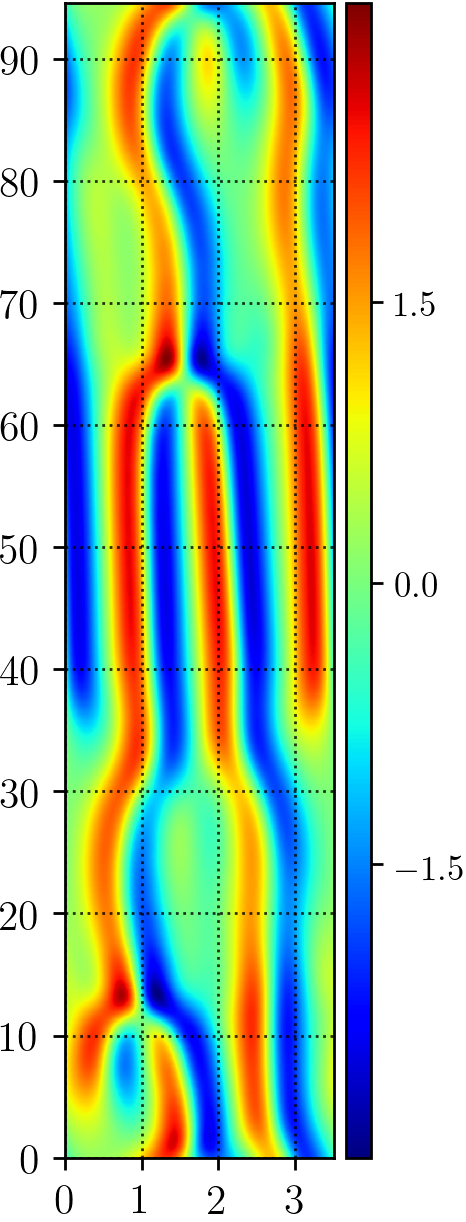
\includegraphics[width=.5\textwidth,height=.5\textheight]{MNG_halfdefect_defect_initial}
\end{minipage}
\begin{minipage}[height=.4\textheight]{.5\textwidth}
\centering \small{\texttt{(b)}}\\
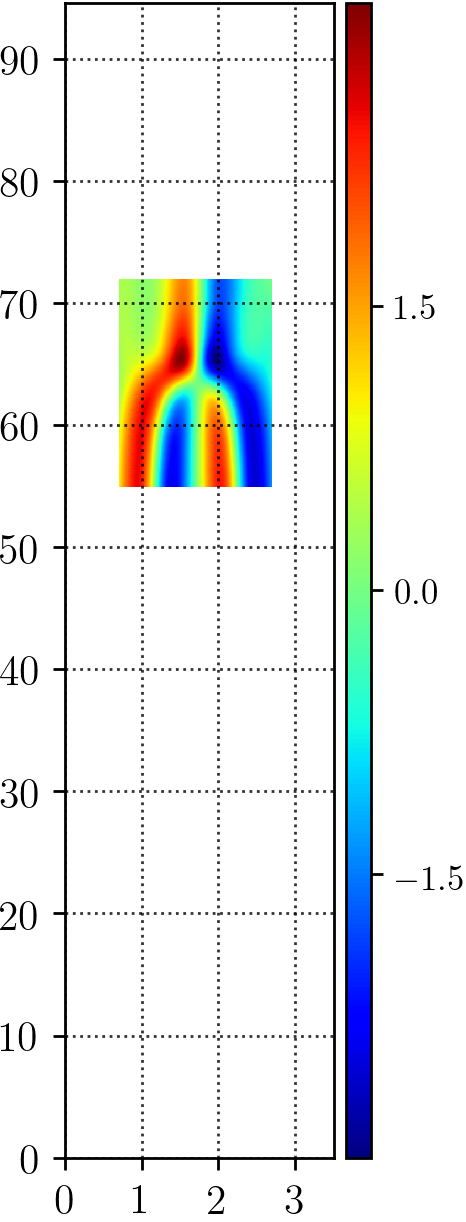
\includegraphics[width=.5\textwidth,height=.5\textheight]{MNG_defect_guess}
\end{minipage}
\begin{minipage}[height=.1\textheight]{\textwidth}
\centering \small{\texttt{(c)}}\\
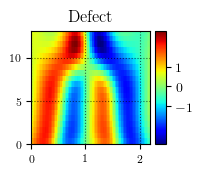
\includegraphics[width=.14\textwidth,height=.1\textheight]{MNG_defect}
\end{minipage}
\caption{ \label{fig:defect}
(a)
$[\speriod{a},\period{a}]=[3.50\cdots,94.59\cdots]$ fundamental domain
of an already computed \twot\ with spatial translation symmetry.
(b)
The clipped-out $[\speriod{b},\period{b}]=[2,17]$ subdomain used the
initial guess for the fundamental domain of a shift-reflect symmetric tile.
(c)
The converged $[\speriod{c},2\period{c}]=[2.07\cdots,18.46\cdots]$ \twot\
with spatial translation symmetry.
}
\end{figure}

\begin{figure}
\begin{minipage}[height=.4\textheight]{.5\textwidth}
\centering \small{\texttt{(a)}}\\
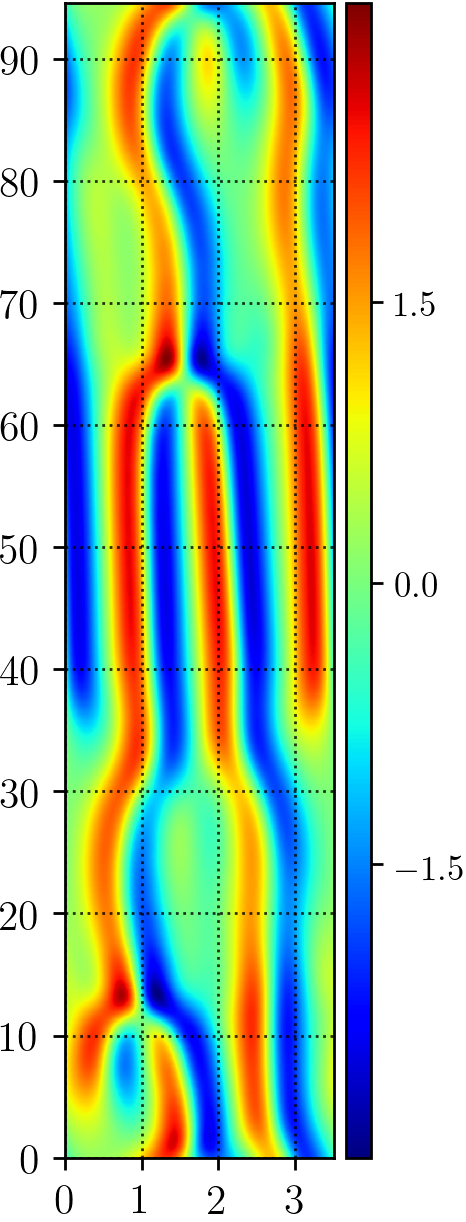
\includegraphics[width=.5\textwidth,height=.5\textheight]{MNG_halfdefect_defect_initial}
\end{minipage}
\begin{minipage}[height=.4\textheight]{.5\textwidth}
\centering \small{\texttt{(b)}}\\
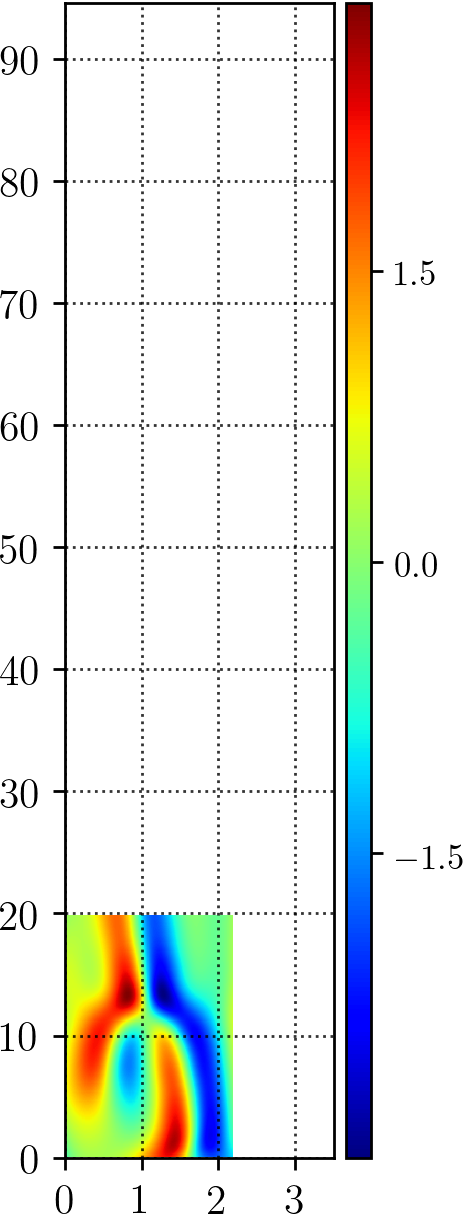
\includegraphics[width=.5\textwidth,height=.5\textheight]{MNG_halfdefect_guess}
\end{minipage}
\begin{minipage}[height=.1\textheight]{\textwidth}
\centering \small{\texttt{(c)}}\\
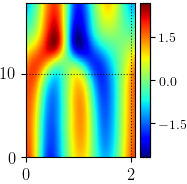
\includegraphics[width=.14\textwidth,height=.12\textheight]{MNG_halfdefect}
\end{minipage}
\caption{ \label{fig:halfdefect}
(a)
$[\speriod{a},\period{a}]=[3.50\cdots,94.59\cdots]$ fundamental domain
of an already computed \twot\ with spatial translation symmetry.
(b)
The clipped-out $[\speriod{b},\period{b}]=[2.2,20]$ subdomain used the
initial guess for the fundamental domain of a shift-reflect symmetric tile.
(c)
The converged $[\speriod{c},2\period{c}]=[2.07\cdots,15.46\cdots]$ \twot\
with spatial translation symmetry.
}
\end{figure}

\begin{figure}
\begin{minipage}[height=.4\textheight]{.5\textwidth}
\centering \small{\texttt{(a)}}\\
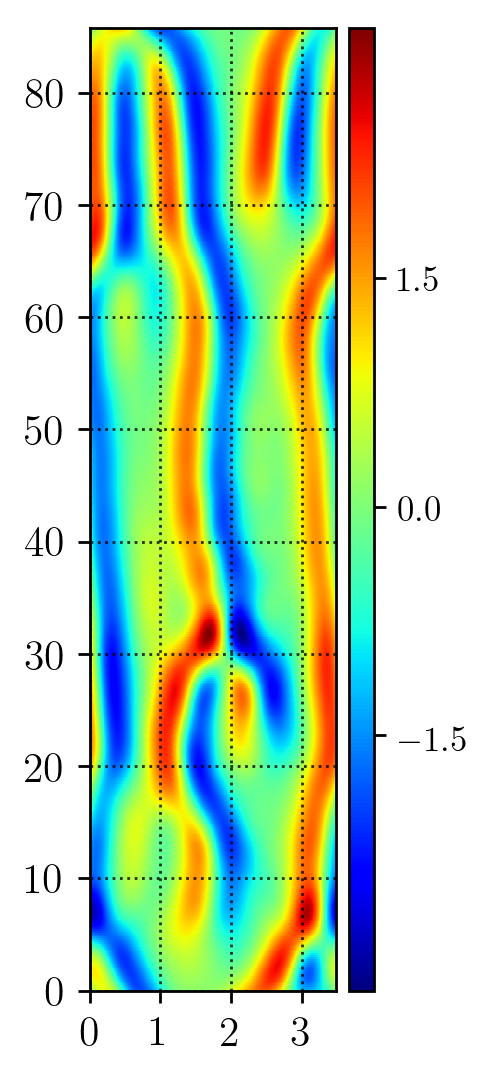
\includegraphics[width=.5\textwidth,height=.5\textheight]{MNG_halfdefect2_initial}
\end{minipage}
\begin{minipage}[height=.4\textheight]{.5\textwidth}
\centering \small{\texttt{(b)}}\\
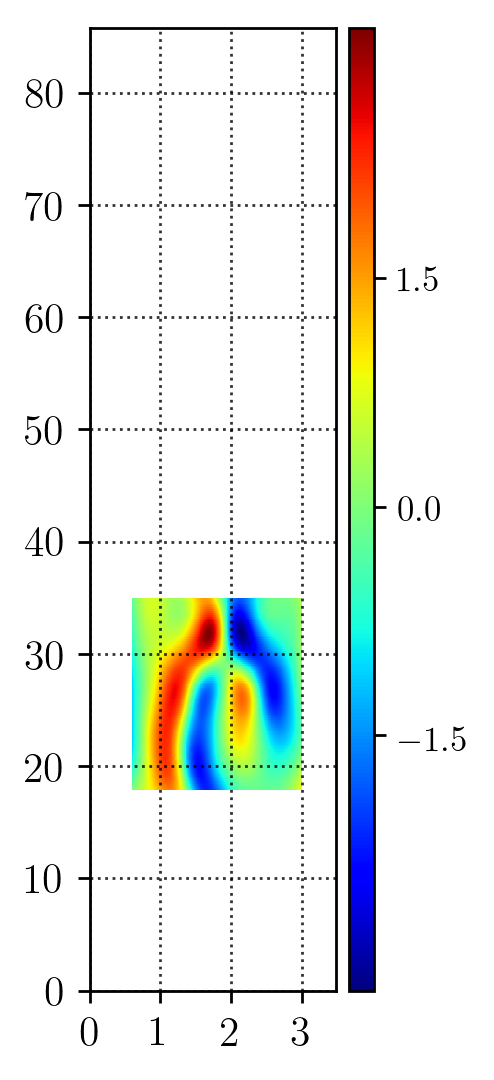
\includegraphics[width=.5\textwidth,height=.5\textheight]{MNG_halfdefect2_guess}
\end{minipage}
\begin{minipage}[height=.1\textheight]{\textwidth}
\centering \small{\texttt{(c)}}\\
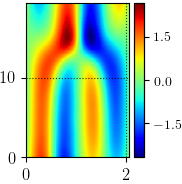
\includegraphics[width=.14\textwidth,height=.1\textheight]{MNG_halfdefect2}
\end{minipage}
\caption{ \label{fig:halfdefect2}
(a)
$[\speriod{a},\period{a}]=[3.50\cdots,85.73\cdots]$ fundamental domain
of an already computed \twot\ with \spt\ shift-reflection symmetry.
(b)
The clipped-out $[\speriod{b},\period{b}]=[2.6,17]$ subdomain used the
initial guess for the fundamental domain of a shift-reflect symmetric tile.
(c)
The converged $[\speriod{c},\period{c}]=[2.06\cdots,19.92\cdots]$ \twot\
with spatial translation symmetry.
}
\end{figure}

\begin{figure}
\begin{minipage}[height=.1\textheight]{.5\textwidth}
\centering \small{\texttt{(a)}}\\
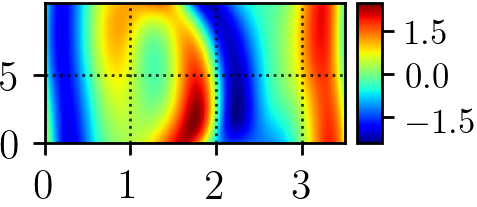
\includegraphics[width=.5\textwidth,height=.1\textheight]{MNG_hook_initial}
\end{minipage}
\begin{minipage}[height=.1\textheight]{.5\textwidth}
\centering \small{\texttt{(b)}}\\
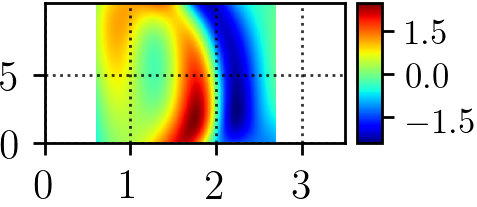
\includegraphics[width=.5\textwidth,height=.1\textheight]{MNG_hook_guess}
\end{minipage}
\begin{minipage}[height=.1\textheight]{\textwidth}
\centering \small{\texttt{(c)}}\\
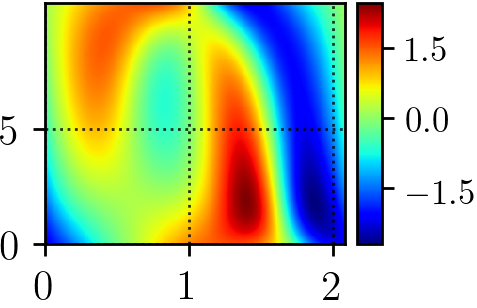
\includegraphics[width=.16\textwidth,height=.1\textheight]{MNG_hook}
\end{minipage}
\caption{ \label{fig:hook}
(a)
$[\speriod{a},\period{a}]=[3.50\cdots,10.25\cdots]$ fundamental domain
of an already computed \twot\ with \spt\ shift-reflection symmetry.
(b)
The clipped-out $[\speriod{b},\period{b}]=[2.1,10.5]$ subdomain used the
initial guess for the fundamental domain of a shift-reflect symmetric tile.
(c)
The converged $[\speriod{c},\period{c}]=[2.08\cdots,9.22\cdots]$  \twot\
with spatial translation symmetry.
}
\end{figure}

\begin{figure}
\begin{minipage}[height=.3\textheight]{.5\textwidth}
\centering \small{\texttt{(a)}}\\
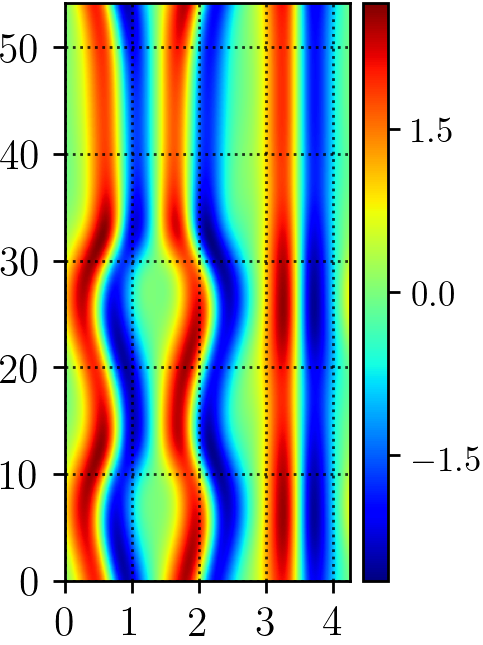
\includegraphics[width=.6\textwidth,height=.4\textheight]{MNG_gap_initial}
\end{minipage}
\begin{minipage}[height=.3\textheight]{.5\textwidth}
\centering \small{\texttt{(b)}}\\
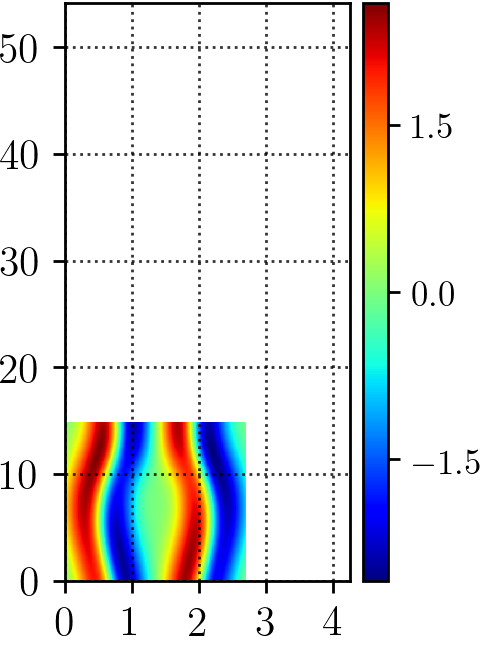
\includegraphics[width=.6\textwidth,height=.4\textheight]{MNG_gap_guess}
\end{minipage}
\begin{minipage}[height=.1\textheight]{\textwidth}
\centering \small{\texttt{(c)}}\\
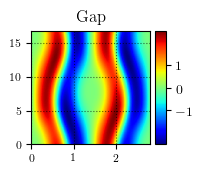
\includegraphics[width=.12\textwidth,height=.13\textheight]{MNG_gap}
\end{minipage}
\caption{ \label{fig:gap}
(a)
$[\speriod{a},\period{a}]=[4.25\cdots,54.13\cdots]$ fundamental domain
of an already computed \twot\ with \spt\ shift-reflection symmetry.
(b)
The clipped-out $[\speriod{b},\period{b}]=[2.7,15]$ subdomain used the
initial guess for the fundamental domain of a shift-reflect symmetric tile.
(c)
The converged $[\speriod{c},\period{c}]=[2.90\cdots,17.95\cdots]$ full
reflection symmetric \twot.
}
\end{figure}

\begin{figure}
\begin{minipage}[height=.2\textheight]{.5\textwidth}
\centering \small{\texttt{(a)}}\\
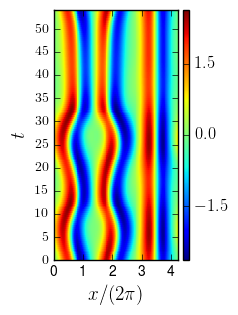
\includegraphics[width=.8\textwidth,height=.5\textheight]{MNGgapzero}
\end{minipage}
\begin{minipage}[height=.2\textheight]{.5\textwidth}
\centering \small{\texttt{(b)}}\\
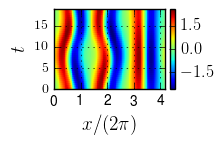
\includegraphics[width=.8\textwidth,height=.18\textheight]{MNGgapone}
\end{minipage}
\begin{minipage}[height=.2\textheight]{.5\textwidth}
\centering \small{\texttt{(c)}}\\
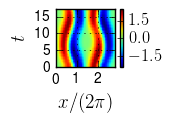
\includegraphics[width=.6\textwidth,height=.18\textheight]{MNGgaptwo}
\end{minipage}
\begin{minipage}[height=.2\textheight]{.48\textwidth}
\centering \small{\texttt{(d)}}\\
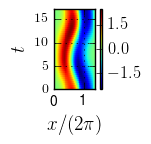
\includegraphics[width=.5\textwidth,height=.18\textheight]{MNGgapthree}
\end{minipage}
\caption{ \label{fig:KStileextraction}
Sequential subdomain extraction to find tiles.
(a) A {\po} from the collection of new solutions
$[\speriod{a},\period{a}]=[4.25\cdots,54.12\cdots]$.
By taking progressively smaller subdomains (b)-(d) and numerically
converging them to \twots\ at each step, we are able to
find the smallest subdomain of (a) which can be converges
to a \twot, namely (d).
(b)$[\speriod{b},\period{b}]=[4.16\cdots,18.93\cdots]$
(c)$[\speriod{c},\period{c}]=[2.79\cdots,17.14\cdots]$
(d)$[\speriod{d},\period{d}]=[1.39\cdots,17.14\cdots]$
}
\end{figure}

%Gluing
It should be noted that previously we claimed that
there are only three tiles. This is actually disingenuous because when we use tiles
in gluing access to their group orbit is used; that is, any symmetry copy or member
of their continuous family can be used. It is the tile's neighbors which
determines which family member is used in the gluing process.
There are many uses for the process of gluing; the most important being the
eventually explanation of infinite space-time by virtue of \spt\ symbolic
dynamics

\begin{figure}
\centering
\begin{minipage}[height=.4\textheight]{.66\textwidth}
\centering
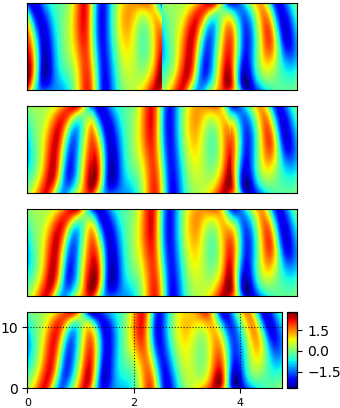
\includegraphics[width=.7\textwidth,height=.6\textheight]{MNGppo12space_glue}
\end{minipage}
\caption{ \label{fig:MNGppo12spaceglue}
Spatial gluing of the two shortest shift-reflection
\twots. The sizes of the fundamental domains of these
\twots\ are
$[\speriod{1},\period{1}]=[3.5\cdots,20.50\cdots]$
and
$[\speriod{2},\period{2}]=[3.5\cdots,28.66\cdots]$
respectively.
The result is a
shift-reflection \twot\ with
$[\speriod{1,2},\period{1,2}]=[6.79\cdots,24.82\cdots]$
fundamental domain.
}
\end{figure}


\begin{figure}
\begin{minipage}[height=.4\textheight]{.99\textwidth}
\centering
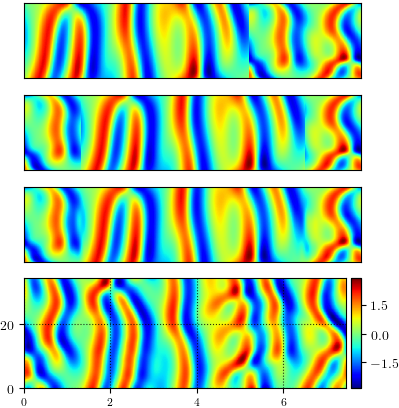
\includegraphics[width=.99\textwidth,height=.66\textheight]{MNGppo123space_glue}
\end{minipage}
\caption{ \label{fig:ppo123spaceglue}
Gluing procedure which spatially combines the third shortest (period) shift-reflection
invariant
$[\speriod{3},\period{3}]=[3.5\cdots,64.70\cdots]$
\twot\
 with the resultant shift-reflection invariant \twot\
from
\PCedit{reffig{fig:ppo12spaceglue}} %2019-12-06
with
$[\speriod{1,2},\period{1,2}]=[6.79\cdots,24.82\cdots]$
fundamental domain.
This results in another shift-reflection
\twot\ with the
$[\speriod{1,2,3},\period{1,2,3}]=[10.53\cdots,68.84\cdots]$
 fundamental domain.
The dramatic change between the last
two panels is presumably an effect of the
discrepancy between the temporal period of
the constituent solutions.
}
\end{figure}


\begin{figure}
\centering
\begin{minipage}[height=.4\textheight]{.66\textwidth}
\centering
\includegraphics[width=.7\textwidth,height=.6\textheight]{MNG_ppolargeTspaceglue}
\end{minipage}
\caption{ \label{fig:MNGppo12spaceglue1}
Spatial gluing of the two shortest shift-reflection
\twots. The sizes of the fundamental domains of these
\twots\ are
$[\speriod{1},\period{1}]=[3.5\cdots,20.50\cdots]$
and
$[\speriod{2},\period{2}]=[3.5\cdots,28.66\cdots]$
respectively.
The result is a
shift-reflection \twot\ with
$[\speriod{1,2},\period{1,2}]=[6.79\cdots,24.82\cdots]$
fundamental domain.
}
\end{figure}


\begin{figure}
\centering
\begin{minipage}[height=.4\textheight]{.66\textwidth}
\centering
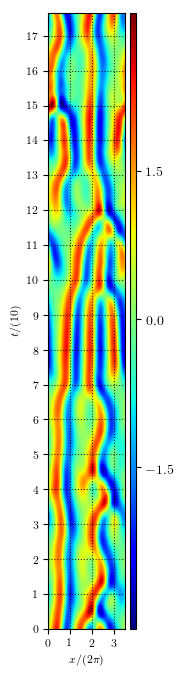
\includegraphics[width=.7\textwidth,height=.6\textheight]{MNG_rpoLargeTtimeglue}
\end{minipage}
\caption{ \label{fig:MNGppo12spaceglue2}
Spatial gluing of the two shortest shift-reflection
\twots. The sizes of the fundamental domains of these
\twots\ are
$[\speriod{1},\period{1}]=[3.5\cdots,20.50\cdots]$
and
$[\speriod{2},\period{2}]=[3.5\cdots,28.66\cdots]$
respectively.
The result is a
shift-reflection \twot\ with
$[\speriod{1,2},\period{1,2}]=[6.79\cdots,24.82\cdots]$
fundamental domain.
}
\end{figure}


\begin{figure}
\begin{minipage}[height=.4\textheight]{.5\textwidth}
\centering \small{\texttt{(a)}}\\
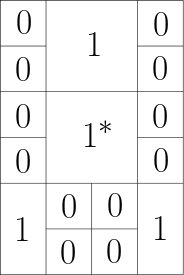
\includegraphics[width=.5\textwidth,height=.25\textheight]{MNG_symbolicblock}
\end{minipage}
\begin{minipage}[height=.4\textheight]{.5\textwidth}
\centering \small{\texttt{(b)}}\\
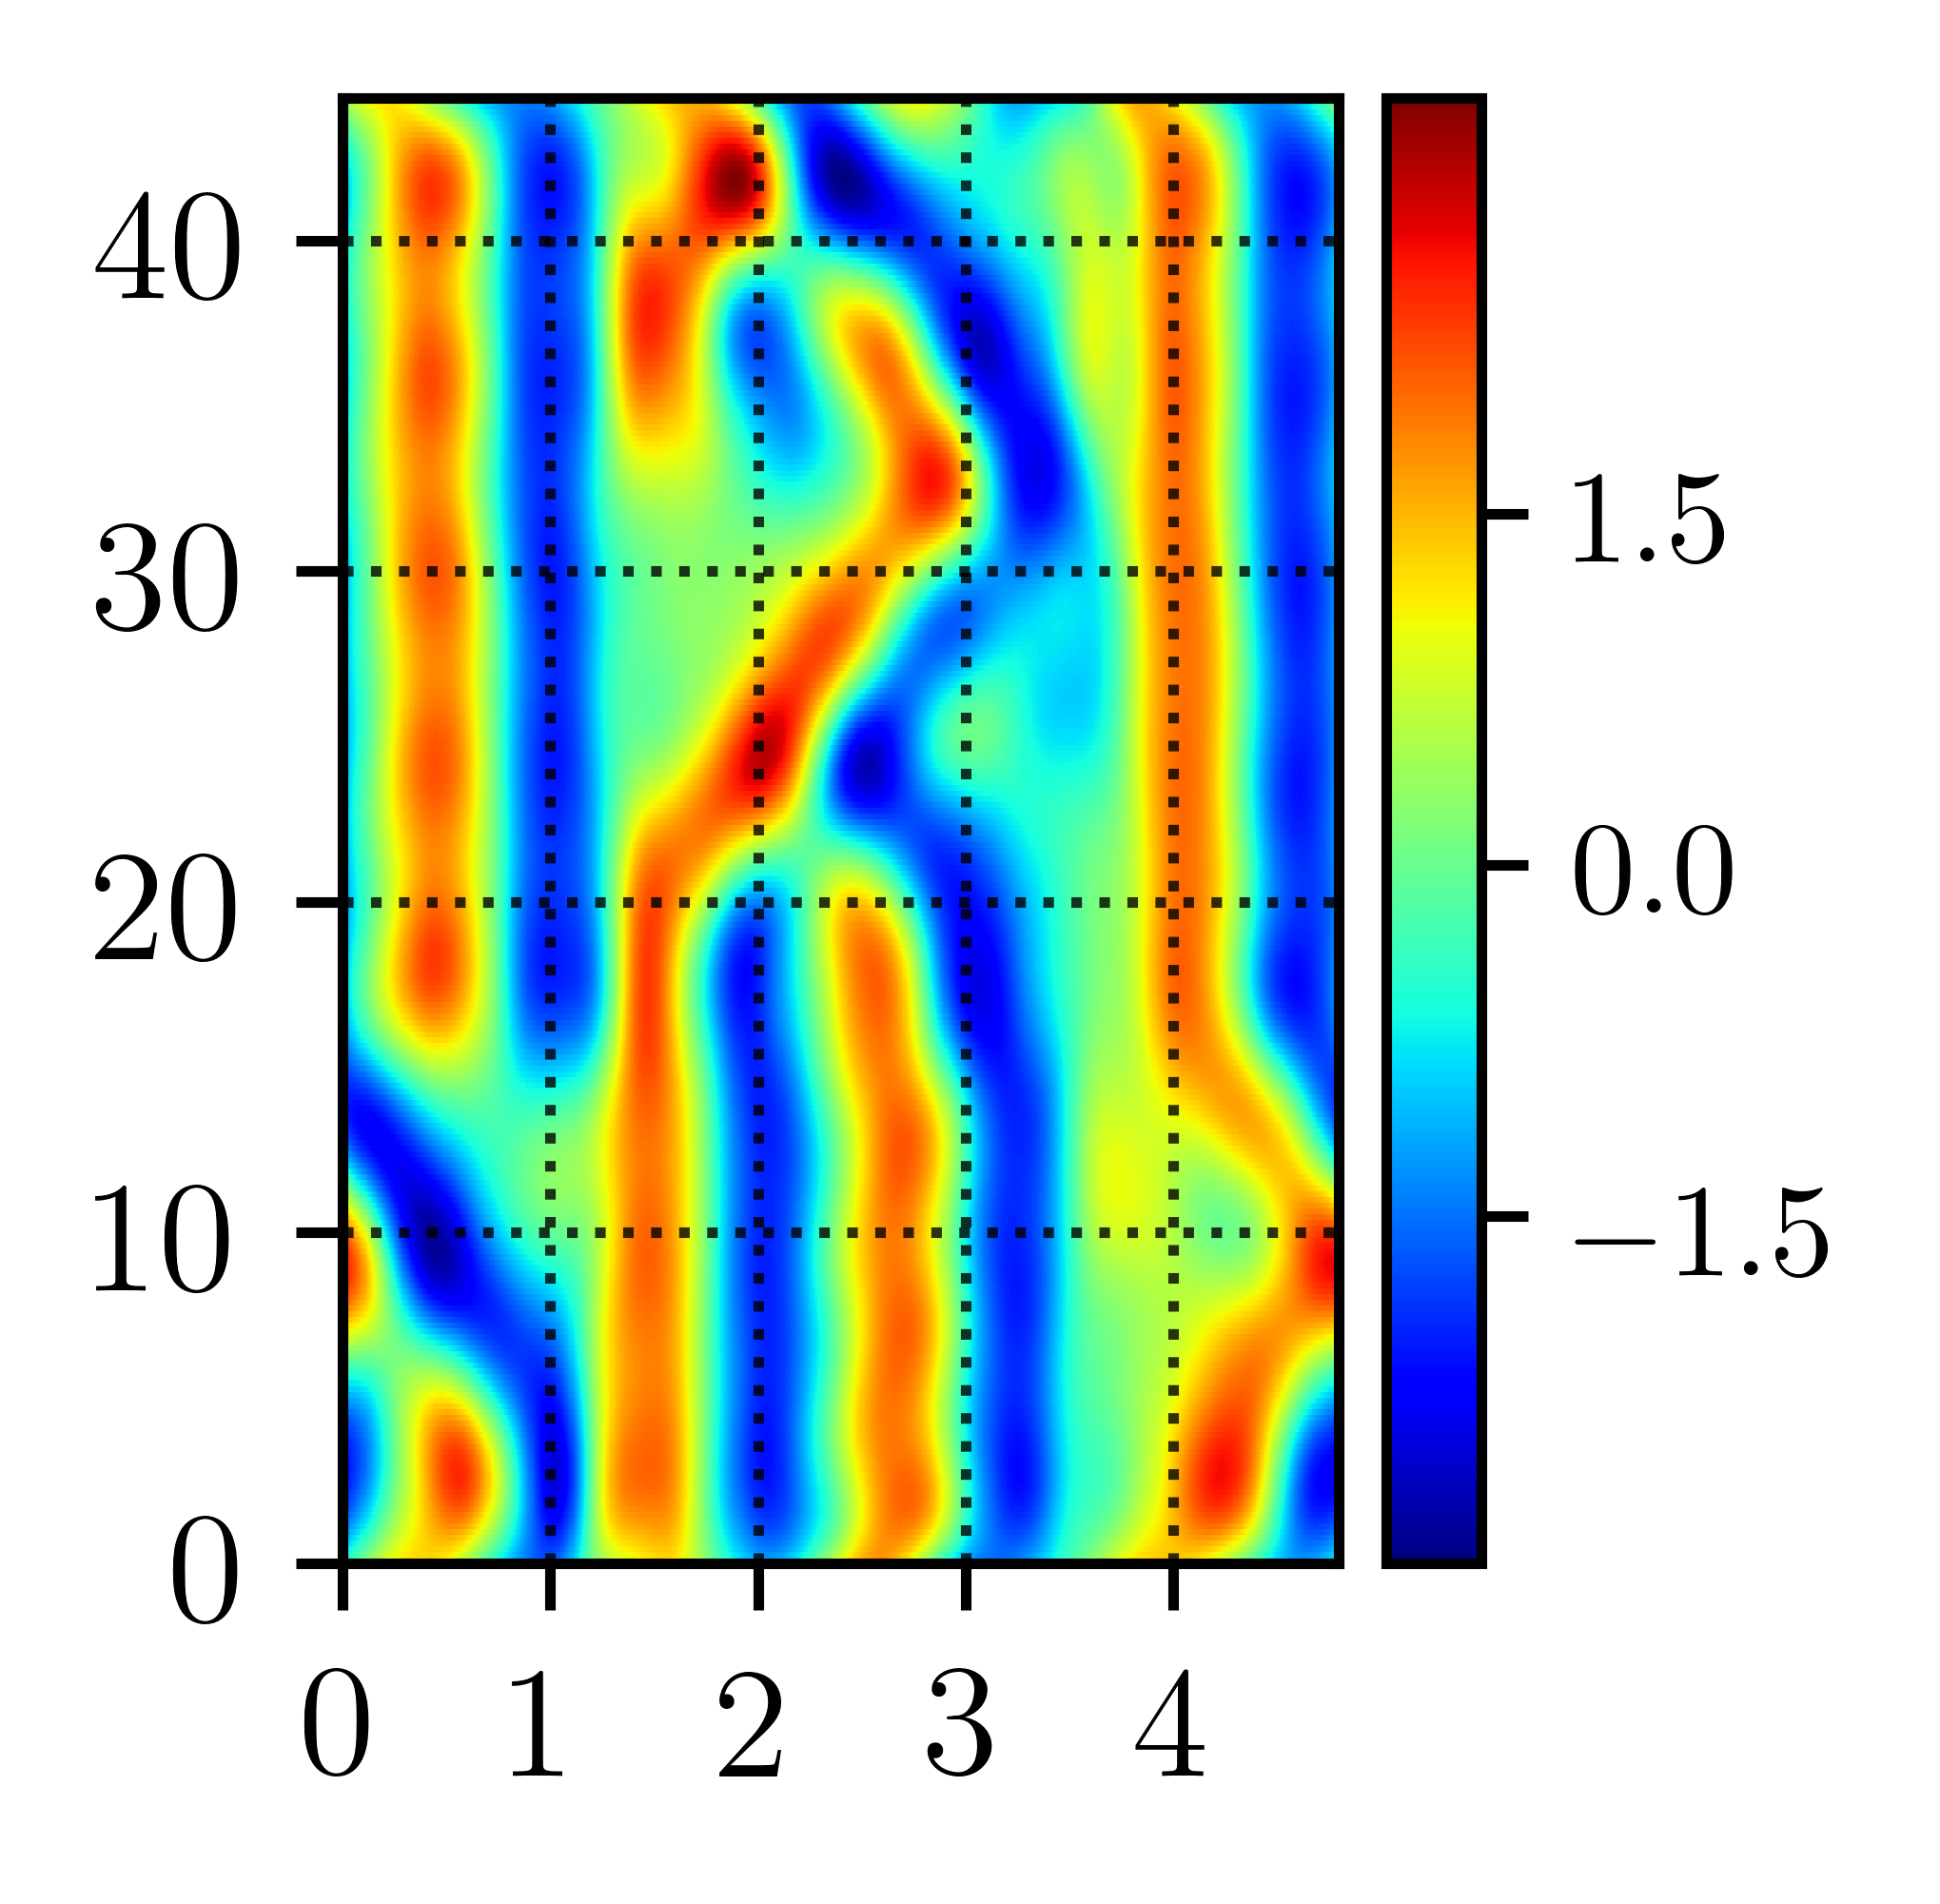
\includegraphics[width=.7\textwidth,height=.32\textheight]{MNG_trinary_initial}
\end{minipage}
\begin{minipage}[height=.4\textheight]{.5\textwidth}
\centering \small{\texttt{(c)}}\\
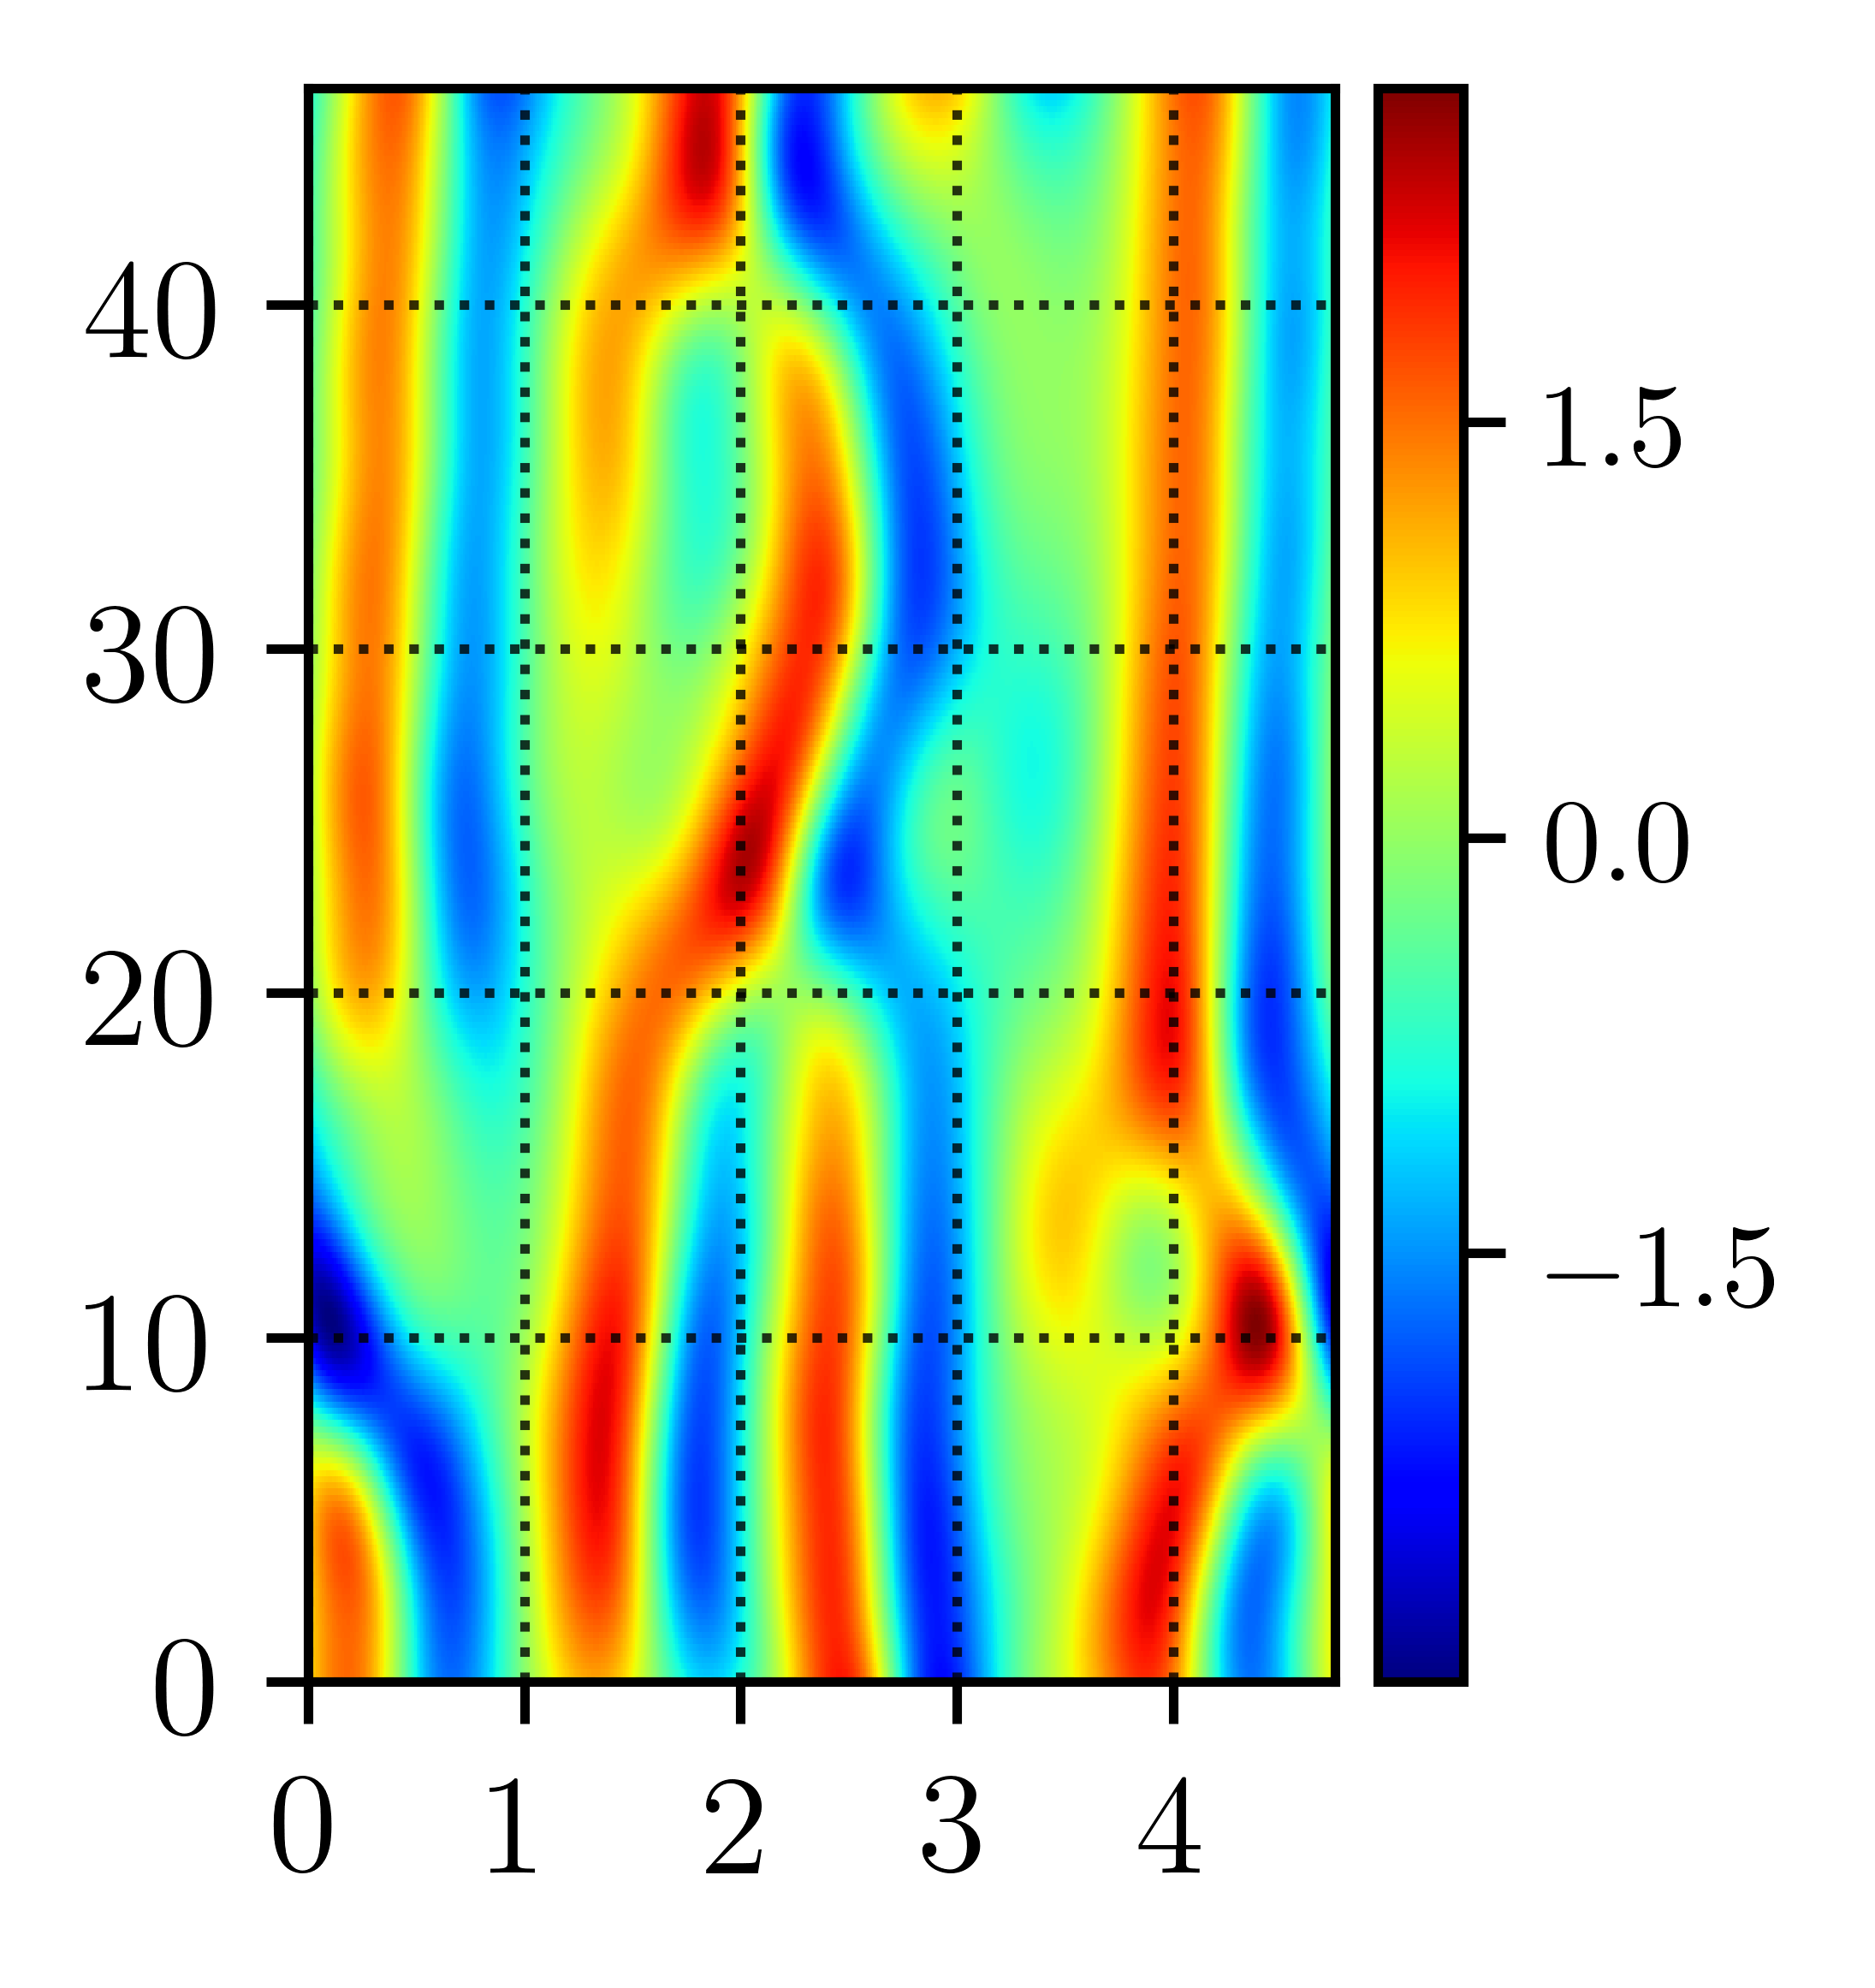
\includegraphics[width=.7\textwidth,height=.32\textheight]{MNG_trinary_final}
\end{minipage}
\begin{minipage}[height=.4\textheight]{.5\textwidth}
\centering \small{\texttt{(d)}}\\
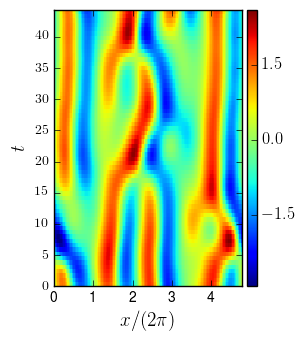
\includegraphics[width=.7\textwidth,height=.32\textheight]{MNG_ppo_L30_T44}
\end{minipage}
\caption{ \label{fig:trinarytiling}
(a) \Spt\ symbolic block representation created using group orbits
of three tile families,
(b) initial condition produced by combining tiles according to (a);
dimensions initialized at $[\speriod{b},\period{b}]=[4.79\cdots,88.62\cdots]$,
(c) converged \twot\ when using (b) as an initial condition,
(d) targeted \twot\ which (c) was trying to match.
}
\end{figure}


\begin{figure}
\begin{minipage}[height=.05\textheight]{.3\textwidth}
\centering \small{\texttt{(a)}}\\
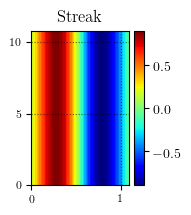
\includegraphics[width=.3\textwidth,height=.1\textheight]{MNG_streak}
\end{minipage}
\begin{minipage}[height=.05\textheight]{.3\textwidth}
\centering \small{\texttt{(b)}}\\
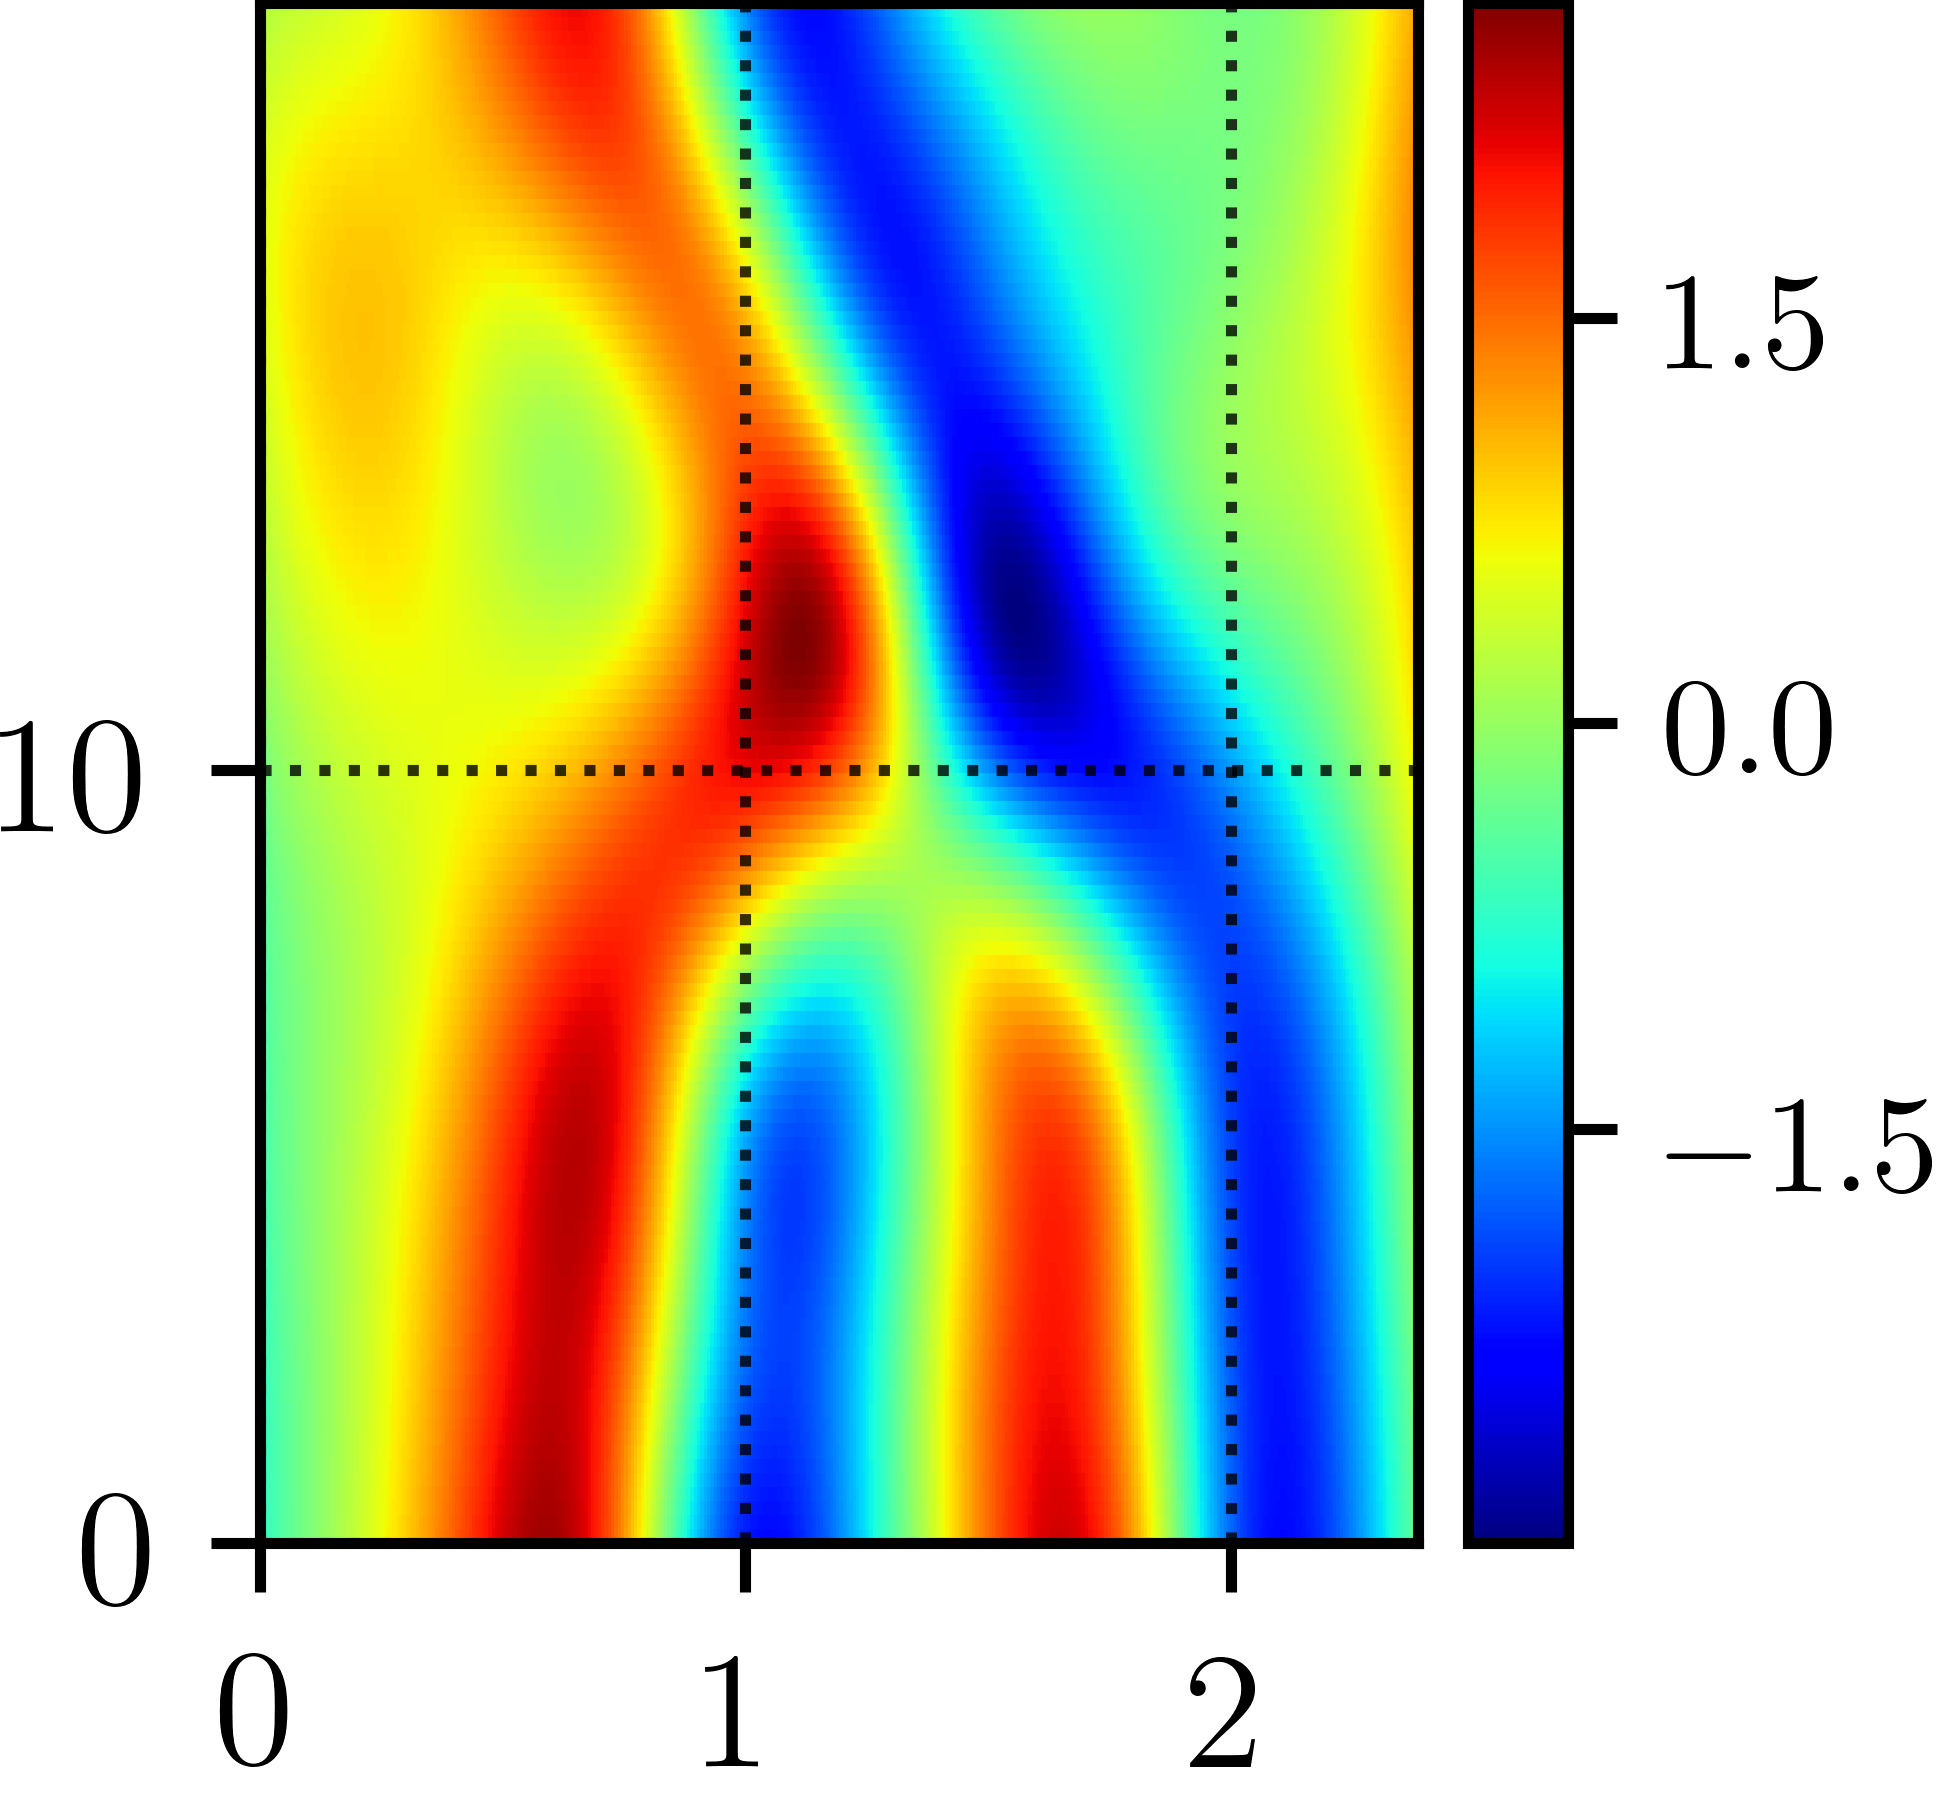
\includegraphics[width=.4\textwidth,height=.1\textheight]{MNG_hookondefecterg}
\end{minipage}
\begin{minipage}[height=.05\textheight]{.3\textwidth}
\centering \small{\texttt{(c)}}\\
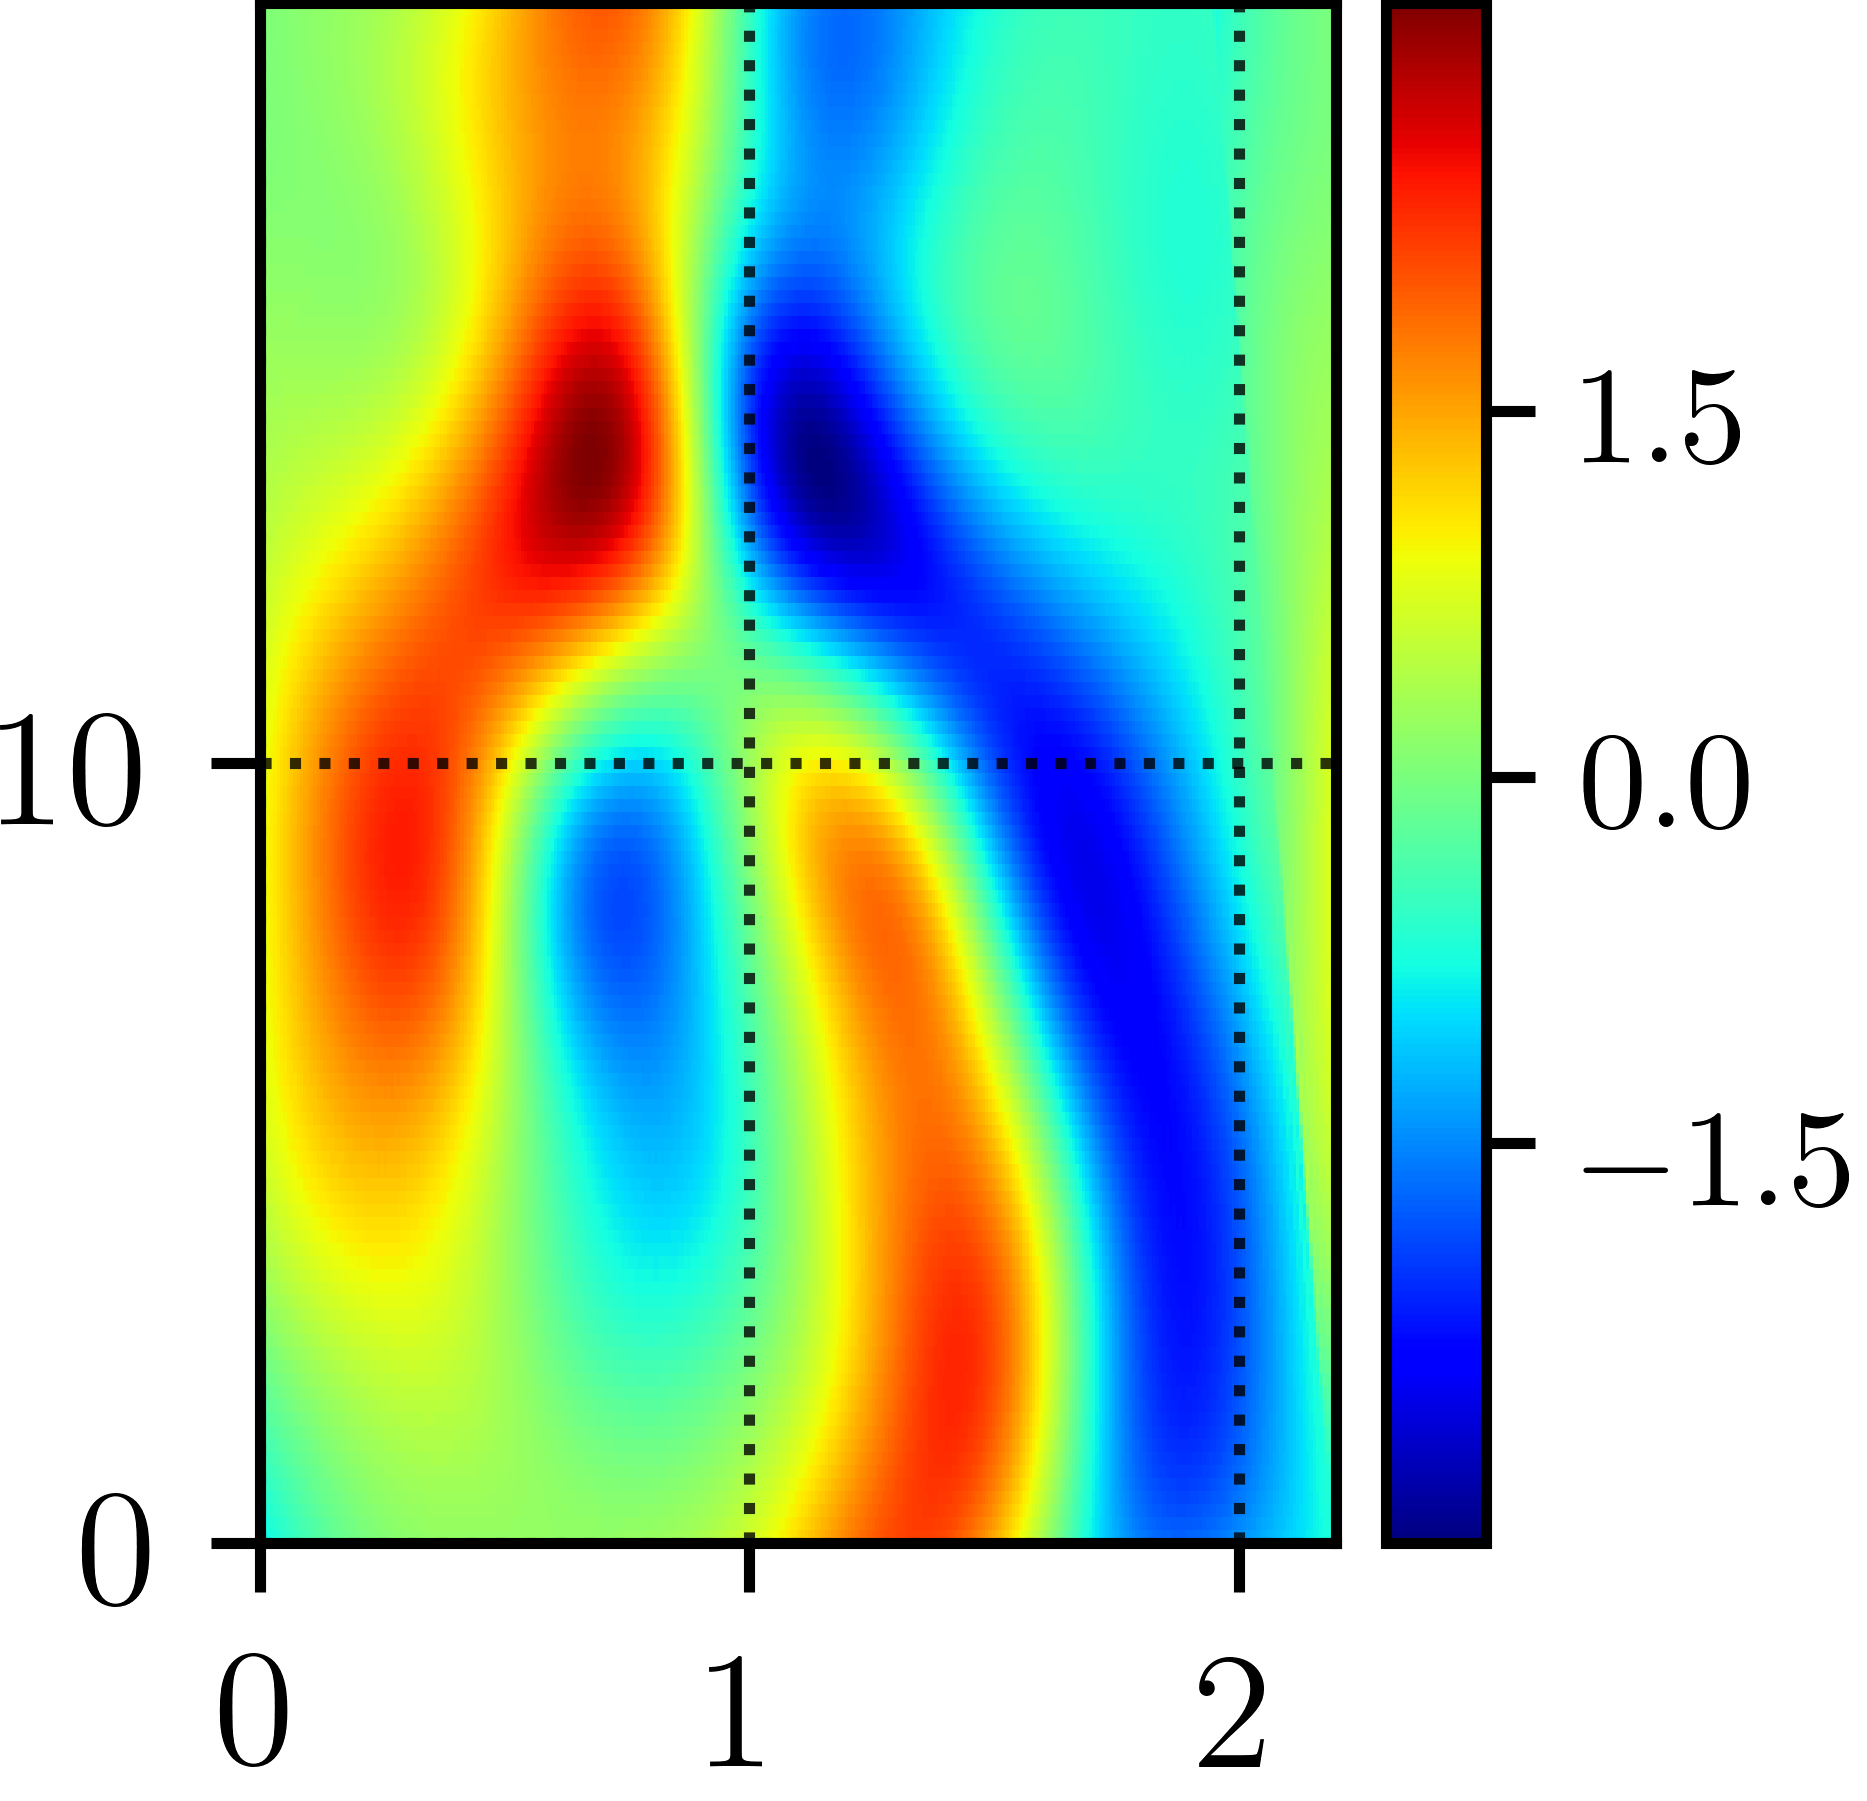
\includegraphics[width=.4\textwidth,height=.1\textheight]{MNG_halfdefecterg}
\end{minipage}
\begin{minipage}[height=.05\textheight]{.3\textwidth}
\centering \small{\texttt{(d)}}\\
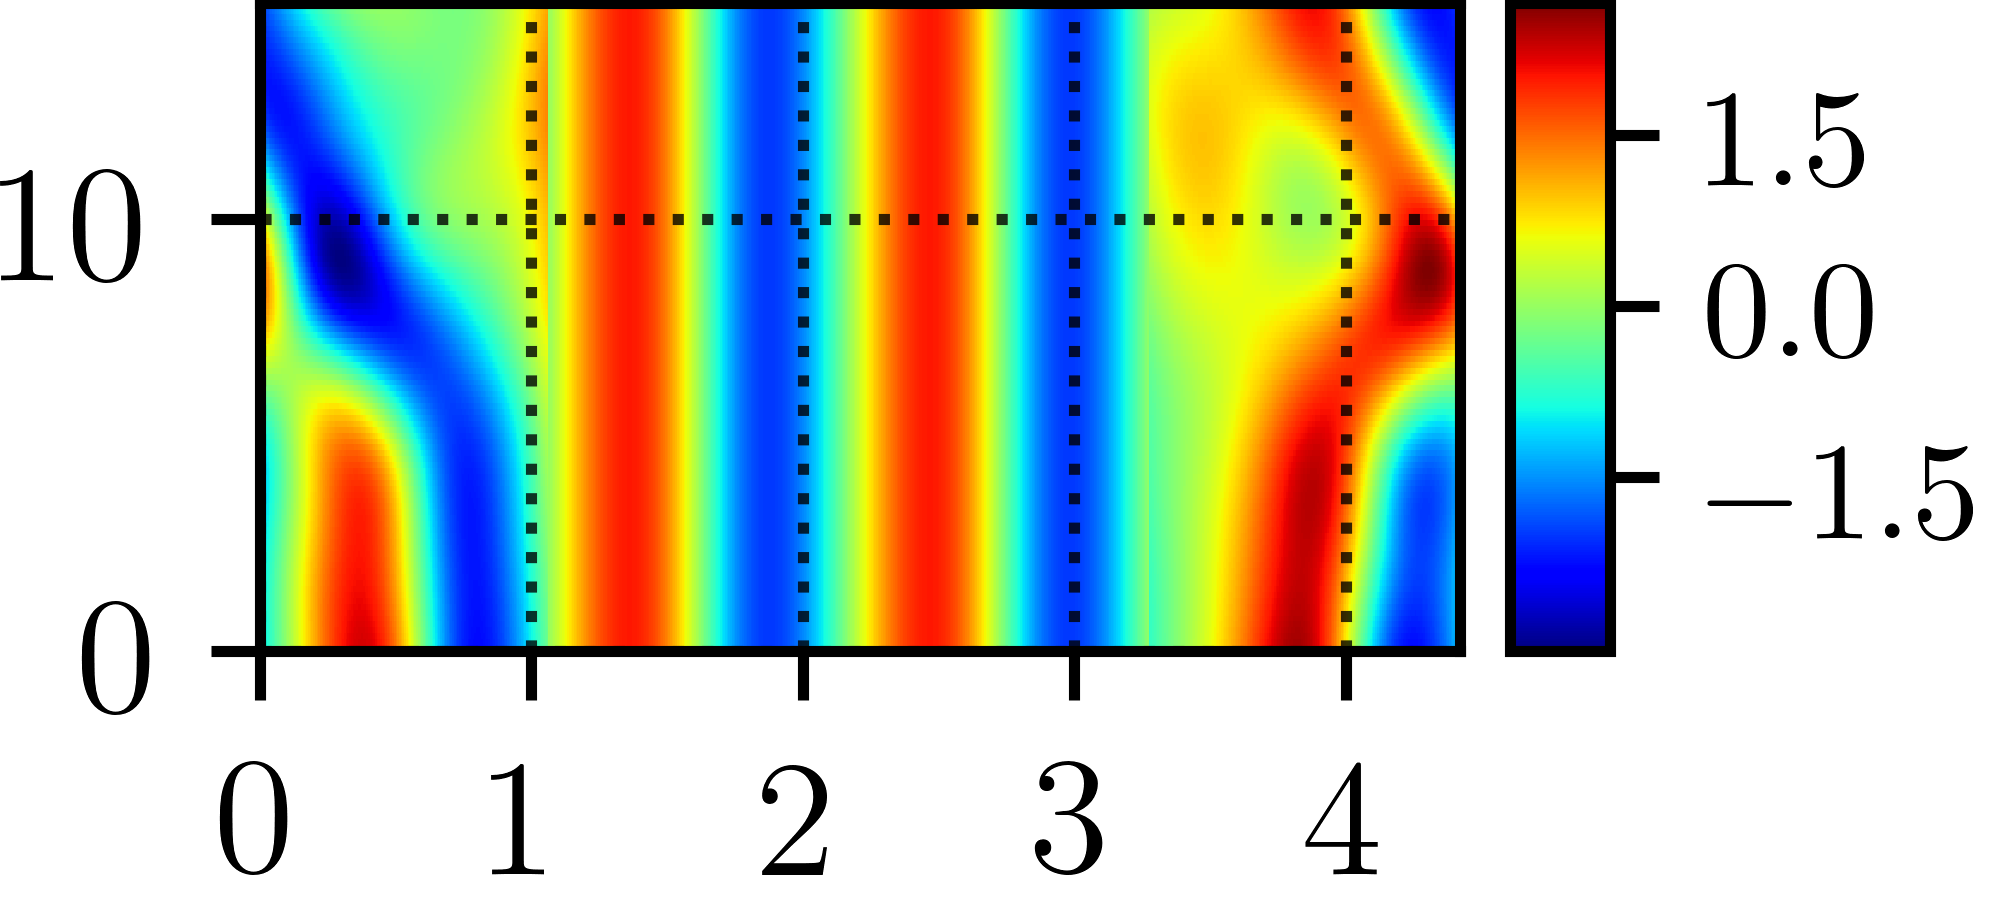
\includegraphics[width=.8\textwidth,height=.1\textheight]{MNG_tiling_subdomain0}
\end{minipage}
\begin{minipage}[height=.05\textheight]{.3\textwidth}
\centering \small{\texttt{(e)}}\\
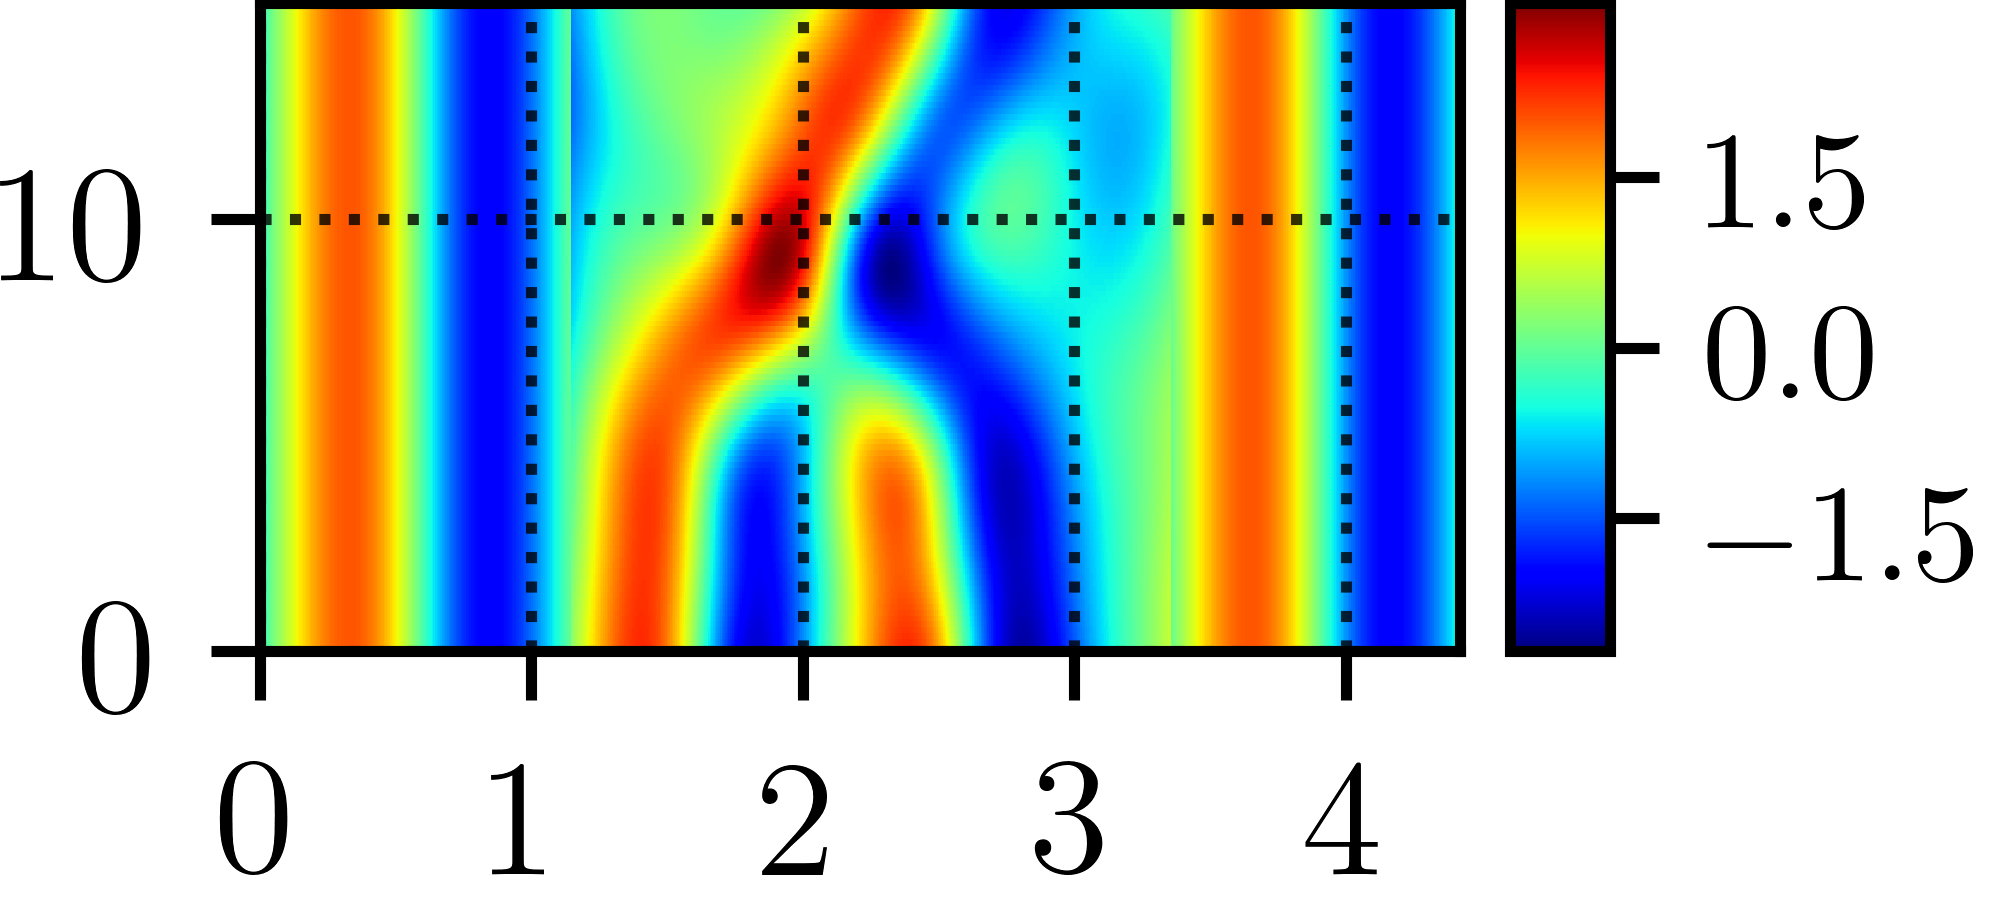
\includegraphics[width=.8\textwidth,height=.1\textheight]{MNG_tiling_subdomain1}
\end{minipage}
\begin{minipage}[height=.05\textheight]{.3\textwidth}
\centering \small{\texttt{(f)}}\\
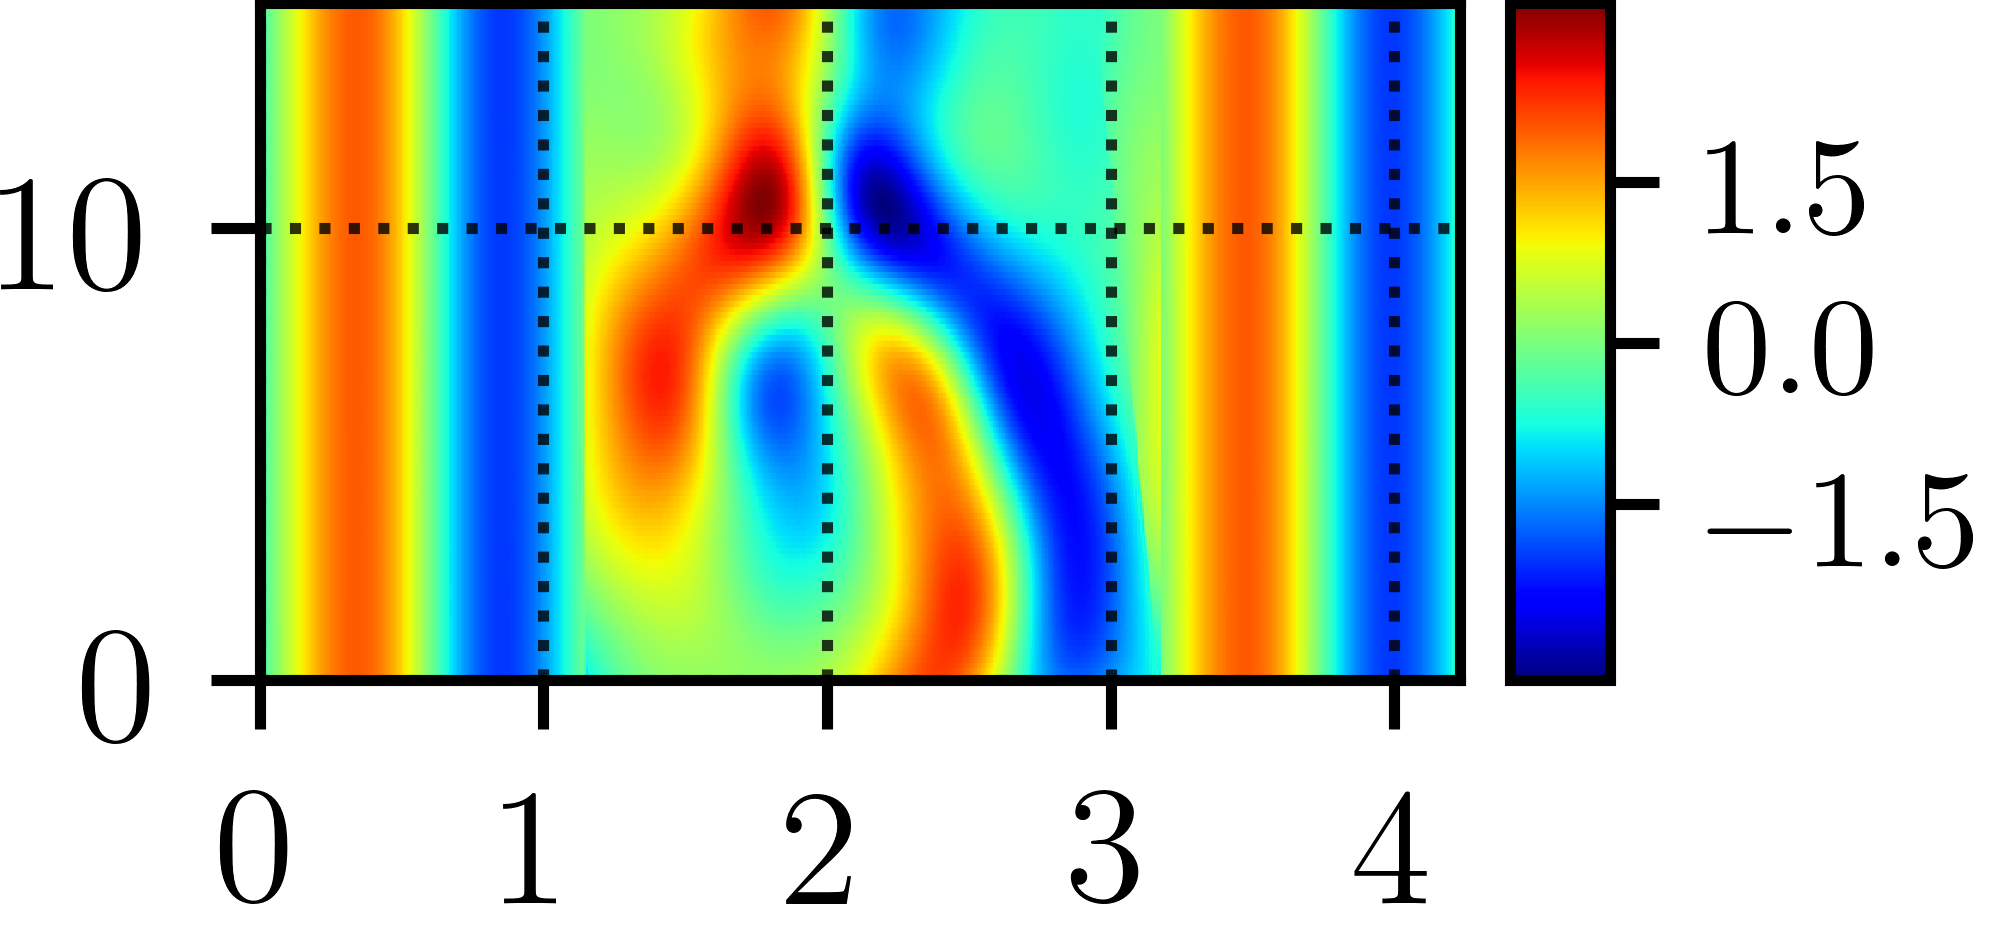
\includegraphics[width=.8\textwidth,height=.1\textheight]{MNG_tiling_subdomain2}
\end{minipage}
\begin{minipage}[height=.1\textheight]{.35\textwidth}
\centering \small{\texttt{(g)}}\\
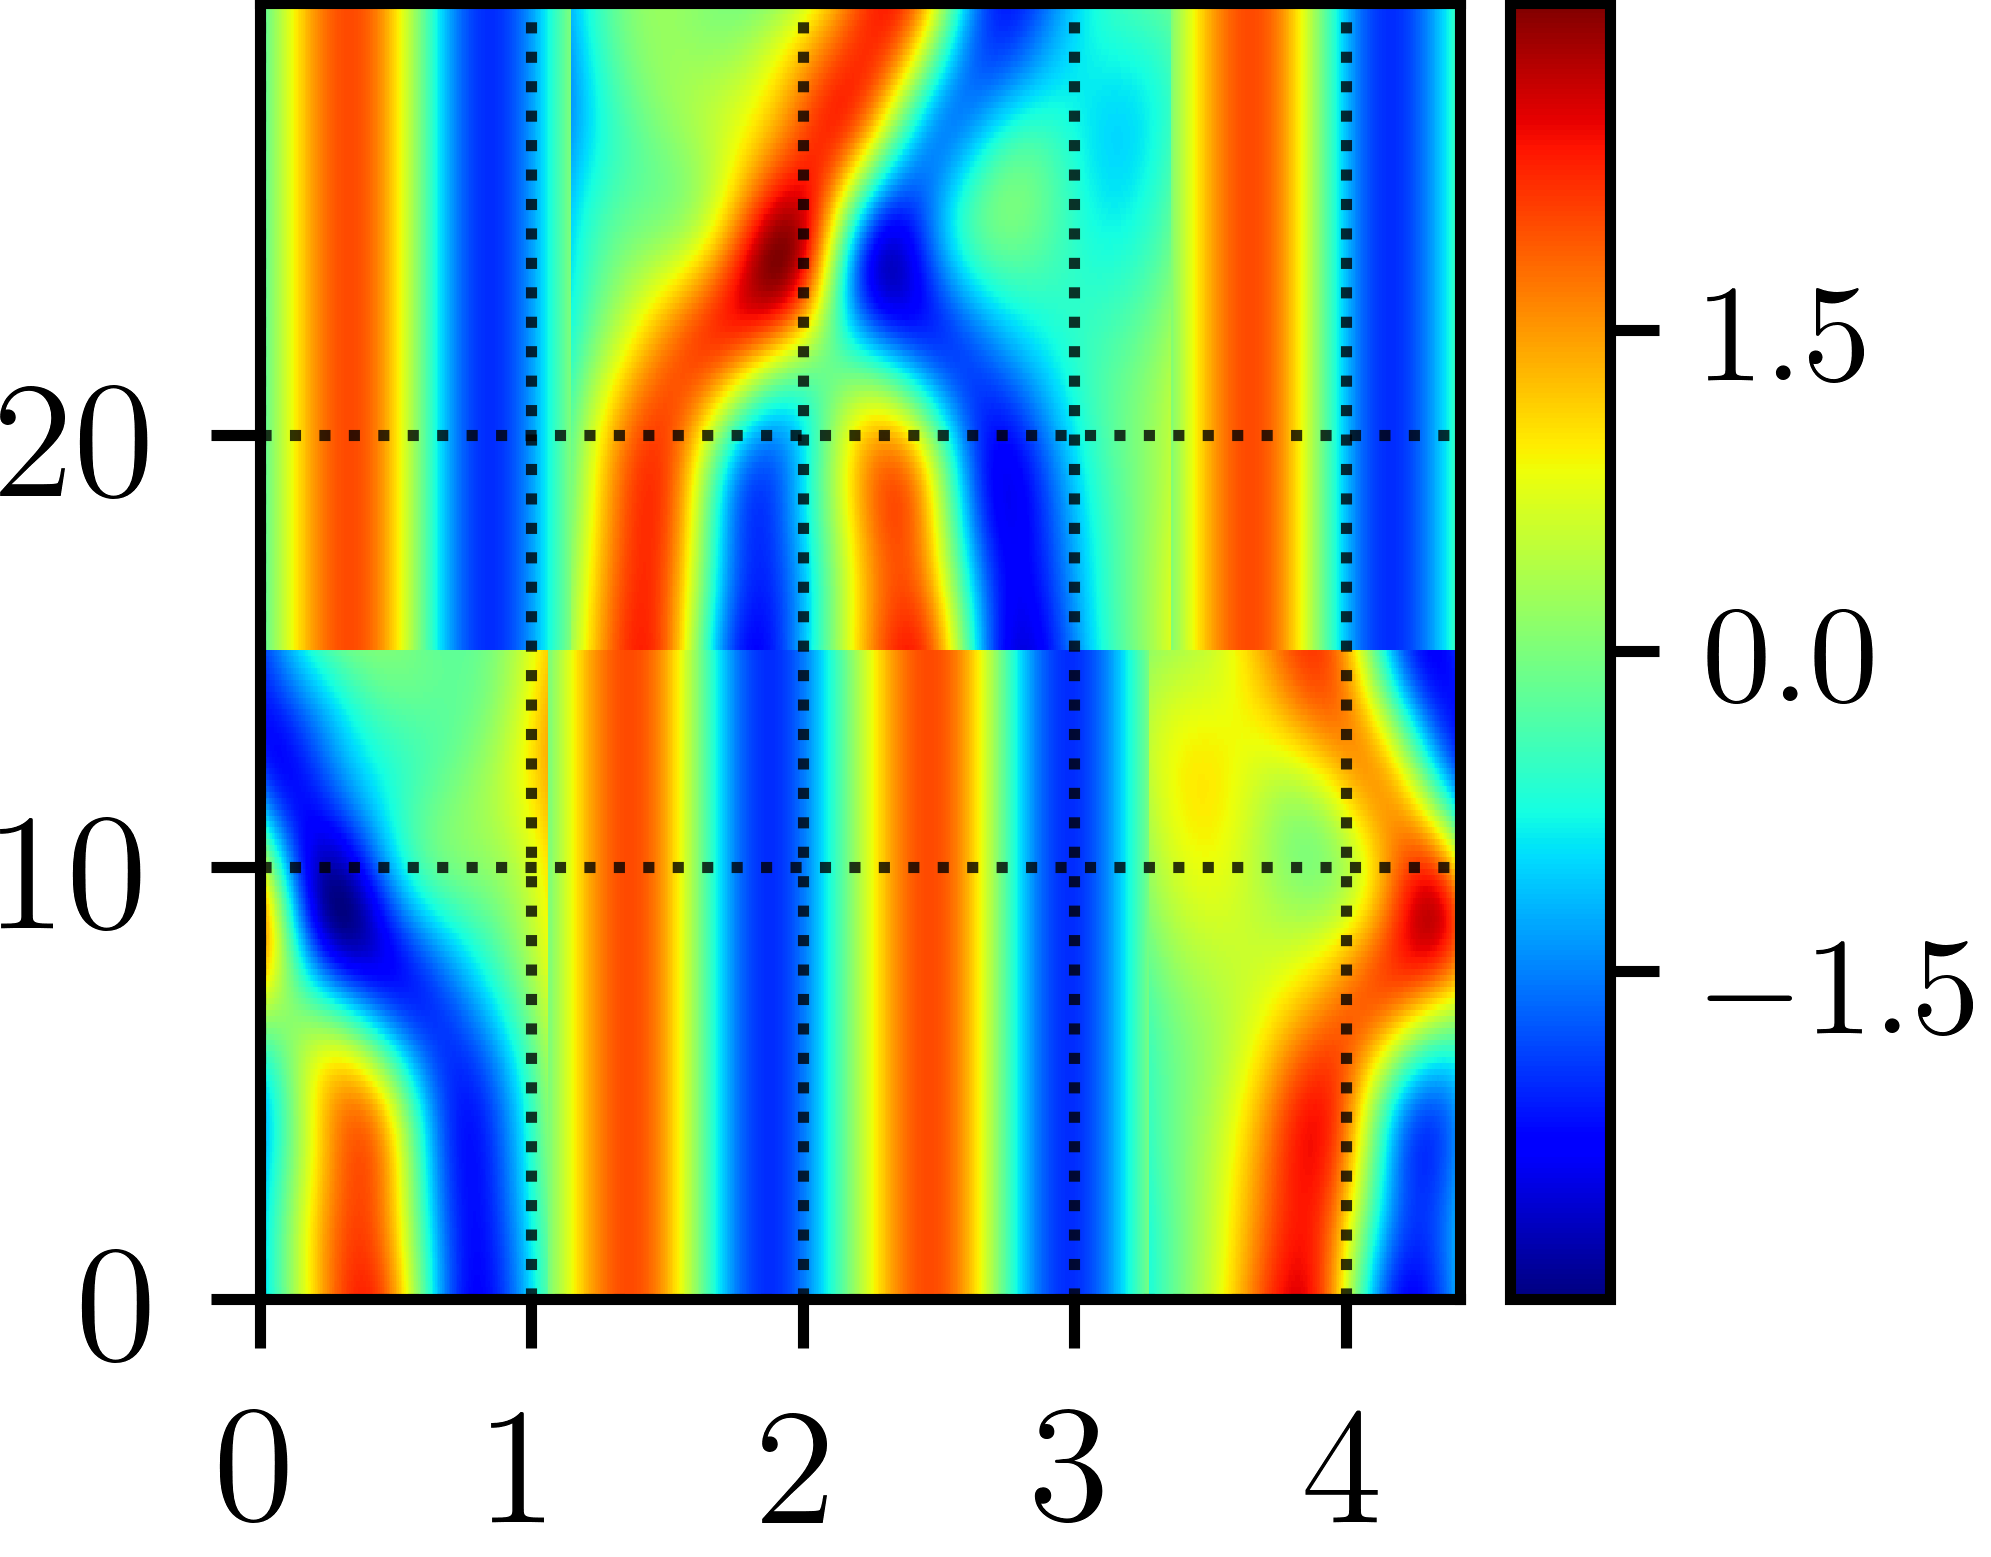
\includegraphics[width=.8\textwidth,height=.28\textheight]{MNG_tiling_twosubdomains}
\end{minipage}
\begin{minipage}[height=.15\textheight]{.3\textwidth}
\centering \small{\texttt{(h)}}\\
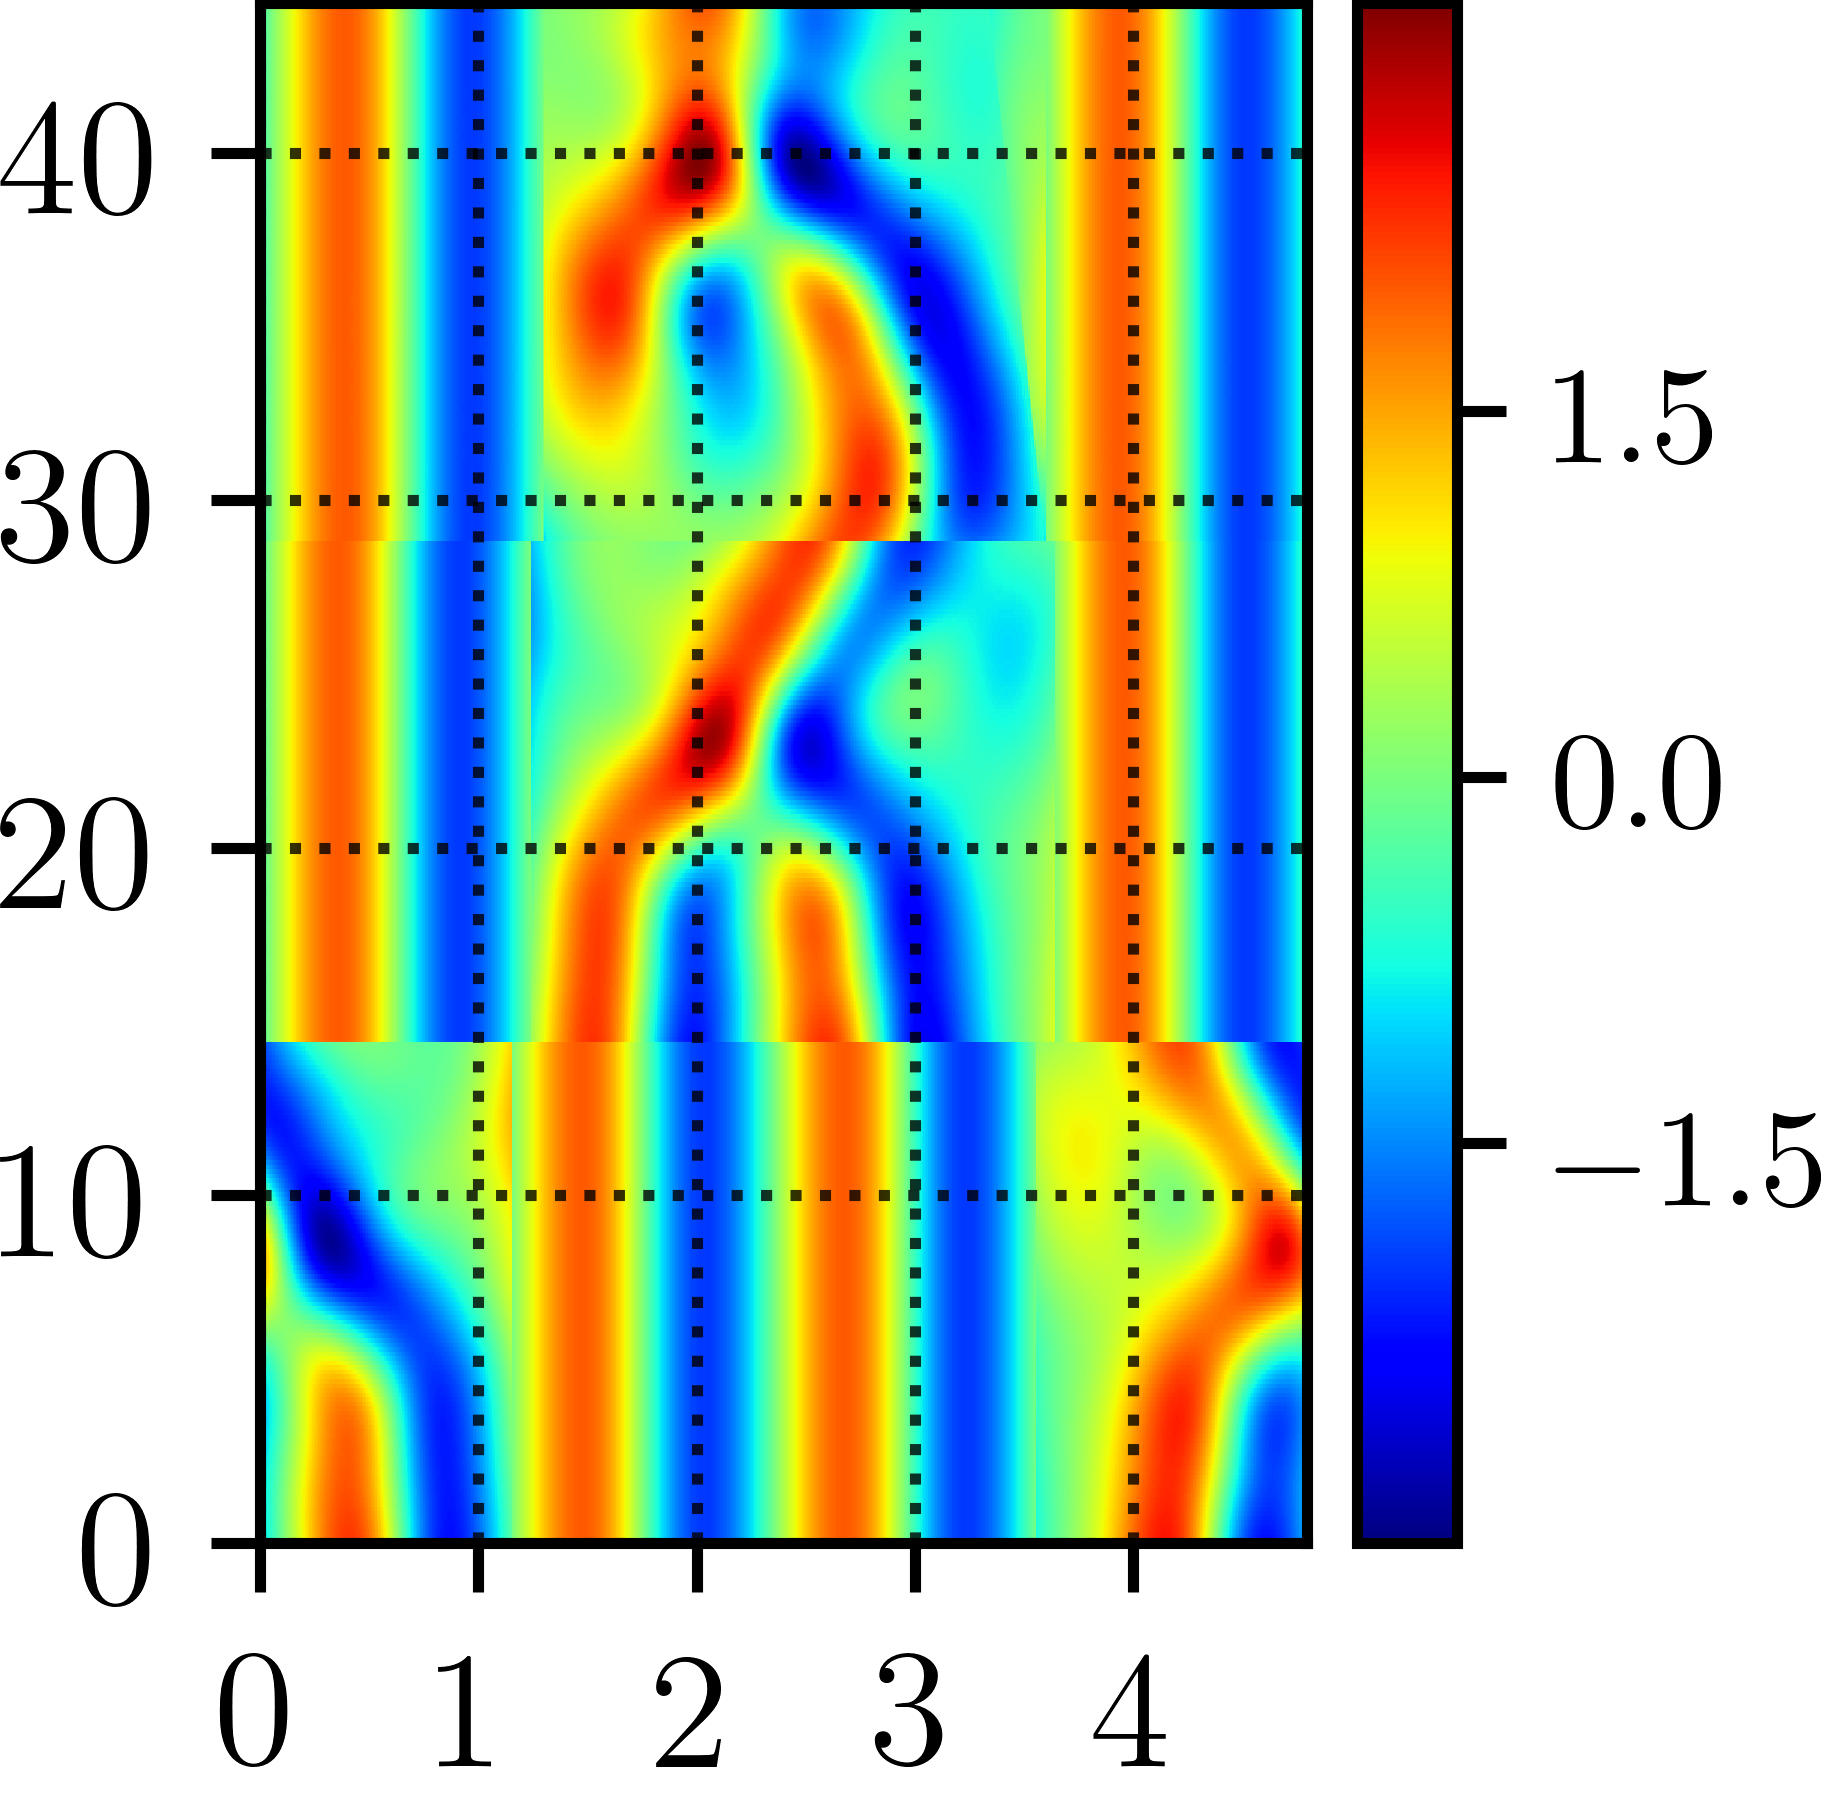
\includegraphics[width=\textwidth,height=.36\textheight]{MNG_tiling_fundamental}
\end{minipage}
\begin{minipage}[height=.15\textheight]{.3\textwidth}
\centering \small{\texttt{(i)}}\\
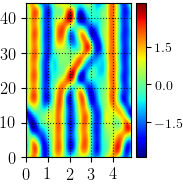
\includegraphics[width=\textwidth,height=.36\textheight]{MNG_tiling_initial}
\end{minipage}

\caption{ \label{fig:tilingschematic}
Demonstration of how to construct an initial condition corresponding to a specific
\spt\ symbolic block. (a),(b) and (c) together are the set of tiles used for all
other plots in this figure. (d) is a subdomain comprised of two copies of (a) and one copy of (b). (e) is a subdomain comprised of two copies of (a) and one copy of
the reflection of (b). (f) is a subdomain comprised of two copies of (a) and a
single copy of (c). The last row of figures demonstrate how to combine (d),(e),
and (f). (g) is the combination of (d) and (e). (h) is the combination of (d),(e)
and (f) (equivalently, (g) and (f)). Lastly (i) is the smoothed version of (h) which will serve as the initial condition.
}
\end{figure}


\begin{figure}
\begin{minipage}[height=.4\textheight]{.5\textwidth}
\centering \small{\texttt{(a)}}\\
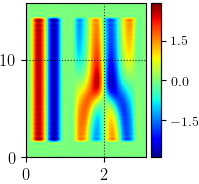
\includegraphics[width=.3\textwidth,height=.15\textheight]{MNG_01_initial}
\end{minipage}
\begin{minipage}[height=.4\textheight]{.5\textwidth}
\centering \small{\texttt{(b)}}\\
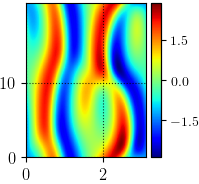
\includegraphics[width=.3\textwidth,height=.18\textheight]{MNG_01_final}
\end{minipage}
\caption{ \label{fig:block01}
(a) Initial \spt\ field for the one-by-two symbolic block given by \refeq{e-block01}
(b) \twoT\ resultant from numerically converging (a),
$[\speriod{b},\period{b}]=[3.13\cdots,20.84\cdots]$
}
\end{figure}

\begin{figure}
\begin{minipage}[height=.4\textheight]{.5\textwidth}
\centering \small{\texttt{(a)}}\\
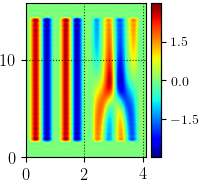
\includegraphics[width=.4\textwidth,height=.15\textheight]{MNG_001_initial}
\end{minipage}
\begin{minipage}[height=.4\textheight]{.5\textwidth}
\centering \small{\texttt{(b)}}\\
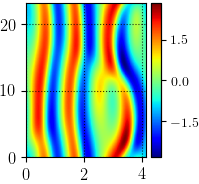
\includegraphics[width=.4\textwidth,height=.23\textheight]{MNG_001_final}
\end{minipage}
\caption{ \label{fig:block001}
(a) Initial \spt\ field for the one-by-three symbolic block given by \refeq{e-block001}
(b) \twoT\ resultant from numerically converging (a),
$[\speriod{b},\period{b}]=[4.12\cdots,23.15\cdots ]$.
}
\end{figure}




% Example that shows transformation of gap to merger
\begin{figure}
\begin{minipage}[height=.4\textheight]{.5\textwidth}
\centering \small{\texttt{(a)}}\\
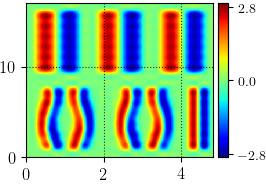
\includegraphics[width=.4\textwidth,height=.15\textheight]{MNG_000_220_initial}
\end{minipage}
\begin{minipage}[height=.4\textheight]{.5\textwidth}
\centering \small{\texttt{(b)}}\\
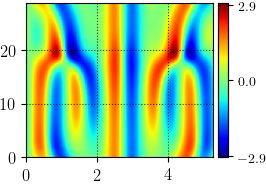
\includegraphics[width=.4\textwidth,height=.23\textheight]{MNG_000_220_final}
\end{minipage}
\caption{ \label{fig:block001}
(a) Initial \spt\ field for the one-by-three symbolic block given by \refeq{e-block001}
(b) \twoT\ resultant from numerically converging (a),
$[\speriod{b},\period{b}]=[4.12\cdots,23.15\cdots ]$.
}
\end{figure}

\begin{figure}
\begin{minipage}[height=.4\textheight]{.5\textwidth}
\centering \small{\texttt{(a)}}\\
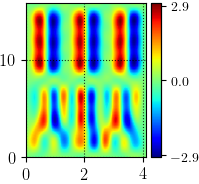
\includegraphics[width=.4\textwidth,height=.15\textheight]{MNG_000_101_initial}
\end{minipage}
\begin{minipage}[height=.4\textheight]{.5\textwidth}
\centering \small{\texttt{(b)}}\\
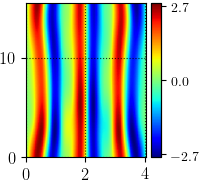
\includegraphics[width=.4\textwidth,height=.23\textheight]{MNG_000_101_final}
\end{minipage}
\caption{ \label{fig:block000_101}
(a) Initial \spt\ field for the one-by-three symbolic block given by \refeq{e-block001}
(b) \twoT\ resultant from numerically converging (a),
$[\speriod{b},\period{b}]=[4.12\cdots,23.15\cdots ]$.
}
\end{figure}

By looking at the set of converged gluings it lacks the pattern corresponding
to a gap being adjacent to a merger, spatially. %"12"
Indeed, in almost every

Here are some examples,

% Example of finding something too symmetric/shows conservation of wavenumber
%\begin{figure}
%\begin{minipage}[height=.4\textheight]{.5\textwidth}
%\centering \small{\texttt{(a)}}\\
%\includegraphics[width=.4\textwidth,height=.15\textheight]{MNG_22_11_initial}
%\end{minipage}
%\begin{minipage}[height=.4\textheight]{.5\textwidth}
%\centering \small{\texttt{(b)}}\\
%\includegraphics[width=.4\textwidth,height=.23\textheight]{MNG_22_11_final}
%\end{minipage}
%\caption{ \label{fig:block001}
%(a) Initial \spt\ field for the one-by-three symbolic block given by \refeq{e-block001}
%(b) \twoT\ resultant from numerically converging (a),
%$[\speriod{b},\period{b}]=[4.12\cdots,23.15\cdots ]$.
%}
%\end{figure}

\begin{figure}
\begin{minipage}[height=.4\textheight]{.5\textwidth}
\centering \small{\texttt{(a)}}\\
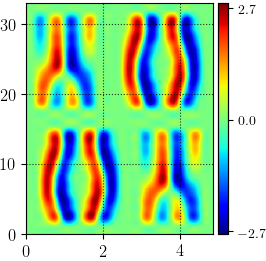
\includegraphics[width=.4\textwidth,height=.15\textheight]{MNG_12_21_initial}
\end{minipage}
\begin{minipage}[height=.4\textheight]{.5\textwidth}
\centering \small{\texttt{(b)}}\\
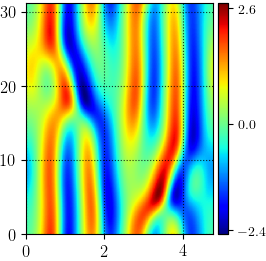
\includegraphics[width=.4\textwidth,height=.23\textheight]{MNG_12_21_final}
\end{minipage}
\caption{ \label{fig:block12_21}
(a) Initial \spt\ field for the one-by-three symbolic block given by \refeq{e-block001}
(b) \twoT\ resultant from numerically converging (a),
$[\speriod{b},\period{b}]=[4.12\cdots,23.15\cdots ]$.
}
\end{figure}

This process depends on the neighbors of the tiles as well; it seems to be primarily
influenced by spatial neighbors. For instance, in

%\begin{figure}
%\begin{minipage}[height=.4\textheight]{.5\textwidth}
%\centering \small{\texttt{(a)}}\\
%\includegraphics[width=.4\textwidth,height=.15\textheight]{MNG_002_210_initial}
%\end{minipage}
%\begin{minipage}[height=.4\textheight]{.5\textwidth}
%\centering \small{\texttt{(b)}}\\
%\includegraphics[width=.4\textwidth,height=.23\textheight]{MNG_002_210_final}
%\end{minipage}
%\caption{ \label{fig:block002_210}
%(a) Initial \spt\ field for the one-by-three symbolic block given by \refeq{e-block001}
%(b) \twoT\ resultant from numerically converging (a),
%$[\speriod{b},\period{b}]=[4.12\cdots,23.15\cdots ]$.
%}
%\end{figure}



Another common occurrence is the stretching of solutions in time where large swathes shadow
equilibria. The numerical description of this effect is that during the variational search
the time dimension being stretched, as evidenced by the large difference in time
period. This reduces the magnitude of the temporal tangents which
brings it close to equilibria In other words, stretching of the
variational ``rubber band'' kills any tangential variation. This process
is evidenced by numerical continuation of various solutions. For instance,
the merger tile has a maximum spatial domain size at which point the torus
essentially contracts into a relative equilibrium. This process is (numerically) irreversible;
reducing the domain size of the newly found relative equilibrium does not
bring the original merger tile back.


%Discussion

%Tile Families / Rubber tiles
For our purposes a collection on the order of a thousand \twots\
was collected but this was likely overkill; as seemingly indicated by the number
of fundamental tiles.

It is of course desirable to match tiles based on their boundaries as to reduce the severity of numerical
discontinuities. A more subtle reason to access the entire family is to match the
\spt\ domain size of the neighbors. Solving the optimization problem is equivalent
to enforcing the tangent space to behave according to the governing equations.
The magnitudes of the each tangent; \spt\ derivatives, are affected by the magnitude
of the temporal and spatial domain sizes.

%What is missing:
This paper mainly sets the stage and shows the feasibility for a \spt\ theory. There
is still much more work required to advance the theory.

Some of the main detractions and foreseeable criticism
% Dimensions too large



% systematic approach
Not only do we lack the symbolic
dynamics to describe infinite space-time, we also describe a smart system for enumerating all
\twots.
We currently lack a systematic approach for the enumeration of all
% symbolic dynamics
% inkling of the grammar


% no spatiotemporal theory just yet
% What advances the theory after gaining the ability to construct \twots\ from tiles?
\item[Criticisms of these methods]
Solving the linear system directly by computing the (pseudo) inverse
of the matrix
is only available for problems of dimension smaller than those that
occur in Navier-Stokes
computations. In fact, this method wouldn't be feasible in the larger
case at all and
would have to be replaced with an alternative; a common choice is to
use iterative
methods such as GMRES \rf{Saad1986}. Another aspect that has room for
improvement is
the choice of norm used in the cost function. There have been cases
where the
approximate \twot\ hardly changes (visually) even though the cost
 function is
decreasing from $10^{-4}$ to $10^{-14}$. The tolerance is strict
because we want
the best approximations possible; especially in regards to the
fundamental tiles
whose acquisition is detailed next.

Did not include considerations of local non-zero galilean velocity.

A common criticism and source of skepticism as to these methods
is the requirement
to maintain the entire \spt\ discretization in memory. While this
 is proper cause for
concern, comparisons with other studies shows a dramatic increase
in performance.
For example, in \rf{LCC06}, the tolerance was much less strict,
 the discretization
was larger, and the numerical methods required the inversion of
large matrices.

In our case, coarse \spt\ discretizations remain viable and
because the convergence is
occurring in spectral space it is not only easier to interpolate
 points (via zero padding of
the spectrum) but also produces more accurate results than with
 finite differencing.
}

\MNGpost{2020-2-21}{
\refRefs{S18, EM12, DGR97} introduce and parallelize a method known
as ``spectral deferred corrections''. \refRef{EM12} applies it
to a square $L, T = 100$
domain of the \KSe. In the applications it does not assume
periodic boundary conditions in time but
it does treat the problem spatiotemporally. The distinction
that is made is that
time integration of the discretized ODE's is not the same as
solving the underlying PDE.
\begin{quote}
\textit{In all cases, the errors reported are computed by
comparing to a temporally resolved run on the fine grid (i.e.,
 the solution of the
discretized ODE and not the solution to the underlying PDE).}
\end{quote}
They use a coarse grid to represent the solution and then
 corrections are made by solving
multi-shooting on a sequence of fine grids created via
 polynomial interpolation. Because
they interpolate, they evaluate the equations of motion
at the grid points and then use
``spectral integration'' to evaluate the integral.
\refRef{DGR97} do not use $x_{n+1}-f_n$ as their cost
function for their ``multishooting''.
For some reason their cost functions
always starts from the beginning of the fine grid and
then define the cost function to be
$x_{n+1} - (x_0 + f^{t_{n+1}}(x_0))$.
In, \rf{EM12}, the entire domain is not solved for at
the same time,
rather this process sweeps or scans through time (see figure 11).
 The parallelization
component comes in from solving the optimization problem
 on each fine grid in parallel.
The main application seems to be improving the temporal error
 introduced by time integration
schema; specifically, it provides good corrections even though
 the order of the methods
being applied in parallel are of lower order than the original method.
}

\MNGpost{2020-03-03}{
\begin{figure}
\begin{minipage}[height=.05\textheight]{\textwidth}
\centering
\includegraphics[width=1.0\textwidth,height=.2\textheight]{MNG_noise}
\end{minipage}
\caption{ \label{fig:MNGnoise}
(a) Original, converged \twot\ $[\speriod{}=21.99...,
\period{}=20.50...]$,
(b) aperiodic noise taken from standard normal distribution,
multiplied by
the $L_{\infty}$ norm of (a), (c) is the sum of (a) and (b),
(d) is the
\twot\ that (c) converges to, $[\speriod{}=22.18...,
\period{}=20.58...]$ .
}
\end{figure}

For a sense of how much noise is added, the maximum and
minimum values of
the fields in \reffig{fig:MNGnoise} are
(a) $\approx \pm 2.47$ and (c) $\approx \pm 8$. All four
fields are included
in a single figure to make it easier to have them share the
color legend.

}

\MNGpost{2020-03-03}{
\begin{figure}
\begin{minipage}[height=.05\textheight]{.5\textwidth}
\centering
\small{\texttt{(a)}} \\
\includegraphics[width=.8\textwidth,height=.2\textheight]{MNG_streak_merger_initial}
\end{minipage}
\begin{minipage}[height=.2\textheight]{.5\textwidth}
\centering
\small{\texttt{(b)}} \\
\includegraphics[width=.8\textwidth,height=.3\textheight]{MNG_streak_merger}
\end{minipage}
\caption{ \label{fig:streakmerger}
(a) Initial condition composed of three streaks and an region of zeros,
imbued on a {\spt} domain approximating the known tile's domain size.
(b) The tile that (a) converges to.
}
\end{figure}
}

\MNGpost{2020-03-03}{
Added the skeletons for the body and future work sections
of the paper.
}


\MNGpost{2020-03-05}{
Condensed version of summary. want to check the length
and wording at today's meeting.
}


\begin{figure}
\begin{minipage}[height=.05\textheight]{.5\textwidth}
\centering
\includegraphics[width=.8\textwidth,height=.2\textheight]{MNG_orbitblocktile_flow_chart}
\end{minipage}
\caption{ \label{fig:MNG_flowchart}
This flow chart represents the order that is required to make
{\spt} constructions. The flow from orbits to prime orbits to fundamental
orbits represents the process of searching for solutions and then clipping
out the fundamental tiles. Once the fundamental tiles are converged, the
fundamental tiles are well defined (the space-time on which the fundamental
orbit sits) as well as the fundamental blocks (the names that we assign
to the unique pattern found in the fundamental orbit). In order to glue,
there are three requirements, the prime configuration of blocks, the
prime tile that they are defined on, and the
approximate state that exists on the prime tile. Only after the prime
tile and prime block are in place can the fundamental orbits be
laid out on the prime tile. With this, an approximate solution that is
shadowed by a prime orbit is made. By converging this shadowed orbit
we arrive at the prime orbit it is shadowed by. Symmetry operations and
space-time periodicity then produce the entire (global) orbit.
}
\end{figure}

\MNGpost{2020-03-19}{
physicists average over everything and get some number.
Repetoire of admissible patterns, this is not the usual thing.
Full description not an average number obtained. I say
such and such patterns can exist, if this is the law that describe.

working on a problem that has been around since 1822,
a century of wrong predictions (Eulerian flows). No one
has a theory of turbulence that everyone agrees is *the* theory
of turbulence. Work on this problem at a time when the computational
methods available to me are able to describe the solutions compatible
given the equations.

Critique based on the setting, \KSe, it is not a fluid it is a one-dimensional
model but this puts me in common with many people. There is a large
population that have followed this path as a means of exploring new ideas.
Most recent nobody pays attention to it.

Approaching a problem that people understand is a problem. I am following
one line of attack which is not the historical one. Starting with the laws
and then deriving the consequences. Tackling a difficult problem which
most people use to develop techniques (KSE) (GHC N-S, C-CHristianze-Pukradtze KSe).
Not in the Kolmogorov spirit, derive some number Lots of instabilities
in space and time, not able to extend results to larger domains because
the methods we've been using are very unstable. Spatiotemporal has access
to methods that cannot be done otherwise be done. Globally they
are right and locally the
Decent solutions without insisting on a very high accuracy. Able to describe
general solution. This is exploratory and difficult problem. It is harder
than our situation because we are using $1-D$. Write it in such a way that they
do not have to stare at the equations too much as opposed to previous formulations.

More credible setting than cat map setting. Use the fundamental patterns to
describe larger and larger solutions.

The way that deciding on the fundamental patterns is done via the stability.
It is derived. Every solution has a weight that is roughly inversely proportional
to unstable directions. "There is a theory of temporal systems that says every such
solution such as the one I am finding, its importance is given by 1 over stability.
The big ones are unstable and take larger neighborhoods. When I say I have a fundamental tile,
it has a very large neighborhood. In Lorenz we say we are close to this fixed point or that fixed
point. Haven't done explicit derivation so I can only argue from analogy. The other
way is the frequency. Historically they take very narrow spatial strips and look at temporal
recurrences, more recurrences means more importances. This affects our intuition of importance.
Now we say that we are extending this idea, close recurrence in time (something that
everyone is comfortable with), and now just extending it to spacetime. Haven't
succeeded mathematically, but have succeeded in finding these solutions.

Spatiotemporal defect. Spatiotemporal chaos literature supports this name.
Number of rolls, at sometime the name changes. What it really is
in my case is the skip by $\pi / 2$ in the phase; more abstract wiggle.
wiggle, skip, swerve, curve, bend, streaks
wavy solutions at time, peaked at square root of two. Do not have wavy
structure in time.

Fixed points in time much more robust. Much more characteristic
shapes that are building up spatiotemporal solutions. GO down to
smallest possible one and call them fundamental. Use the fundamental
ones to build back up the others. Shown consistency, everything shown to the
reader is a numerically exact solution to the law (equations). On
a democratic footing. Believe solution is important because it shadows
generic {\spt} solution by being seen frequently.

Many open problems that are not covered in this first paper. Reflects
what is observed in this kind of system.
}

\MNGpost{2020-03-22}{
\textbf{Task: Library results section}
Indication of completion: when there is sufficient information
such that a reader in our field could walk away having a good idea
of what kind of solutions have been and could be found?

To this end, need to describe the types of solutions and
their importance.

Clipping and gluing {\po}s have sections dedicated to them
so this section considers everything excluding results of
those types. I am also including continuation of
in those sections because chronologically clipping precedes
finding fundamental
periodic orbits. The types of solutions remaining then amount
to the following brainstorming of examples:
\begin{itemize}
\item "homoclinic" orbit that occurs frequently in
antisymmetric subspace.
\item relative periodic
\item preperiodic
\item antisymmetric
\item eqva? reqva?
\item Solutions that would be antisymmetric
upon imposition of reflection axis. (original "po")
\item solutions seen in other papers?
\item initial conditions?
\item small
\item (relatively) large orbits
\item different members of the same group orbit.
\item "homoclinic" orbit with different symmetries
\item highly tilted rpos, nearing \reqva\, \texttt{rpo\_L24p06\_T69p30}
\item "stretched" solutions that occur near transition of unstable mode to
new frequency.
\item underresolved?
\item examples of very frequent fundamental periodic orbits shadowing
\end{itemize}

Stratifying these into categories to compile the
narrative.

\begin{itemize}
\item example initial conditions.
\item Examples of every symmetry type, size, repeats.
\item Outliers, "homoclinic", "isolated" (typically antisymmetric), rpo tilt
\item "bad" results, numerical under resolution
\item orbits which demonstrate frequent repetition of a single pattern.
\end{itemize}

Added macros for the titles of fundamental periodic orbits and
referral to the spatiotemporal domain size (lattice size? spatiotemporal area?)
as well as subdomains

}

\MNGpost{2020-03-31}{

Other {\spt} methods such as
the Newton descent method developed in \rf{lanCvit07} gave
an indication as to the typical {\spt} discretization size
required to resolve {\po}s with $L=22$ but not in the context
of \refeq{e-Fks}. Regardless of the discretization size, these
known solutions would never be solutions to \refeq{e-Fks},
due to the intrinsic error induced by numerical integration.
\refRef{EM12} summarizes this nicely by saying
 ``solving a discretized system of ODEs is
different than solving the underlying PDE''.

continuation of shift-reflect orbit as relative periodic?
maybe the shift reflect is the bisection of the "real"
fundamental periodic orbit. Look for invariants.

}


\MNGpost{2020-04-13}{

Looking forward, the main computational benefit of {\spt}
methods is that {\spt} method can be computed in parallel; therefore,
the method scales with the number of computing cores as opposed
to computing speed. The idea is to subdivide a large {\spt} domain
into small subdomains, solve the equations locally and then let
these subdomains communicate with each other.
This construction merges seamlessly with our
{\spt} theory in the context of fundamental periodic orbits.
These fundamental periodic orbits present topologically motivated
computational subdomains as opposed to arbitrary ones.
The downside, however, is that subdivision breaks the
periodic boundary conditions and hence removes the ability to
use a Fourier basis. Our intuition tells us that the best schematic
moving forward goes something like this: for dimensions of small
extent, assume periodic boundary conditions (if possible) and
use a Fourier basis. For dimensions of large extent, when it is
necessary to subdivide, use a Chebyshev polynomial basis on
the subdomains. Likewise, for non-periodic boundary conditions
we also recommend Chebyshev spectral methods. These choices
incorporate our bias against finite element methods, but as long as
the treatment is {\spt} and the inherent instability is not included,
finite element methods might have merit. This is confusing but the
concept is hard to explain and likely harder to understand.

To quell any confusion we offer the following example: it is
intuitive to imagine a $3-D$ spatial domain subdivided into
cubes (for sake of simplicity). The extension of this to $4-D$
space-time is to simply extend this subdivision so that
each subdomain is now a $4-D$ hypercubes. This is a method
to find {\po}s. Therefore the temporal dimension is always periodic.
If the temporal period is small enough that subdivision is not required,
then by following our own guidelines the computational domains
would be discretized by Chebyshev collocation points in the three
spatial dimensions but Fourier modes in the time dimension. Therefore,
in this example, the subdomains are not $4-D$ hypercubes but rather
domains with three finite dimensions (space) and one infinite dimension (time).
This is, of course, hard to visualize; at any given time the
snapshot looks like a cube, string these (periodic) snapshots together
and you get a periodic orbit. In $(2+1)$ dimensional space time the
picture that comes to mind is a toroidal solenoid with square cross section.
The usage of $4-d$ hypercubes is assuming the ``worst case'' scenario
when the computational domain is so large that each dimension \emph{has to be}
subdivided.
It may be sufficient, however, to simply increase the number of Fourier modes
(and in fact, this is what we will likely implement first).
The main reason why we include this description is to incorporate non-periodic
boundary conditions which occur in fluid dynamics calculations. Historically, these
have been handled in fluid dynamics research by the aforementioned
Chebyshev basis. This type of creative problem solving will be crucial for
solving higher dimensional equations spatiotemporally. All of this speculation
considers higher dimensional equations, but there is still much work to be
done on the theory for the \KSe.

The suspected way forward
is to use Hill's formula. Without going into too much detail, this relates
the (infinite) determinant of the Hessian of the action functional
to the characteristic polynomial of the monodromy matrix of a periodic
orbit. Simply speaking, this would allow us to relate our variational
formulation to stability, even in the absence of dynamics. % is this worth mentioning without explaining it in detail?

}

\MNGpost{2020-04-16}{
Ideas for names to replace ``symbolic dynamics''

In our previous meeting we discussed the origin of symbolic dynamics
which was to utilize discrete ``time'' to quantify chaotic dynamical systems
(period moving through a 1-D time itinerary). Obviously we want to keep the
word ``symbolic'' but we need a replacement for ``dynamics''.

The new name should be able to describe a \emph{system} with which tori
are described. In other words I believe it should account for the overarching
hypothesis that we use: infinite space-time is a collection of space-time shadowing
events. So it should be a concise way of saying ``System of symbolic representation
and shadowing?'' which does not

I think that if we can find a word that fits the phrase
``$d$\dmn\ symbolic ******'' then we will be straight.

Candidates that I've thought of to replace ``symbolic dynamics''
We likely still want to use the ``linguistics'' themed terminology
like alphabet and grammar so perhaps we should stick
\begin{itemize}
\item $d$\dmn\ symbolic syntax
\item $d$\dmn\ symbolic structuring
\item $d$\dmn\ symbolic system
\item $d$\dmn\ symbolic rendition
\item $d$\dmn\ symbolic characterization
\item $d$\dmn\ symbolic classification
\item $d$\dmn\ symbolic representation
\item $d$\dmn\ symbolic discretization
\item $d$\dmn\ symbolic presentation
\item $d$\dmn\ symbolic method
\item $d$\dmn\ symbolic fragmentation
\item $d$\dmn\ symbolic decoration
\item $d$\dmn\ symbolic marking
\item $d$\dmn\ symbolic tessellation
\item $d$\dmn\ symbolic amalgamation
\item $d$\dmn\ symbolic demarcation
\end{itemize}

We want to say that the solutions are $D+1$ tori but the notation
we decided on uses

How do we distinguish between our D+1 invariant tori and the
1-dimensional periodic orbits? We decided on using periodic orbits
and fundamental periodic orbits but I feel like this makes it seem
like we're not doing anything new.


}

\MNGpost{2020-04-17}{

%\subsubsection{numerical benefits?}
The first key difference is that the governing equation
dictates the \spt\ domain size in an unsupervised
fashion. The results here are not
The only reason why $L$ was treated as fixed is due to the
inherent instability it includes when treated as a varying quantity.
This small detail, allowing the domain size $L$ to vary,
is not as trivial as it seems.
This difficulty
is especially evident in the \KSe, whose spatial derivative terms
are of higher order than the first order time derivative, but also
there is a spatial derivative present in the nonlinear component.

}

\MNGpost{2020-04-30}{
\textbf{cut from tilebody.tex}
For example, in \rf{LanThesis} the {\spt} dimensions used to define {\po}s
was stated to be $M=32$ points in space (in their case the spatial period is fixed
at $L=22$) and either $N=512$ or $N=1024$ in time, depending on the time period.
For our methods we found that for
similar periods the spatial dimension remained the same but
the temporal dimension could be reduced to either
$N=32$ or $N-64$. This is an improvement by a factor of $16$; we emphasize
this improvement as perhaps the most common criticism
of {\spt} methods is regarding the computational memory requirements.

The most notable
is that we no longer have to grapple with exponential instabilities.
One consequence of this is that we can now find {\po}s starting only
with randomly initialized \Fcs\
defined on arbitrary {\tile}s. This specifically eliminates the time-consuming processes
of time integration and searching for close recurrences.

% tentative results from {\spt} combinations, preservation of wavenumber
Sometimes, possible improvements hint towards the grammar of the symbolic dynamics.
For instance, it seems unwise to glue the {\streak} and {\defect} temporally,
as this does not conserve the number of wavelengths; additionally,
there is a large discrepancy between the spatial periods. This implies that
a single {\streak} should not be glued in time with a {\defect}. This
configuration ({\defect} followed by two {\streak} in time) is
inconsistent in a symbolic manner.
Likewise, false positives occur when a guess for a
{\brick} converges to the ``wrong'' {\po}.
To alleviate this problem we need topological invariants which
can be used to both identify continuous families but also
the {\fpo}s they are being shadowed by.
}

\MNGpost{2020-05-03}{
\textbf{comments on determining grammar in unsupervised manner.}
As a consequence of partaking in a extensive data science / machine learning
training course I'm learning how to implement different types of neural networks.

This is likely the best manner with which to pursue automated, unsupervised identification
of {\fpo}s in {\po}s going forward. Specifically, convolutional neural networks
work very well on image recognition and there are specific techniques to ``crowd count''.
Also with the addition of details such as max pooling, the process can be robust to
translations and rotations (i.e. it has the potential to be able to
pick up different members of each {\fpo} family. It would be worth testing but
I'm guessing it will not be so easy as crowd counting techniques only count
the number of people; they do not distinguish between people. There
is also the possibility that {\fpo}s are too similar looking to be distinguished
by these methods.
}

\MNGpost{2020-05-03}{
Adding footnotes and highlights of most recent edits; the entire paper is essentially new
in the past week, however.

clipping from tilebody
In hindsight we learned that it is possible to impose shift reflection
symmetry as opposed to spatial translation symmetry, using the original
clipping as the fundamental domain. Because we know that every solution
has a reflection partner due to the symmetries of the \KSe, every
{\rpo}s exists as a pair related by reflection having equal and opposite spatial shifts.
Gluing these two solutions temporally creates and initial guess for a
shift-reflect invariant {\po}.
While not tested, it might be better to not assume relative periodicity
is that the initial guess for the spatial shift parameter is sensitive
to how the initial guess is clipped.

}

\MNGpost{2020-05-14}
{
\textbf{excerpt from "what" section.}

The nonlinear term is computed in a \emph{pseudospectral} fashion
as elementwise product in physical space as opposed to a double-convolution in Fourier space.
The definitions of each term is as follows: $\FFT$ and $\IFFT$ represent the forward and backwards
\spt\ Fourier transform operators.
Likewise, $\mathbf{\omega} = [\frac{2\pi}{\period{}},
\frac{4\pi}{\period{}},...,\frac{2\pi N}{\period{}}]$ %these are the vector of values but
and $\mathbf{k} = [\frac{2\pi}{\speriod{}}, \frac{4\pi}{\speriod{}},
...,\frac{2\pi M}{\speriod{}}]$  % technically it contains a number of repeats.
are the temporal and spatial frequencies corresponding to a set of Fourier modes.
Their multiplication with the {\spt} {\Fcs}
produces the corresponding partial derivatives through
spectral differentation \rf{Canuto88}.
Technically speaking both $\mathbf{\omega}$ and $\mathbf{k}$
actually represent a number of repeats of their frequencies; our
usage of a vectorized notation avoids indices but it should be
understood that each contains $N{\cdot}M$ values, corresponding
to the entire set of {\Fcs}.

\textbf{excerpt from gluing-what section; probably fits better in summary or results}.

We already have the two edges of this symbol plane - the $\speriod{}=22$ minimal
cell\rf{SCD07,lanCvit07} is sufficiently small that we can think of it as
a low-dimensional (``few-body'' in Gutkin and Klaus
Richter\rf{EPUR14,EDASRU14,EnUrRi15,EDUR15} condensed matter parlance)
dynamical system, the left-most column in the Gutkin and
Osipov\rf{GutOsi15} $2D$ symbolic dynamics {\spt} table (not a
1\dmn\ symbol sequence block), a column whose temporal symbolic dynamics
we will know, sooner or later. Michelson\rf{Mks86} has described the other
edge of the symbol plane, the $T=0$ line whose analogy would be ``many-body '' steady state solutions.
There are converged {\po}s which resulted from these constructions but
we have yet to determine or parse any grammar rules from said combinations.
}

\MNGpost{2020-05-14}{
Changes to tileintro: entire 'what' section reworded, symbolic dynamics
exposition and numerical explanation of Fourier mode equation pruned. (in above
blog post).

'new capabilities' in 'why' section pruned.

Initial guesses rearranged, instead of Fourier modes, then periods and discretization
it is the other way around, which is the only logical way of actually doing it (to
initialize the modes you need to know how many there are, of course).

\textbf{old gluing section}
The exact numerical choices which define the method should be treated as
preliminary ones; we believe that many improvements can (and should) be made.
The only absolute requirement with this method
that at the ``gluing boundaries'' between {\po}s or {\fpo}s there must
be an identical number of points. It is of course recommended that
the differences in periods be small but this is technically not required.
As this is the direction we are heading anyway, we shall go into
futher detail of the gluing technique
in the context of {\spt} configurations of {\fpo}s; a technique designed to
determine the admissibility of
{\brick}s of the proposed 2{\dmn} {\symbolic}.
The general case is that we have a $s_j \times s_k$ sized {\brick}.
\MNGedit{Each of these symbols represents a specific {\fpo} such that the state of
each {\brick} can be represented as the configuration of $u_j \times u_k$ {\fpo}
states. The mission is to combine these states in a numerically coherent manner.
Before we detail the choices we made, first we discuss their motivations.
There are two main sources of error resultant from gluing: discontinuities created at
the gluing boundaries and the error introduced into the tangent space by the new
approximations of $((\Delta t)_j, (\Delta x)_j)$. When combining {\fpo}s, then, it
makes sense that we make choices which attempt to reduce these factors. In the
first version of the {\fpo} gluing method, both of these are handled with zero-padding;
albeit one occurs in Fourier space and the other occurs in physical space.
The zero-padding in Fourier space is a method of interpolating points to increase
the fidelity of the velocity field state.
Each {\fpo} state is defined on a {\tile} with $(N_j, M_j)$ points and
periods $(T_j, L_j)$. The first step taken was to zero-pad the {\Fcs} of each
{\fpo}, increasing the resolution of each {\fpo}'s state. This was done
in a manner such that for each new {\tile} discretization, $(\tilde{N}_j, \tilde{M}_j)$,
the grid spacing are approximately constant between all {\fpo}s
\beq \label{e-gridspacing}
(\frac{T_j}{\tilde{N}_j}, \frac{L_j}{\tilde{M}_j}) = ((\Delta t)_j, (\Delta x)_j) \approx (\Delta t, \Delta x)\,.
\eeq
Technically these high resolution copies are no longer exact solutions, but because this is
simply a method with which to create initial guesses we deemed this as acceptable.
As previously mentioned, gluing is only well defined if the lattices being combined have the same
number of grid points along the gluing boundary.

The physical
space zero-padding is just as it sounds, a `buffer region' of zeroes is appended to each
{\fpo} state. Because it is done to each {\fpo} there will no longer be any discontinuities;
the error therefrom is instead exchanged for error in the tangent space. Dynamically, we know
that regions of zero valued velocity fields do not happen due to linear instability; the variational
formulation is able to `fill in' these regions with the correct values such that the final
state is a solution.

Therefore \refeq{e-gridspacing} will be
betrayed in one manner or another; the choice we made again utilizes padding, but this time
we zero-pad in physical space. This introduces a `buffer region' of zeros around each {\fpo}s'
original state. }
We elected for the simplest method for
approximating the new periods which is to simply add or average, depending on the gluing direction.
%alternative would be to solve the 1-d optimization problem/line search for periods. the problem with this is that increasing periods
% almost always decreases the residual.
As an example, when gluing a pair of {\po}s together in time the new temporal period for the
approximation is set to be $\period{} = \period{1} + \period{2}$ while the spatial period is
set to be $\speriod{} = \frac{\speriod{1} + \speriod{2}}{2}$ (if the gluing was in space, the average and
summation operations would be permuted).
In this case the number of spatial grid \emph{points} %describe additional fpo gluing actions.
and temporal grid \emph{spacing} are made to be the same.
These choices become less obvious when gluing is extended to
arbitrary {\spt} combinations. The difficulty arises from maintaining
as uniform of a grid spacing as possible while also
satisfying the requirement for the equal number of points along
each boundary. The current implementation combines the gluing
methods for space and time by building up {\spt} combinations via
spatial or temporal strips. This worked sufficiently well such that
``full'' gluing process defined by gluing all constituents in a single step was left for future work.

}

\MNGpost{2020-05-15}{
\textbf{intro, why, excerpts}
The variational formulation does not completely remove
all challenges, however, such as finding
{\po}s on large {\spt} domains. However
for our purposes we have no need to confront this challenge directly.
The current goal is to find only the most important {\fpo}s; believed to
exist only on small {\spt} domains.

\textbf{intro, what, excerpts}
 There is no
guarantee that the final periods will be near the original values, but the idea
is that these initial guesses start closer, and hence converge, to {\po}s of similar size.

That is to say, the corresponding
region of discretized configuration space and the overlying state are extracted; providing
an initial guess for an {\fpo} (or {\po}, depending upon what is clipped) which is
passed to our optimization methods.

In regards to the \KSe, the clipping is currently a single step procedure; however,
we shall demonstrate an iterative usage as other systems may not have this luxury.
The process of finding {\fpo}s via clipping is the process of distilling large
{\po}s into small {\po}s. This smoothed
initial guess is then used to search for a {\po}. Arbitrary {\fpo} combinations are
not guaranteed to represent {\po}s; this property is encapsulated by the {\symbolic}
that we are developing. In other words, gluing constitutes an empirical method
used to probe and uncover a 2\dmn\ {\spt} {\symbolic}. Specifically the gluing process
as it has just been described is the method that converts {\brick}s into
initial guesses for the corresponding {\po}s.

As a reminder, our collection of {\po}s need not range over all sizes;
which we believe manifest as {\po}s with small periods. Therefore,
the search for {\po}s was limited to what we consider as intermediate domain sizes.
Periods were chosen from the ranges
$\period{}\in [20, 180]$ and $\speriod{} \in [22, 88]$.

but were typically chosen to be powers of two; in order
to leverage fast Fourier transforms. %reference
Typically, we used a rule of thumb which set the number of points in the
spatial dimension as $M = 2^{\lfloor\log_2(\speriod{})\rfloor + 1}$
and the number of points in the temporal dimension as
$
N = 2^{\lfloor\log_2(\period{})\rfloor}\,.
$

\textbf{intro, how, excerpts}
As previously mentioned, we do not use
approximate recurrences nor time integration
to generate initial guesses.
Instead, initial guesses can be generated by initializing arbitrarily
sized domains with random noise.
More specifically, random values are drawn from the standard normal distribution
and assigned as the values of the corresponding Fourier modes.
These modes may then rescaled in a manner that befits a
doubly periodic solution of the {\KSe},
manipulating the Fourier spectrum to match the relevant scales of the \KSe.
In our experience, however, the initial guesses which are `worse' with respect
to the cost function actually converge more often; or, equivalently by our standards,
they seem to get trapped by local minima less often.
It is therefore hard to provide a recommendation for a single or `best'
manner with which to provide initial guesses. The
numerical methods we employ do not seem to be interested in our desire
to produce a physically motivated construction method
drawn from our experience and intuition.

The termination of the descent is determined by either error threshold
or step limit; though there are arguably better termination conditions such as the Wolfe or
Goldstein conditions.


Euler's
method is used because it is the simplest and fastest integration scheme.
The integration need only be as accurate as necessary to decrease the cost function;
we only care as to whether we are approaching a {\po} or not.


The first is to solve \refeq{e-newton} in a least-squares manner \rf{Dennis96},
the second is to include constraints which make the system square, the third is to solve
the system of \textit{normal equations} which result from multiplication of both sides of
\refeq{e-newton} by $\nabla\mathbf{F}^{\top}$.
We are not focused on finding unique or specific solutions (a specific member of a group
orbit, uniquely determined by a square, invertible linear system).
In fact, it is to our advantage to do exactly the opposite: increase the frequency of convergence
by allowing for any member of a group orbit.
The price of this is the acceptance that calculations may be redundant; however,
the number of {\po}s being infinite this seemed unlikely to be exceptionally
dangerous. Hereafter it shall always
be implied that any discussion pertaining to solving \refeq{e-newton} shall be in a least-squares
sense.

 This is
done in an inexact manner instead of finding the optimal step length, as
would be the case in a line search. Specifically, we simply halve the step length
until one of the criteria is met.

For the numerical methods, a handful of parameters are required such as the step limit
and tolerance. Our typical choices, noting that they are likely suboptimal, are as follows:
the tolerance of the cost function for the gradient descent was $J = 10^{-4}$
and the step limit was set to a multiple of the dimension, either $16NM$ or $32NM$.
This means that if either \refeq{e-cost} $J < 10^{-4}$ or the step limit
is reached, then the descent method terminates, and the guess is passed to the
least-squares implementation.
The ``heavy lifting'' was delegated to the least-squares method
with backtracking. The threshold for termination was originally set to double
floating point precision but over time this was relaxed to incorporate the {\em cdof}, i.e.
the current tolerance is on the order of $(NM)*10^{-15}$; and the step limit, $500$.
For those familiar with Newton methods, this number of steps appears like overkill at first, but the
allowance of backtracking negatively impacts the rate of convergence.

The clipping process by definition returns initial guesses which
are not doubly-periodic. To mitigate the error introduced by this we always
increased the resolution prior to clipping and decrease it afterwards by means
of zero-padding and Galerkin truncation of the {\Fcs}, respectively.

This was especially true in the cases where the suspected
{\fpo}s were {\rpo}s.


Clipping can be described quantitatively as follows.
Let the dimensions of the original {\po} be $x \in [0, \speriod{0}]$,
$t \in [0, \period{0}]$ defined on a {\spt} lattice with $N\times M$ sites.
To create an initial guess via clipping, choose a rectangular subregion of the original {\po}'s discretization,
$n\leq N, m\leq M$. The periods are then given by the appropriate fractions of the original,
$\period{c} = \frac{\period{}n}{N}$ and $\speriod{c} = \frac{\speriod{}m}{M}$.
Because translation is free, the domain is relocated to the origin, such that the result
is an initial guess $u_c(x,t)$ with $0 \leq t \leq \period{c}$, $0 \leq x \leq \speriod{c}$,
where $u_c(x,t)$

he clipping process creates an initial guess with periods , where $n$ and $m$ represent the number of points in time
and space which define the clipping's discretization. . Because translation
is a free action, we say that the clipping is now


The main challenge of gluing is reconciling the differing discretizations and periods
of the {\fpo}s. Discretization by itself is a non-issue; one simply pads or truncates the Fourier
spectrum such that along every shared boundary, each {\fpo} has the same number of points.
The {\fpo}s have different periods, however, so if they have an equal number of points that
implies that they have an unequal grid spacing ($\Delta t$ or $\Delta x$). This discrepancy
affects the magnitudes of tangents and hence the quality of the gluing. In purely
practical terms, the gluing of large arrangements of {\fpo}s in a single step is more
complex simply due to the number of boundaries. To deal with this complexity, a methodology
is required; our prototype is an extension of pair-wise gluing, which shall be described now.

For notational purposes, let us call refer to
the pair of orbits as orbit A and orbit B.
As a preprocessing step these orbits are rediscretized
so that they all have equal grid spacings.
This seems to contradict our previous
statements, but the initial uniformity allows for a tidier description.
For sake of argument we'll be using space as the `gluing direction'; the solutions
are concatenated spatially.
To retrieve the temporal gluing method, simply permute all mentions
of space and time.  Let orbit A be
defined with periods $[\period{a}, \speriod{a}]$, on a discretization with $[N_a, M_a]$
points in time and space, respectively. Likewise for orbit B. When gluing in space, we
set the temporal period of the gluing to be the average of the original periods,
$\period{ab}=\frac{\period{a}+\period{b}}{2}$. This, in combination with the
fact that the number of points in the \emph{time} dimension must be the same,
leads us to rediscretize each orbit such that the new number of points
in time is also the average of the originals
$N_{ab} = \frac{N_a + N_b}{2}$. For space, no rediscretization is required,
because the preprocessing step made the spatial grid spacings equal. Similarly, the
new spatial period is simply set to be the sum of the originals $\speriod{ab}
= \speriod{a} + \speriod{b}$. This choice may seem poor at first; the spatial period of
the {\po} being shadowed by two constituents would be guaranteed to be larger than this sum
(imagine a figure eight being shadowed by two circles). More precisely,
$\speriod{ab} > \speriod{a}+\speriod{b}$ would be satisfied
However, because we allow \emph{both} time and space periods to change, it is possible
to find a member of the shadowed orbit's family which does not satisfy this inequality.
Now that we have the periods and discretization of the gluing, we can give it a precise
definition. This particular gluing results in a field defined on a {\tile} of dimensions
$[\period{ab}, \speriod{ab}]$ and $N_{ab}{\times}M_{ab}$ points. The field is now
piecewise defined such that
\beq u_{ab}(x,t) =
    \begin{cases}
      u_{a}(x,t) & 0 \leq x \leq \speriod{a}\,,\; 0 \leq t \leq \period{ab}  \\
      u_{b}(x,t) & \speriod{a} \leq x \leq \speriod{b}\,,\; 0 \leq t \leq \period{ab} \\
    \end{cases}
\eeq
with boundary conditions $u_{ab}(0,0) = u_{ab}(\speriod{ab},0) = u_{ab}(0,\period{ab}) = u_{ab}(\speriod{ab},\period{ab})$

This concludes the pairwise gluing method, in summary, in the gluing direction the number of
points and periods are additive and in the transverse dimension these quantities are averaged.



There was no clear manner with how to proceed with gluing large arrangements of {\fpo}s;
our prototype is an extension of the pairwise gluing method.
Let us represent the arrangement of {\fpo}s as an array, where the rows correspond to time and
the columns, space. For space-time gluing,
we elect to first glue the {\fpo}s into spatial strips, and then glue them
in time. For example, let us have a $3x3$ array of {\fpo}s.
First, we glue each row together (spatial gluing), creating a $3x1$ array; the time period
of each row come from averaging and the spatial period comes from summation. Then we glue these strips
in time; such that now the time periods ares summed and the spatial periods, added.
This produces the final gluing result: the final periods end up being the total sum, divided
by the number of rows and columns in the array of {\fpo}s; in this example, the resultant periods are
$\period{} = \frac{1}{3} \sum \period{ij}$ and $\speriod{} = \frac{1}{3} \sum \speriod{ij}$
We propose some alternative methods for this in \refsect{sect:summary}
but currently, they are not fully developed.

The main challenge of gluing is reconciling the differing discretizations and periods
of the {\fpo}s. Discretization by itself is a non-issue; one simply pads or truncates the Fourier
spectrum such that along every shared boundary, each {\fpo} has the same number of points.
The {\fpo}s have different periods, however, so if they have an equal number of points that
implies that they have an unequal grid spacing ($\Delta t$ or $\Delta x$). This discrepancy
affects the magnitudes of tangents and hence the quality of the gluing. In purely
practical terms, the gluing of large arrangements of {\fpo}s in a single step is more
complex simply due to the number of boundaries. To deal with this complexity, a methodology
is required; our prototype is an extension of pair-wise gluing, which shall be described now.


\textbf{summary excerpts}
The difficulties are described here in the context of
periodic orbit theory specifically cycle expansions. Cycle
expansions are quantitative descriptions of
chaotic attractors via summation over
an infinite collection of prime orbits. This collection has a well defined
hierarchy of importance as determined by {\po}'s temporal periods and stability. This
ranking is critical as it dictates how to truncate the infinite sum resulting
from cycle expansion.
In our case, however, we do not know what constitutes ``primeness'' with respect to
continuous families. In addition, we currently do not have a manner with
which to compute {\spt} topological invariants. In other words, we do not know
how to rank and sum over {\po}s in our description.
Our intuition tells us that the analogous quantity to temporal periods should
be the {\spt} area but this has not yet been confirmed explored.
}

\MNGpost{2020-08-13}{
Finally finished with data science / machine learning / deep learning / neural network certification program.

Roadmap for the next three months:

\begin{enumerate}
\item Finish Thesis
\item Finish Thesis presentation
\item Finish orbithunter (my python package) documentation, included in thesis
\item Discuss randomly connected RNN with Schatz, Grigoriev group.
\item (external to Physics) find a job, work on CNN symbolic dynamics
\item Future projects TBD.
\end{enumerate}

}

\MNGpost{2020-10-08}{
I've looked and asked around but I cannot find an answer to a very simple
question; I've attached it as an image.

% \includegraphics[width=.9\textwidth]{MNG_projection}

For context: the projections I
will actually be describing are projections onto symmetry invariant
subspaces, the image is just a toy example of what I mean. I understand
that the functions (in the image) are formally equivalent to one another
but I am trying to explain that they are different numerically because
the latter reduces the number of computational degrees of freedom. The
example uses functions, but technically I am trying to explain the
distinction in the context of matrix representations.

Is there a word for this distinction, or does one have to explicitly
include it in the definition?
}

    \PCpost{2020-10-09}{
mhm... In birdtracks.eu
\HREF{http://birdtracks.eu/version9.0/GroupTheory.pdf\#section.3.6}
{eq.~(3.60)}
I think of each sub-block as a matrix of lower dimension.
I would never write $\phi({\bf v})=\transp{[x,y,0]}$, only
$\phi({\bf v}^{(\alpha)})=\transp{[x,y]}$, in the $\alpha$ irrep.
    }

    \PCpost{2020-10-10}{
I'll talk in \HREF{http://csp2020.ac.ru/program.html}
{Moscow Monday morning} about our spatiotemporal ideas,
so I'm having a look at recent papers on variational methods:

Kerswell
\HREF{https://www.damtp.cam.ac.uk/user/rrk26/Udine_LT56_RRK.pdf}
{Exact Coherent States: Variational Methods} lectures look good.

Daniel Lecoanet \etal\ \HREF{https://doi.org/10.1103/PhysRevResearch.2.023068}
{Daedalus} deserves a look.

Brunton \etal \HREF{https://doi.org/10.1146/annurev-fluid-010719-060214}
{Machine Learning for Fluid Mechanics} - have not checked it yet.
    }

\item[2020-10-22 Erik Aurell].

Title: Spatiotemporal tiling of the Kuramoto-Sivashinsky equation
\\
Speaker: Matthew Gudorf (Georgia Tech)
\\
Time \& place: Thursday October 22 at 13.00 on zoom

Abstract:
Motivated by space-time translational invariance, `spatiotemporally
chaotic' or `turbulent' flows are recast as a (D+1)-dimensional
spatiotemporal theory which treats space and time equally. In this
formulation time evolution is replaced by a repertoire of spatiotemporal
patterns taking the form of (D+1) dimensional invariant tori. Infinite
space-time is then explained by the shadowing of these tori. This is
formalized by the development of a (D+1)-dimensional symbolic dynamics
whose alphabet is comprised of space-time tori of minimal size.
Enumerating these spatiotemporal building blocks enables the construction
of all admissible spatiotemporal patterns. These ideas are investigated
in the context of the Kuramoto-Sivashinsky equation using new, open
source spatiotemporal computational computing package 'orbithunter'.
These codes are designed to offer easy access to new spatiotemporal
techniques, persistent homology, convolutional neural networks and more.

The talk was not recorded.
For seminars in the CS \& BP series, see
\HREF{http://agenda.albanova.se/categoryDisplay.py?categId=253} {here}.

\MNGpost{2020-10-22}{

Karoshi which can be translated literally as ``overwork death" is a Japanese term relating to occupational sudden mortality. The most common medical causes of karoshi deaths are heart attacks or strokes due to stress and a starvation diet. Mental stress from the workplace can also cause karoshi through workers taking their own lives. People who commit suicide due to overwork are called karojisatsu. The phenomenon of death by overwork is also widespread in other parts of Asia.

I have worked out enough that I believe in my cardio but random palpitations and arrhythmia have me shook; probably psychosomatic.
One last sprint to the finish....
    }

\PCpost{2020-10-25}{
No karoshi, please, we already have fascists and COVID-19 to stress us out.

\HREF{https://www.youtube.com/watch?v=wugWGhItaQA}
{Just play it cool, boy, Real cool!}.
    }

\begin{figure}
\begin{minipage}{.45\textwidth}
\centering
\includegraphics[width=1\textwidth, height=0.28\textheight]{EquilibriumOrbitKS_L3974779240p595_parametric_plot_u_ux}
\end{minipage}
~~~
\begin{minipage}{.45\textwidth}
\centering
\includegraphics[width=1\textwidth, height=0.3\textheight]{EquilibriumOrbitKS_L3974779240p595_modes}
\end{minipage}
\caption{\label{fig:MNG_Linfty_u_vs_ux}
(left) Parametric plot of $u_x(x)$ vs. $u(x)$ for $L\approx 3974779240$ \eqv.
As the stable ``cells" of
Frisch, She and Thual\rf{FSTks86}, this \eqv\ belongs to the asymmetric subspace,
but as it has a number of winds it is (presumably) unstable.
(right)
Fourier coefficients $-i\,c_{0k}$.
See the thesis\rf{GudorfThesis} for definitions, spatially antisymmetric
zeroth time $k$th spatial modes.
}
\end{figure}

\begin{figure}
\begin{minipage}{.45\textwidth}
\centering
\includegraphics[width=1\textwidth, height=0.3\textheight]{EquilibriumOrbitKS_L3974779240p595_uux_modes}
\end{minipage}
~~~
\begin{minipage}{.45\textwidth}
\centering
\includegraphics[width=1\textwidth, height=0.3\textheight]{EquilibriumOrbitKS_L3974779240p595_uxx_modes}
\end{minipage}
\caption{\label{fig:MNG_Linfty_uux_modes}
(left) Modes of $uu_{x}$ for $L\approx 3974779240$ \eqv.
They are approximately the negative of
(right) $u_{xx}$  modes, in agreement with the wrong sign diffusion term
``Burgers'' eq.~\refeq{WrongBurgers} for an \eqv; the difference is the
vanishingly small  $u_{xxxx}$ that can be neglected for such long
wavelength solutions.
} % \reffig{fig:MNG_Linfty_uxx_modes}.}
\end{figure}

\MNGpost{2020-10-22}{
I found some big boys...like really big.... like a $L = 4 \cdot 10^{9}$
big \eqv. The modes with all of the energy are multiples of $32n$ for a
reason unknown to me other than simply saying 'aliasing'. I obviously do
not have enough modes to resolve all scales but hey its kinda cool.

I can't tell if this is an interesting result, or if it's
already known solutions from Michelson\rf{Mks86} or
similar? The fourth derivative gets killed, so that the
equations, for practical purposes, reduce to
\beq
u_t + u\,u_x = -u_{xx}
\,.
\ee{WrongBurgers}
I double checked it and I stand by the values,
however I don't know if its worth anything. Some of the figures do not
fit on the page so look for them in \emph{/figs/}.
    }

    \PCpost{2020-10-25}{
I suspect your $32n$ are the stable ``cells" of
Frisch, She and Thual\rf{FSTks86} {\em Viscoelastic
behaviour of cellular solutions to the Kuramoto-Sivashinsky model}
(1986). Have to convert the units as in ChaosBook
\HREF{http://chaosbook.org/chapters/ChaosBook.pdf\#section.30.1}
{sect.~30.1.1} {\em Symmetries of Kuramoto-Sivashinsky equation}
to compare.

``The fourth derivative getting killed'' would make them into
solutions of the wrong sign Burger's equation \refeq{WrongBurgers}.

I looked into  \emph{/figs/}, but there is nothing there other than
\reffig{fig:MNG_Linfty_u_vs_ux} and \ref{fig:MNG_Linfty_uux_modes}.
{\em EquilibriumOrbitKS\_L3974779240p595\_field\_fdomain.png} color plot
is not informative,
for \eqva\ one plots $u(x)$ on $[0,\speriod{}/2]$.
    }

    \PCpost{2020-10-25}{
Aren't you plotting twice as many wave-numbers in
\reffig{fig:MNG_Linfty_u_vs_ux}\,(right) (right) as needed for an
antisymmetric subspace solution? But then I do not understand the
$k$-axis in \reffig{fig:MNG_Linfty_uux_modes}, these do not mach up -
should you get the same non-vanishing modes in all three figures?
    }

    \PCpost{2020-10-25}{
The single, universal, correct spatial mode-indexing
convention\rf{DCTSCD14} for {\large all} \KS\ documents that we produce:

The horizontal, eigenmode / wavenumber axis should always be
$j/\tildeL=2\pi{j/L}$, and, due to the $\On{2}$ having 2-dimensional
irreducible representations
(sines \& cosines, rather than $\exp(i2\pi{j}/\speriod{})$'s)
one should always group Floquet exponents (and, I believe, Fourier modes
as well) into $j,j+1$ pairs, plot them as a single, two-valued $j$.

I think you also want to use logarithmic scale on the $y$-axis, as
everything is expected to fall off exponentially or faster for modes
beyond the entangled, ``physical'', inertial-manifold modes. To trust
your calculation, you always want to capture the beginning of the
transient, ``unphysical'' modes in your spectrum.

What one chooses to pair for low $j$ might be ambiguous, as the nonlinear
interactions mix up the $\On{2}$ 2-dimensional linearly irreducible
representations.

This way wave-number plots for any \speriod{} have the same
$x$ axis.

Should you know of any reason that we should not be joined in holy
notational convention, speak now or forever hold your peace.

If you agree, follow our convention in ALL plots, it's our misfortune
that none living has as much experience with \KS\ as we do.
    }


\MNGpost{2021-04-12}{
Getting really close to being able to find very {\Large very large}
periodic orbits. In \reffig{fig:cfwinit}\,(a) the resolution is due to
computational degrees of freedom; small amount of interpolation but too
much would distort the field and make it look non-physical. For
\reffig{fig:cfw}\,(b) the residual is $\mathcal{O}(10^{-2})$; for a solution
this large I find this to be quite the achievement. Requires lots of
supervision however, to create an initial guess.

\begin{figure}
\begin{minipage}[height=\textheight]{\textwidth}
\centering \small{\texttt{(a)}}\\
\includegraphics[width=\textwidth,height=.5\textheight]{county_fair_winner_initial}
\end{minipage}
\caption{ \label{fig:cfwinit}
(a) Initial guess for orbit hunting.
Periods $(\speriod{},\period{})\approx(500,488)$.
}
\end{figure}

\begin{figure}
\begin{minipage}[height=\textheight]{\textwidth}
\centering \small{\texttt{(b)}}\\
\includegraphics[width=\textwidth, height=.7\textheight]{county_fair_winner}
\end{minipage}
\caption{ \label{fig:cfw}
(b) Final result after about 6 hours (on my laptop) of application of
conjugate gradient method. Dimensions
$(\speriod{},\period{})\approx(555,783)$. Discretization included 512 in
space, 128 points in time, hence low resolution figure.
}
\end{figure}

Getting very close to finding arbitrarily large periodic orbits for \KSe, however, when trying
to develop a guide by implementing the Lorenz equations, the code fails quite miserably, when
$\sigma, b, \rho$ are fixed. In other words, discrete dimensions provide yet another challenge.
Unsure if unpalatable but my gut is telling me the quasi 2-d nature of the Lorenz attractor is causing
this, meaning that for "extra flexibility", unconstrained parameters are needed, as I do not believe
that the attractor would remain in the same plane, just my two cents.
}

\PCpost{2021-04-16}{
Interesting.

You started with $u$ guess in range $u\in[-3.3,3.3]$ and - even though
the resulting solution is stretched out by 50\% in time, the $u$ range is
barely bigger, $u\in[-3.8,3.8]$. So somehow if you start with atypical
guess pattern (no random walk in the local mean $u$), you end with
atypical solution.

Contrast with $u\in[-5,5]$ of \reffig{fig:MNGlarge_adjointdescent} (and
many large spacetime figures currently commented out, but fine
otherwise). As I explain above (see {\bf 2019-05-13 Predrag} post), we
expect the range of the color bar in such figures to grow proportionally
to $\sqrt{\speriod{}}$.
}



\end{description}
%%%%%%%%%%%%%%%%%%%%%%%%%%%%%%%%%%%%%%%%%%%%%%%%%%%%%%%%%%%%%%%%%%%%%%%
\printbibliography[heading=subbibintoc,title={References}]
